
\documentclass[a4paper, 12pt, oneside, BCOR1cm,toc=chapterentrywithdots,hidelinks]{scrbook}

\usepackage[a4paper]{geometry}
\usepackage{textcomp}
\usepackage{longtable}
%\usepackage{tabu}

\usepackage[ngerman, english]{babel}
\usepackage[utf8]{inputenc}
\usepackage{graphicx} 
\usepackage{url}           	 
\usepackage{hyperref} 	
\usepackage{listings, color}	% for source code
\usepackage{scrlayer-scrpage}	% header and footer line
\usepackage[nohyperlinks]{acronym}
\usepackage[ruled,vlined,algochapter]{algorithm2e}
\usepackage{tocbibind}
\usepackage{blindtext}
\usepackage{titling}


\usepackage{chngcntr}
\counterwithout{figure}{chapter}
\counterwithout{table}{chapter}
\counterwithout{algocf}{chapter} 
%\counterwithout{lstlisting}{chapter}
\AtBeginDocument{% the counter is defined later
  \counterwithout{lstlisting}{chapter}%
}
\renewcommand\lstlistingname{Code Fragment}

%for adding comments
\usepackage{verbatim}

% Placeholder box for figures that are not yet produced.
% Usage: \figplaceholder{description of the planned figure}{caption}{fig:label}
\newcommand{\figplaceholder}[3]{%
  \begin{figure}[ht]
    \centering
    \fbox{\parbox[c][6cm][c]{0.85\textwidth}{\centering
      \textbf{[Figure placeholder]}\\[0.6em]\small #1}}
    \caption{#2}
    \label{#3}
  \end{figure}}

% for tables
\usepackage{multirow}
\usepackage[table]{xcolor}
\usepackage{xcolor}

% for the architecture figure (figures/spillable_slice_store.tex) — after xcolor to avoid option clash
\usepackage{tikz}
\usetikzlibrary{positioning,arrows.meta,shapes.geometric,fit,backgrounds,calc}

% header and footer line - no header & footer line on pages where a new chapter starts
\pagestyle{scrheadings}
% TU Berlin logo at header
\chead{
\includegraphics[width=1.2cm]{./img/TU-Berlin-Logo.pdf}
}



\newcommand{\tTitle}{Out-of-Core Stream Processing in NebulaStream}
\newcommand{\tSubtitle}{A RocksDB-Based State Backend for Memory-Constrained Edge Devices}
\newcommand{\tAuthor}{Benjamin Sainsanaa Steinb\"uchel}
\newcommand{\tMatknr}{396953}
\newcommand{\tEmail}{b.steinbuechel@campus.tu-berlin.de}
\newcommand{\tDegreeProgramme}{Computer Engineering}
\newcommand{\tDegreeType}{Bachelor's}
\newcommand{\tPrimaryReviewer}{Prof.\ Dr.\ Volker Markl}
\newcommand{\tSecondaryReviewers}{Prof.\ Dr.\ Matthias B\"ohm}
\newcommand{\tAdvisors}{Leonhard Rose}





\begin{document}

\frontmatter

%Titlepage
\thispagestyle{empty}
\begin{center}

\begin{figure}[t]
    \centering
    
\includegraphics[width=3cm]{./img/TU-Berlin-Logo.pdf}%
%    \qquad
%    \includegraphics[width=3.3cm]{dima_logo.png}%
\end{figure}

%\vspace*{0.2cm}
{\LARGE \textbf{Technische Universit\"at Berlin}}

\vspace{0.5cm}

{\large Chair of Database Systems and Information Management\\[1.6mm]}
%{\large Fachgebiet Datenbanksysteme und Informationsmanagement\\[5mm]}

%Fakult\"at IV\\
%Einsteinufer 17\\
%10587 Berlin\\
%https://www.dima.tu-berlin.de\\

\vspace{1.5cm}

{\Large Bachelor's/Master's Thesis}\\

\vspace{1.0cm}
{\LARGE \textbf{\tTitle}}\\
\vspace{0.5cm}
{\large \textbf{\tSubtitle}}\\
%\vspace*{0.3cm}
%{\LARGE \textbf{second Line}}\\
\vspace{1.0cm}
%{\LARGE Firstname Lastname(s)}
%\vspace*{0.5cm}
\tAuthor, \url{\tEmail} \\
Degree: \tDegreeProgramme\\
Matriculation Number: \tMatknr\\

\vspace*{2.0cm}
\textbf{Reviewers}\\
\tPrimaryReviewer \\
\tSecondaryReviewers \\
\vspace*{0.5cm}
\textbf{Advisor(s)}\\
\tAdvisors \\
\vspace{0.5 cm}

\textbf{Submission Date}\\
\today\\ % 	date of submission
\end{center}


\thispagestyle{empty}
\cleardoublepage
    
%Self-assertion
%\newpage

\section*{Selbstständigkeitserklärung}

\noindent
Hiermit versichere ich, dass ich die vorliegende Arbeit ohne Hilfe Dritter und ausschließlich unter Verwendung der aufgeführten Quellen und Hilfsmittel angefertigt habe.
Alle Stellen die den benutzten Quellen und
Hilfsmitteln wörtlich oder inhaltlich entnommen sind, habe ich als solche kenntlich gemacht.
Sofern KI-Tools verwendet wurden, habe ich Produktnamen, Hersteller, die jeweils verwendete Softwareversion und die Art der Nutzung (z.B. sprachliche Überprüfung und Verbesserung der Texte, systematische Recherche) benannt.
Ich verantworte die Auswahl, die Übernahme und sämtliche Ergebnisse des von mir verwendeten KI-generierten Outputs vollumfänglich selbst.


Die Satzung zur Sicherung guter wissenschaftlicher Praxis an der TU Berlin vom 15. Februar 2023 habe ich zur Kenntnis genommen.

Ich erkläre weiterhin, dass ich die Arbeit in gleicher oder ähnlicher Form noch keiner anderen Prüfungsbehörde vorgelegt habe.
\vspace{2cm}

\noindent
Berlin, \today

\vspace{3cm}

\begin{flushright}
    \hspace*{6cm}%
\dotfill\\

\textit{\tAuthor}

\end{flushright} % choose either this...
\newpage


\section*{Declaration of Authorship}

I hereby declare that the thesis submitted is my own, unaided work, completed without any external help.
Only the sources and resources listed were used.
All passages taken from the sources and aids used, either unchanged or paraphrased, have been marked as such.
Where generative AI tools were used, I have indicated the product name, manufacturer, the software version used, as well as the respective purpose (e.g. checking and improving language in the texts, systematic research).
I am fully responsible for the selection, adoption, and all results of the AI-generated output I use.

I have taken note of the Principles for Ensuring Good Research Practice at TU Berlin dated 15 February 2023.

I further declare that I have not submitted the thesis in the same or similar form to any other examination authority.

\vspace{2cm}

\noindent
Berlin, \today

\vspace{3cm}


\begin{flushright}
    \hspace*{6cm}%
\dotfill\\

\textit{\tAuthor}

\end{flushright}

 % ...or this
\newpage
\section*{Documentation of Tool Usage}
In accordance with the requirements for good scientific practice, below I have documented my use of (AI) tools in the process of writing this thesis.

% Let the long archive URL wrap at path separators instead of running off the page.
% Without this, \url treats it as one 706pt box against a 418pt textwidth.
\expandafter\def\expandafter\UrlBreaks\expandafter{\UrlBreaks\do\/\do\-\do\.\do\_}

\noindent The \emph{Link to Prompts} column resolves to the public archive

\begin{center}
\small\url{https://github.com/Oblision/Bachelor-Thesis-RocksDB-IoT/tree/main/nebulastream-Out-of-Core-Stream-Processing/docs/ai-usage}
\end{center}

\noindent Phases 1--3 preceded this thesis as part of the accepted proposal; their folders hold browser captures of the conversations. Phases 4--8 hold one Markdown file per archived conversation, with the verbatim prompt, the full transcript, and the model recorded for that conversation.
Where several tools were used within one phase, that phase has one line per tool.
The manufacturers of the tools named below are OpenAI (ChatGPT), Anthropic (Claude), and Grammarly, Inc.\ (Grammarly); the parenthesised name on a Claude line is the application it was accessed through.
\vspace{0.5cm}

% ---------------------------------------------------------------------------
% TODO (Benjamin) — Levels of Use are PROPOSALS; confirm each before signing.
%   Ph.1  2 — settled with the author 2026-07-16. The tool was used to understand
%         the offered topics and the terminology (alignment, inference, concurrency,
%         hash vs sort, aggregation types) before committing time to one: the
%         level-2 example "requested explanations of individual terms in the
%         assignment". Not 1: the author states he took substantial insight from it.
%         Not 3: level 3's marker is "iteratively adding the model's output", and
%         none was added — LMDB, spill policy, the 48-run matrix and the >=20% tail
%         target all return 0 hits in chapters/. Residual argument for 3: level 3
%         also lists "suggested possible topic outlines", and on 2025-10-14 the model
%         volunteered scope options A/B/C unprompted; the delivered scope resembles
%         its option A, though scope was settled with the advisor in the meeting.
%         Provenance of the key decision: the author was leaning LMDB; the advisor
%         steered to RocksDB and the author adhered. LMDB: 0 hits; RocksDB: 7 files.
%   Ph.2  3: on 2025-11-02 the model volunteered thesis-ready prose. Not adopted —
%         SliceStoreManager, soft/hard watermark, buffered sequential I/O,
%         TupleBuffer, "transparency", "synchronous overhead": 0 hits in chapters/.
%   Ph.3  4 — settled with the author 2026-07-16. The 2026-02-04 conversation began as
%         "is YSB suitable" but became an evaluation-design session: the model proposed
%         characterising workloads by stress properties over a named benchmark, via a
%         parameterised synthetic generator (key_space_size, window_size, event_rate,
%         skew_factor) under a fixed container RAM limit with swap disabled. The author
%         confirms the evaluation design came substantially from it. Corroborating greps:
%         synthetic(1), zipf(1), skew(1), cardinality(2), swap(2), cgroup(3), NexMark(2),
%         plus the repo folder evaluation-10k-synthetic. NOT adopted: burst(0),
%         hot/cold(0), "PSSW"(0), YSB itself. Filed under 03 at the author's direction;
%         the design it shaped is implemented under phase 5, which already declares 4.
%   Ph.4-8 corrected against the archive frontmatter 2026-07-16.
%
% STILL OPEN:
%   - CODEX: not a tool that was used. The 2025-11-02 prompt says "diese comments
%     von codex generiert", but the author confirms this was a misnomer for ChatGPT;
%     OpenAI Codex was not used. Noted in the 02 entry so the archive and the
%     capture do not appear to contradict each other.
%   - Two claude.ai chats unplaced (share links in proposal-phase.md).
%   - Sidebar shows unreviewed chats ("Thesis Question Recomme...", "Anwendung vs
%     Thread", "Bachelorarbeit DIMA Institut", + "Show more").
%   - Ph.4 has one archived entry; earlier Claude Code sessions may be unarchived.
%   - Versions inferred from dates, not records. Replace with export model_slug.
% ---------------------------------------------------------------------------
\begin{tabular}{|>{\raggedright\arraybackslash}p{3.5cm}|>{\raggedright\arraybackslash}p{1.3cm}|>{\raggedright\arraybackslash}p{4.3cm}|>{\raggedright\arraybackslash}p{3.4cm}|}
\hline
\textbf{Phase} & \textbf{Level of Use} & \textbf{Used Tool(s)} & \textbf{Link to Prompts} \\
\hline
Finding and nailing down the Topic & 2 & ChatGPT, GPT-5 & \href{https://github.com/Oblision/Bachelor-Thesis-RocksDB-IoT/tree/main/nebulastream-Out-of-Core-Stream-Processing/docs/ai-usage/01-topic-finding}{\small 01-topic-finding} \\
\hline
Understanding the topic & 3 & ChatGPT, GPT-5 and GPT-5.2 & \href{https://github.com/Oblision/Bachelor-Thesis-RocksDB-IoT/tree/main/nebulastream-Out-of-Core-Stream-Processing/docs/ai-usage/02-understanding-topic}{\small 02-understanding-topic} \\
\hline
% <?phase> & <?> & Claude Opus 4.6 (Anthropic, claude.ai) & <?share links> \\
% \hline
Literature Research & 4 & ChatGPT, GPT-5.2 & \href{https://github.com/Oblision/Bachelor-Thesis-RocksDB-IoT/tree/main/nebulastream-Out-of-Core-Stream-Processing/docs/ai-usage/03-literature-research}{\small 03-literature-research} \\
\hline
Implementing the Prototype & 4 & Claude Fable 5 (Cowork) & \href{https://github.com/Oblision/Bachelor-Thesis-RocksDB-IoT/tree/main/nebulastream-Out-of-Core-Stream-Processing/docs/ai-usage/04-implementing-prototype}{\small 04-implementing-prototype} \\
\hline
Testing the Prototype & 3 & Claude, version not recorded (Cowork) & \href{https://github.com/Oblision/Bachelor-Thesis-RocksDB-IoT/tree/main/nebulastream-Out-of-Core-Stream-Processing/docs/ai-usage/05-testing-prototype}{\small 05-testing-prototype} \\
\hline
Testing the Prototype & 4 & Claude, version not recorded (Claude Code) & \href{https://github.com/Oblision/Bachelor-Thesis-RocksDB-IoT/tree/main/nebulastream-Out-of-Core-Stream-Processing/docs/ai-usage/05-testing-prototype}{\small 05-testing-prototype} \\
\hline
Planning the Thesis & 4 & Claude Opus 4.7 and 4.8, Sonnet 4.6 (Claude Code) & \href{https://github.com/Oblision/Bachelor-Thesis-RocksDB-IoT/tree/main/nebulastream-Out-of-Core-Stream-Processing/docs/ai-usage/06-planning-thesis}{\small 06-planning-thesis} \\
\hline
Writing The thesis & 4 & Claude Fable 5 (Cowork) & \href{https://github.com/Oblision/Bachelor-Thesis-RocksDB-IoT/tree/main/nebulastream-Out-of-Core-Stream-Processing/docs/ai-usage/07-writing-thesis}{\small 07-writing-thesis} \\
\hline
Writing The thesis & 1 & Grammarly & n/a \\
\hline
Revising the Thesis & 4 & Claude Fable 5 (Cowork) & \href{https://github.com/Oblision/Bachelor-Thesis-RocksDB-IoT/tree/main/nebulastream-Out-of-Core-Stream-Processing/docs/ai-usage/08-revising-thesis}{\small 08-revising-thesis} \\
\hline
Revising the Thesis & 4 & Claude Opus 4.8, Sonnet 5, Haiku 4.5 (Claude Code) & \href{https://github.com/Oblision/Bachelor-Thesis-RocksDB-IoT/tree/main/nebulastream-Out-of-Core-Stream-Processing/docs/ai-usage/08-revising-thesis}{\small 08-revising-thesis} \\
\hline
Revising the Thesis & 1 & Grammarly & n/a \\
\hline
\end{tabular}

\vspace{0.3cm}
\noindent{\footnotesize Phases 1--3 preceded this thesis as part of the accepted proposal; their records are browser captures rather than transcripts. The topic came from the DIMA topic list and the choice of RocksDB over LMDB was the advisor's. One proposal-phase conversation is declared at level 4 because it shaped the characterisation of the evaluation workload. Two early phase-5 conversations predate the logging that records model identifiers; their version is given as not recorded rather than reconstructed. Full detail is in the appendix and in the archive.}

\thispagestyle{empty}
\cleardoublepage

% Abstract in Deutsch
\addchap*{Zusammenfassung}
% Deutsche Zusammenfassung (~200 Wörter), inhaltsgleich mit dem englischen Abstract.
% Fachbegriffe bleiben englisch (Window-State, Buffer-Pool, ...), Fließtext deutsch.
Stream-Processing-Systeme auf Edge-Ger\"aten halten Operator-State im Hauptspeicher.
W\"achst der Window-State von Aggregationen \"uber den verf\"ugbaren Speicher hinaus, beendet das Betriebssystem den Prozess und bringt das Stream-Processing zum Stillstand.
Diese Arbeit entwickelt und evaluiert ein Out-of-Core-State-Backend f\"ur NebulaStream, ein Datenmanagementsystem f\"ur das Internet der Dinge.
Window-State wird unter Soft- und Hard-Memory-Thresholds in RocksDB ausgelagert, einen eingebetteten Key-Value-Store, und f\"ur die Ergebnisausgabe zur\"uckgeladen.

Die Evaluation umfasst rund 3{.}100 gemessene Runs auf synthetischen Sensor-Streams, unter harten Memory-Caps von 512 bis 2048\,MB; jede Folge-Hypothese wurde vorregistriert.
Innerhalb eines charakterisierten Operating-Windows verarbeitet das Backend Arbeitslasten, deren Zustand den Speicher \"ubersteigt, dort, wo die In-Memory-Engine stets scheitert (14/24 gegen\"uber 0/18 bei 512\,MB, Fisher $p = 4{,}1 \times 10^{-5}$); die Ergebnisse sind per Checksumme gegen eine unbeschr\"ankte Baseline verifiziert.
Bei angeglichener I/O-Buffer-Gr\"o\ss e betragen die Durchsatzkosten auf Arbeitslasten, die das Backend und die In-Memory-Engine beide bew\"altigen, 11--16\,\%.
Die Evaluation identifiziert zudem einen Engine-Default, der s\"amtlichen Window-State vom Buffer-Pool ausschloss.
Eine einzelne Konfigurations\"anderung aktiviert das vorgesehene Pooling; zusammen mit neuen Pool-Pressure-Levers stellt sie die meisten zuvor fehlgeschlagenen Arbeitslasten wieder her und erreicht an einem vermessenen Betriebspunkt 98\,\% des Durchsatzes der In-Memory-Engine bei 25\,\% weniger anonymem Speicher.
Die Wahl zwischen Pool- und Heap-Allokation bestimmt auch, wie der Buffer-Pool zu dimensionieren ist.
Das Completion-Ergebnis \"ubertr\"agt sich \"uber diese synthetischen Arbeitslasten hinaus: Auf einem Nexmark-Bid-Stream, dessen Zustand eine 1024\,MB-Grenze \"ubersteigt, verarbeitet das gepoolte Backend den Strom vollst\"andig, wo die In-Memory-Engine scheitert.


% Abstract
\addchap*{Abstract}
% ~200 words. Mirrors the final chapter set; numbers from DATA-AUDIT.md.
NebulaStream, a data management system for the Internet of Things, stores operator state in main memory.
When the state of windowed aggregations grows beyond the available memory, the operating system terminates the process, halting the stream processing.
This thesis builds and evaluates an out-of-core state backend for NebulaStream, which spills window state to disk when memory is scarce.
RocksDB serves as the embedded key-value store. Spills are triggered under soft and hard memory thresholds, and state is restored for result emission.

The evaluation comprises about 3{,}100 measured runs on synthetic sensor streams, under hard memory caps of 512 to 2048\,MB, with every follow-up hypothesis pre-registered.
Within a characterized operating window, the backend completes workloads whose state exceeds memory where the in-memory engine always fails (14/24 versus 0/18 at 512\,MB, Fisher $p = 4.1 \times 10^{-5}$), with results verified by checksum against an unconstrained baseline.
At a matched I/O buffer size, for workloads that both the backend and the in-memory engine complete, the throughput cost is 11--16\%.
The evaluation further identifies an engine default that excluded all window state from the buffer pool.
A single configuration change enables the intended pooling; combined with new pool-pressure levers, it recovers most of the previously failing workloads and, at one measured operating point, reaches 98\% of the in-memory engine's throughput at 25\% less anonymous memory.
The choice between pooled and heap allocation also determines how the buffer pool must be sized.
The completion result transfers beyond these synthetic workloads: on a Nexmark bid stream whose state exceeds a 1024\,MB cap, the pooled backend completes where the in-memory engine cannot.

  
% Acknowledgments  
\addchap*{Acknowledgments}
I thank my advisor, Leonhard Alexis Rose, for his valuable guidance and consistent feedback throughout this thesis, and Prof.\ Dr.\ Volker Markl and Prof.\ Dr.\ Matthias B\"ohm for reviewing it.
I am grateful to the DIMA group at TU Berlin and the BIFOLD Institute for the opportunity to work with NebulaStream, which made this work possible.


%table of contents
\addtocontents{toc}{\protect\setcounter{tocdepth}{-1}}
\tableofcontents
\addtocontents{toc}{\protect\setcounter{tocdepth}{3}}

%footnote
\newcommand\blfootnote[1]{%
  \begingroup
  \renewcommand\thefootnote{}\footnote{#1}%
  \addtocounter{footnote}{-1}%
  \endgroup
}
\blfootnote{Chapters~3--5 form the core of this thesis: Chapter~3 states the research problem and questions, Chapter~4 presents the spillable slice store and its implementation, and Chapter~5 reports the experimental evaluation. Chapters~1, 2, 6, and~7 provide the motivation, background, related work, and conclusion. The principal contributions are in Chapters~4 and~5.} 

%list of figures
\listoffigures

%list of tables
\listoftables



    

    

% List of Abbreviations
\onecolumn
\addchap{List of Abbreviations}
\begin{acronym}[cgroup]
 \acro{AI}{artificial intelligence}
 \acro{ASAN}{AddressSanitizer}
 \acro{BIFOLD}{Berlin Institute for the Foundations of Learning and Data}
 \acro{cgroup}{control group}
 \acro{CPU}{central processing unit}
 \acro{DIMA}{Database Systems and Information Management}
 \acro{IoT}{Internet of Things}
 \acro{MB}{megabyte}
 \acro{OOC}{out-of-core}
 \acro{OOM}{out of memory}
 \acro{RAM}{random access memory}
 \acro{RQ}{research question}
 \acro{SD}{Secure Digital (memory card)}
 \acro{TSV}{tab-separated values}
\end{acronym}
\onecolumn


%algorithms
\listofalgorithms
\addcontentsline{toc}{chapter}{List of Algorithms}

%In case, code fragments have to be added
%\renewcommand{\lstlistlistingname}{List of Code Fragments}
%\lstlistoflistings
%\addcontentsline{toc}{chapter}{List of Code Fragments}

\mainmatter % comment single chapters for faster compilation
    
    \chapter{Introduction\label{cha:introduction}}
% Drafted per POINT-SEQUENCE.md Ch.1 (points 1.1–1.12).
% Note: Intro precedes Background, so every technical term here is used in its plain-word form
% and gets its precise definition in Chapter 2.

\section{Motivation\label{sec:motivation}}

% [1.1]
Sensors in cities, factories, and vehicles produce data without pause.
Stream processing systems compute results from this data while it arrives.

% [1.2]
Many useful computations need memory of the recent past.
A system that reports the average temperature per sensor and per minute must collect values until each minute is complete.
These collected partial results are called state.

% [1.3]
NebulaStream is a stream processing system for the Internet of Things~\cite{zeuch2020,zeuch2022}.
It is built to run on small computers near the sensors, at the edge of the network.
NebulaStream keeps all state in main memory.

% [1.4]
Edge devices have small main memories.
A typical device offers a few hundred megabytes to a few gigabytes.

% [1.5]
State grows with the number of sensors and the length of the observed time range.
When state grows beyond the available memory, the operating system terminates the process.
Processing halts and results are lost.

% [1.6]
Two common answers to this problem fail at the edge.
Provisioning more memory is not possible on fixed hardware.
Moving the computation to the cloud forces the raw data to travel, and data movement dominates the cost of edge deployments~\cite{horowitz2014,zeuch2020}.

% [1.7]
Cloud stream processing systems know a third answer.
An out-of-core state backend moves state to local disk when memory runs short.
Out-of-core means that a computation uses more data than fits into main memory.
RocksDB, an embeddable storage engine, is the industry standard for this role~\cite{flink2021}.

\section{Research Challenge\label{sec:challenge}}

% [1.8]
NebulaStream executes queries with a push-based model.
Data is pushed through the system as it arrives, and all operators share one fixed pool of memory buffers.
Whether an out-of-core backend works inside this model is unknown.
The combination has not been evaluated systematically~\cite{marcu2022}.

% [1.9]
This thesis builds an out-of-core backend for window state in NebulaStream.
It then evaluates the backend on edge-class memory budgets, from 512 megabytes to 2 gigabytes.

\section{Results in Brief\label{sec:results-brief}}

% [1.10]
The backend processes workloads whose state exceeds memory, without crashes, inside an operating window that this thesis characterizes.
The throughput cost ranges from 3\% to 22\%.
During the evaluation, one engine configuration default turned out to silently disable the engine's intended memory architecture.
Correcting it requires one flag.
The correction, combined with new memory-pressure mechanisms, raises stability to the level of the in-memory engine at 25\% less resident memory.
The one remaining failure mode is diagnosed precisely, and its fix is specified as future work.

\section{Contributions\label{sec:contributions}}

% [1.11]
This thesis makes six contributions.
\begin{enumerate}
  \item \textbf{C1 — A spillable window state backend for NebulaStream.}
    Window state moves to RocksDB under memory pressure and returns for result emission.
    The query compiler and the just-in-time compilation pipeline remain untouched.
  \item \textbf{C2 — An instrumented, reproducible evaluation harness.}
    Every run executes under a hard memory cap with pinned processor cores.
    Six probes record the memory system over time.
    The evaluation covers roughly 3{,}100 measured runs, and every follow-up hypothesis was registered before its experiment ran.
  \item \textbf{C3 — Empirical operating windows for out-of-core processing on edge budgets.}
    The evaluation maps where the backend succeeds and where it fails, per memory budget.
    It shows that completion is a race between data arrival and disk drainage, not a fixed state-size threshold.
  \item \textbf{C4 — A load-bearing architecture finding.}
    The engine's default buffer size silently kept all window state outside the engine's buffer pool in every configuration.
    One flag corrects this.
    The corrected architecture, plus the new pressure mechanisms, reaches in-memory stability at lower memory cost.
  \item \textbf{C5 — A failure taxonomy with a diagnosed root cause.}
    Failures follow a three-regime law.
    The residual failure is an allocation deadlock, demonstrated by direct instrumentation.
  \item \textbf{C6 — An open-source implementation.}
    All mechanisms are configuration-gated.
    With all gates closed, the engine is byte-identical to the unmodified baseline.
\end{enumerate}

\section{Thesis Structure\label{sec:structure}}

% [1.12]
Chapter~\ref{cha:background} introduces NebulaStream, windowed aggregation, RocksDB, and the terms of the evaluation.
Chapter~\ref{cha:problem} states the research problem and the research questions.
Chapter~\ref{cha:solution} presents the design and implementation of the backend.
Chapter~\ref{cha:evaluation} evaluates effectiveness, cost, and stability, and investigates the failure modes.
Chapter~\ref{cha:related} relates the thesis to existing work.
Chapter~\ref{cha:conclusion} concludes and lists future work.

    \chapter{Scientific Background\label{cha:background}}
% Drafted per POINT-SEQUENCE.md Ch.2 (points 2.1–2.20). Point IDs marked per paragraph.
% Style: thesis-prose (one idea per sentence, present tense, no term before its definition).

This chapter introduces the systems and terms used throughout the rest of the thesis.
It first describes NebulaStream and its execution model.
It then explains how NebulaStream computes aggregates over time windows.
It continues with RocksDB, the storage engine used in this thesis.
It closes with the principle behind moving data to storage and with the metrics used in the evaluation.

\section{Stream Processing and NebulaStream\label{sec:bg-nes}}

A data stream is a continuous real-time transmission of data.
Each data item is called a tuple.
A tuple is one record, for example, one sensor reading together with the time it was taken.
A stream has no defined end.
A \ac{DSPS} computes results in real time as data arrives from such streams.
It does not first store all the data and query it later for evaluation.

NebulaStream is a data management system for the \ac{IoT}~\cite{zeuch2020,zeuch2022}.
Researchers at \ac{DIMA} develop it together with \ac{BIFOLD}.
Its execution engine processes data streams; this thesis builds on that engine.
The \ac{IoT} consists of many small networked devices, such as sensors spread across a city. 
This part of the network is called the edge.
NebulaStream combines the advantages of edge processing near the source, such as low latency and reduced bandwidth, with those of cloud processing in data centers, such as powerful computation and storage~\cite{zeuch2020,zeuch2022}.
% [2.1]
A user describes a computation as a query.
NebulaStream compiles each query into pipelines~\cite{zeuch2020,zeuch2022}.
A pipeline is a chain of operators.
An operator is a single processing step, for example, a filter or a sum.

% [2.2]
Execution is push-based.
Sources push tuples through the pipelines as data arrives.
No part of the system polls for new data~\cite{zeuch2020,zeuch2022}.

% [2.3]
A fixed set of worker threads executes the pipeline work.
The work is split into tasks.
The worker threads take tasks from a shared queue.

% [2.4]
Tuples are transmitted and processed in buffers.
A buffer is a block of memory with a fixed size.

% [2.5]
All buffers come from one global buffer pool.
The pool holds a fixed number of buffers.
The engine allocates the pool once at process start.
This pool is the central shared resource in this thesis.

% [2.6]
A worker thread that needs a buffer requests one from the pool.
If the pool is empty, the thread waits up to one second.
If no buffer becomes free in that time, the engine aborts the query.

Queries that group data over time must remember intermediate results between tuples.
The next section explains how NebulaStream organizes this memory.

\section{Windowed Aggregation\label{sec:bg-windows}}

An aggregate summarizes many tuples into a single value.
Examples are a count, a sum, or an average.
A stream has no end, so an aggregation over the whole stream never finishes.
Windows solve this problem.

% [2.7]
A tumbling window splits the stream into time intervals of fixed length.
The intervals do not overlap.
The operator computes one aggregate per key and per window.
A key identifies one group in the data, for example one sensor.

% [2.8]
As tuples arrive, a window accumulates aggregation values.
These values are called state.
NebulaStream stores window state using stream slicing~\cite{TraubGCBKRM20}.
A slice is a time interval that holds the aggregate of the tuples that fall in it.
A new slice starts at every window boundary, and slices never overlap.
A window's result is assembled by combining the slices that fall inside it.
When windows overlap, each window is built from several slices, and a slice can serve multiple windows.
This keeps every tuple aggregated only once.
Tumbling windows do not overlap, so each window is built from exactly one slice.
That single slice holds the window's entire state.

% [2.9]
Inside a slice, the state is stored in a hash map.
A hash map is a data structure that finds the entry for a key in constant time.
NebulaStream uses a hash map implementation called ChainedHashMap.
Its entries live on pages.
A page is a fixed-size block of memory that holds hash-map entries.
A separate table, the bucket directory, points to the entries.
Each entry consists of a 24-byte header and the aggregate values themselves, the payload.

% [2.10 — binding vocabulary]
The pages of a hash map come from one of two sources.
With \emph{bounded allocation}, pages are taken from the fixed global buffer pool and are returned to it on release.
With \emph{unbounded allocation}, pages come from the process's general-purpose memory, the heap.
Heap memory is limited only by what the operating system grants the process.
Which of the two allocation types is chosen depends on the configured page size relative to the engine's configured buffer size.
Chapter~\ref{cha:evaluation} measures the differences between these two types of allocation.
Figure~\ref{fig:nes-components} summarizes the components introduced so far and where window state lives among them.

% Background view: the unmodified NebulaStream components that hold window state.
% Deliberately contains NO thesis extensions (no spiller, no RocksDB, no thresholds):
% those appear in fig:system-overview (Section 4.1), which extends this picture.
% Same visual language as the Chapter-4 figures; everything here is existing engine
% code, so everything is grey.

\begin{figure}[ht]
\centering
\resizebox{\textwidth}{!}{%
\begin{tikzpicture}[
  font=\sffamily\small,
  every node/.style={align=center},
  box/.style     ={rectangle, draw, thick, minimum height=1.5cm, inner sep=5pt, rounded corners=1pt, minimum width=3.1cm},
  existing/.style={box, fill=black!12},
  slice/.style   ={rectangle, draw, thick, minimum width=2.9cm, minimum height=1.5cm, inner sep=4pt, rounded corners=1pt, fill=black!7},
  flow/.style    ={-{Latex[length=2.6mm]}, very thick},
  watch/.style   ={-{Latex[length=2.4mm]}, thick, dashed, black!60},
  lbl/.style     ={fill=white, draw=black!30, line width=0.2pt, rounded corners=1pt,
                   inner sep=2.5pt, font=\sffamily\footnotesize\itshape, text=black!75},
]

% ---- row A: the processing path ----
\node[existing, minimum width=2.9cm] (src) at (0,0)
  {Sensor stream\\\footnotesize\itshape unbounded tuples};
\node[existing] (workers) at (4.6,0)
  {Worker threads\\\footnotesize\itshape take tasks from\\\footnotesize\itshape a shared queue};
\node[slice] (sliceA) at (9.4,0)
  {Slice (one window)\\\footnotesize\itshape hash maps\\\footnotesize\itshape on pages};
\node[slice] (sliceB) at (12.8,0)
  {Older slices\\\footnotesize\itshape complete, waiting\\\footnotesize\itshape for emission};
\node[existing, minimum width=3.0cm] (emit) at (17.6,0)
  {Emission\\\footnotesize\itshape results downstream;\\\footnotesize\itshape slices freed after};

% ---- slice store group box ----
\begin{pgfonlayer}{background}
  \node[draw, thick, rounded corners, fit=(sliceA)(sliceB), inner sep=4.5mm, fill=black!4] (store) {};
\end{pgfonlayer}
\node[anchor=south, font=\sffamily\footnotesize\bfseries, text=black!65]
  at (store.north) {Slice store \textnormal{\footnotesize\itshape (one slice per tumbling window)}};

% ---- row B: memory suppliers + event time ----
\node[existing, minimum width=4.6cm] (pool) at (4.6,-4.0)
  {Global buffer pool\\\footnotesize\itshape fixed number of buffers,\\\footnotesize\itshape allocated once at start};
\node[existing, minimum width=3.0cm] (heap) at (0,-4.0)
  {Process heap\\\footnotesize\itshape grows on demand};
\node[existing, minimum width=3.4cm] (wm) at (12.8,-4.0)
  {Watermark\\\footnotesize\itshape event time up to which\\\footnotesize\itshape all tuples have arrived};

% ---- edges ----
\draw[flow] (src) -- node[lbl]{tuples\\in buffers} (workers);
\draw[flow] (workers) -- node[lbl, pos=0.38]{writes\\(build)} (sliceA);
\draw[flow] (sliceA) -- node[lbl, below=3.5mm]{time passes} (sliceB);
\draw[flow] (sliceB.east) -- node[lbl, pos=0.5]{result per key\\and window} (emit.west);

\draw[flow] (pool.north) -- node[lbl, pos=0.7]{buffers} (workers.south);
\draw[flow] (pool.north east) -- node[lbl, pos=0.45]{pages (bounded\\allocation)} (sliceA.south west);
\draw[flow] (heap.north) -- ++(0,0.7) -| node[lbl, pos=0.08]{pages + directories\\(unbounded allocation)} (sliceA.south);
\draw[watch] (wm.north) -- node[lbl, pos=0.5]{marks windows\\complete} (sliceB.south);

\end{tikzpicture}%
}
\caption[NebulaStream components that hold window state]{%
The NebulaStream components that hold window state, before any change by this
thesis. Worker threads take tasks from a shared queue and write arriving tuples
into the slice of the current tumbling window. A slice stores its state in hash
maps, and the hash maps live on fixed-size pages. Pages come from the global
buffer pool when one page fits into one buffer (bounded allocation), and from
the process heap otherwise (unbounded allocation). Once the watermark passes a
window's end, the window is complete; its result is emitted downstream and its
slices are freed afterwards. All state lives in main memory. Chapter~\ref{cha:solution}
extends exactly this picture with a spillable slice store
(Figure~\ref{fig:system-overview}).}
\label{fig:nes-components}
\end{figure}


Worker threads take tasks from a shared queue and write arriving tuples
into the slice of the current tumbling window. A slice stores its state in hash
maps, and the hash maps live on fixed-size pages. Pages come from the global
buffer pool when one page fits into one buffer (bounded allocation), and from
the process heap otherwise (unbounded allocation). Once the watermark passes a
window's end, the window is complete; its result is emitted downstream, and its
slices are freed afterward. All state lives in main memory.
% [2.11]
Tuples can arrive out of order.
The watermark is the timestamp up to which all tuples are assumed to have arrived.
Windows are complete once the watermark has passed.

% [2.12]
A window passes through three phases.
While it fills (\texttt{WINDOW\_FILLING}), it still receives tuples.
Once the watermark passes the window's end, NebulaStream emits the result downstream and marks the window \texttt{EMITTED\_TO\_PROBE}; the result is now fixed, but the window's slices still occupy memory.
Garbage collection then deletes those slices and frees the memory after the result has been consumed downstream.

Window state grows with the number of keys and windows.
On a small device, it can grow beyond the available memory.
The system then needs to offload state to storage to prevent an \ac{OOM}-failure.
The next section introduces the storage system that provides this feature.

\section{RocksDB and the Log-Structured Merge Tree\label{sec:bg-rocksdb}}

A \ac{KV} store is a data structure that stores a value under a unique key.
It can quickly write, read, and delete the value for a given key.

% [2.13]
RocksDB is a persistent \ac{KV} store~\cite{borthakur2013}.
Persistent means that the data survives on storage.
RocksDB originates at Facebook and runs embedded inside another program.
Its design follows the \ac{LSM}~\cite{oneil1996}.

% [2.14]
Writes first go to a structure in memory, the memtable.
When the memtable is full, RocksDB writes its contents to a sorted file on storage and begins a new memtable.
These files accumulate, so a read may have to consult the memtable and several files to find the newest value for a key.

% [2.15]
A background process called compaction keeps this read cost bounded.
It merges sorted files into fewer, larger ones and discards values that a later write has overwritten or deleted.
Compaction therefore rewrites data that the application already wrote once.
The ratio of bytes written to storage over bytes written by the application is the write amplification~\cite{jin2022,wei2025}.

% [2.15b] — background-only survey of the parameters RocksDB exposes.
RocksDB exposes several parameters that control this behavior.
The write buffer size sets how large a memtable grows before RocksDB flushes it to storage.
The block cache size determines how much memory RocksDB caches data read from storage.
The compression algorithm determines how RocksDB encodes data in its files; stronger compression produces smaller files but requires more CPU work.
The compaction style determines how RocksDB merges files; the styles differ in read performance and write amplification.
A column family is a named partition of keys, with its own memtable and files, so that different data can use different settings.
These parameters together determine how much memory RocksDB uses~\cite{rocksdb-memory} and how much it writes~\cite{jin2022,wei2025}.

Prior studies show that RocksDB's parameters affect its write behavior and that tuning reduces, but does not eliminate, write amplification~\cite{jin2022,wei2025}.
Under a tight memory budget, these parameters must therefore be set deliberately; Section~\ref{sec:rocksdb-config} fixes the three that these studies identify, the compression, the write buffer size, and the block cache size, by measurement.

Storing state on storage is slower than keeping it in memory.
The next section explains when moving data to storage is still the right choice.

\section{The External-Memory Principle\label{sec:bg-extmem}}

% [2.16]
Algorithms whose data exceeds main memory are called external-memory algorithms~\cite{graefe1993}.
Their guiding principle is simple.
Data that is used often is hot.
Data that is used rarely is cold.
Keep hot data in memory and move cold data to storage.
The slower storage then holds only data that is rarely needed.

On a large server, memory for the hot data is usually available.
On an edge device, memory is scarce.
The machinery that moves data to and from storage also needs memory.
With a small fixed buffer pool, the hot data therefore includes the input and output path itself.
Chapter~\ref{cha:evaluation} returns to this point.

The evaluation measures memory and completion with a small set of terms.
The last section of this chapter defines them.

\section{Metrics and Terms\label{sec:bg-metrics}}

% [2.17]
Linux can place a group of processes under a hard memory limit.
The mechanism is called a \ac{cgroup}.
When the group reaches its limit, the kernel does not kill it at once.
It first reclaims memory: it drops or writes back the pages it is allowed to take away, to make room.
Only when this page reclaim cannot free enough does the kernel's OOM killer terminate the process.
This thesis writes OOM for out of memory.
In the evaluation, this cgroup is the one Docker creates for the container, so its hard limit is set by a Docker flag (Section~\ref{sec:reproducibility}); the bare term ``cgroup'' below always refers to that Docker-imposed control group.

% [2.17b] — how memory is measured, and why the distinction is load-bearing.
The kernel accounts a cgroup's memory in two kinds.
Anonymous memory holds the working data of the processes.
With swap disabled, as it is throughout this evaluation (Section~\ref{sec:reproducibility}), the kernel has nowhere to move an anonymous page, so it cannot reclaim it; anonymous memory is therefore the quantity that drives the OOM killer.
File-backed memory is the page cache for file reads and writes; the kernel reclaims it under pressure, so it never kills a run.
This distinction affects the measurement of a spilling backend in two ways.

First, a backend that spills to storage inflates the page cache as a by-product of working correctly, because every spilled and restored byte passes through it.
The kernel keeps these cached pages until something else needs the memory, because a clean cached page requires no work to keep and may save a future device read.
Under a hard limit, a spilling run's total charged memory therefore plateaus at the cap, held there by continuous page reclaim.
The page cache grows until anonymous memory and cache together fill the cap, and every further allocation is served by reclaiming cache.
Total consumption at the cap is thus the normal operating state of a spilling run, rather than a sign of imminent failure; the run fails only when the anonymous set has grown so large that the remaining cache cannot provide enough.

Second, a naive total, such as the resident set size or the cgroup's current consumption, counts the backend's own spill traffic and overstates its footprint in proportion to how much it spills.
Every memory footprint reported in this thesis is anonymous memory, read from the cgroup's memory statistics; the page cache is recorded separately and never counted as pressure.

% [2.18]
State pressure is measured as the ratio $\rho$.
$\rho$ is the steady-state anonymous-memory footprint of a workload divided by the memory cap.
A workload with $\rho > 1$ does not fit into the allowed memory.

% [2.19]
A measured run ends in one of a few outcomes.
It completes.
The OOM killer kills it because the cap is exceeded.
It aborts because the buffer pool is exhausted (Section~\ref{sec:bg-nes}).
It exceeds the time limit.
Or, rarely, it crashes on the restore path, an outcome confined to cells that already fail due to memory issues (Section~\ref{sec:rq3}).
The full mapping of each outcome to its process exit code is given later, in Table~\ref{tab:outcomes}.

% [2.20] The statistical tests are introduced in the evaluation itself
% (Section 5.1, [7.1.8]), next to the measurements they are applied to.

These terms complete the background.
The next chapter states the problem of this thesis and the questions the evaluation answers.

    \chapter{Research Problem\label{cha:problem}}
% Drafted per POINT-SEQUENCE.md Ch.3 (points 4.1–4.8, re-homed from WP Ch.4).

This chapter states the research problem and the research questions it raises.
It then fixes the scope of the thesis.

\section{Problem Statement\label{sec:goal}}

% [4.1]
NebulaStream keeps all window state in main memory, so a tumbling-window aggregation whose state outgrows its device's memory is killed by the operating system (Section~\ref{sec:bg-metrics}).
Storage bandwidth and access latency are orders of magnitude worse than memory's, so moving state to storage is not a free substitute to provision more memory.
The problem of this thesis is how to store the tumbling-window operator state beyond memory in NebulaStream despite that gap.
The selected state backend is RocksDB, configured in a research-informed manner: the three parameters that prior work identifies as decisive under a memory budget, the compression, the write buffer size, and the block cache size (Section~\ref{sec:bg-rocksdb}), are fixed by measurement before the evaluation.
It must preserve query results and work inside the push-based execution model and its shared global buffer pool (Section~\ref{sec:bg-nes}).

\section{Research Questions\label{sec:rqs}}

The design and evaluation answer six research questions.

% [4.2]
\textbf{RQ0 (design).}
How can an Out-of-Core storage solution be integrated into NebulaStream’s push-based execution model?
The design and implementation in Chapter~\ref{cha:solution} answer this question by construction.

% [4.3]
\textbf{RQ1 (effectiveness).}
To what extent can an Out-of-Core RocksDB based backend enable NebulaStream to process tumbling-window workloads whose state exceeds available memory?

% [4.4]
\textbf{RQ2 (cost).}
How does a research-informed RocksDB configuration perform in terms of throughput and tail latency when used as an Out-of-Core state backend for tumbling windows in NebulaStream?

% [4.5]
\textbf{RQ3 (memory behavior).}
How does memory usage evolve as state grows past the cap, and what explains any failures that occur?

% [4.6]
\textbf{RQ4 (resource use).}
How does CPU utilization and disk I/O activity evolve as operator state grows beyond memory capacity with an Out-of-Core storage backend in NebulaStream?

% [4.7]
\textbf{RQ5 (storage efficiency).}
How efficiently does RocksDB utilize storage for Out-of-Core operator state in NebulaStream, as reflected in write amplification and storage footprint?


\section{Scope\label{sec:scope}}

% [4.8]
The thesis is scoped deliberately.
It covers tumbling windows only.
It runs on a single node.
It changes neither the query compiler nor the compiled query pipelines.
It excludes fault tolerance, durability guarantees, sliding windows, state migration, and automatic parameter tuning.
Cross-system comparisons are out of scope.
The evaluation probes a deliberately fixed subset of the configuration space, varying only the memory budget, the workload state, the pool size, and the allocation type; its answers to the research questions are conditional on that subset.

The backend succeeds if it completes workloads whose state exceeds physical memory, without OOM failures.
Its results must match those of the in-memory engine when sufficient memory is available.
Efficiency is measured against the same in-memory engine under identical processor constraints without memory limits.

The next chapter presents the backend required for this goal.

    \chapter{A Spillable Slice Store for NebulaStream\label{cha:solution}}
% Drafted per POINT-SEQUENCE.md Ch.4 (points 5.1–5.11 design, 6.1–6.6 implementation).

This chapter presents the backend.
It works top-down.
The final solution comes first, at a high level.
The chapter then decomposes it into components and describes each one.
The design reached that solution over four iterations, and the later iterations exist because earlier ones fell short.
The chapter presents each iteration as an alternative, with the reason it was needed, so the reader sees the development path as the justification for the final design.
The last sections describe the implementation: the integration points, the instrumentation the system exposes, and the harness that runs the evaluation.

\section{The Solution at a Glance\label{sec:solution-overview}}

The backend stores tumbling-window state that is larger than main memory.
It replaces NebulaStream's in-memory slice store with a spillable slice store behind the same interface, so operators above it do not change (Section~\ref{sec:architecture}).
Figure~\ref{fig:system-overview} shows the components involved and the path window state takes through them; the rest of this chapter describes each component in turn.
A background spiller thread moves completed windows to a RocksDB backend on local disk before memory pressure becomes fatal.

% Conceptual system overview: the path window state takes through the components.
% Companion to figures/spillable_slice_store.tex (class-level integration view):
% this figure is the DATA-FLOW view for the non-expert reader, placed in Section 4.1.
% Same color legend as fig:ooc-integration: grey = existing NES, blue = this thesis,
% orange = storage engine / persistent storage.
% Preamble requirements already in Template.tex (tikz + positioning,arrows.meta,fit,backgrounds,calc).

\begin{figure}[ht]
\centering
\resizebox{\textwidth}{!}{%
\begin{tikzpicture}[
  font=\sffamily\small,
  every node/.style={align=center},
  box/.style     ={rectangle, draw, thick, minimum height=1.5cm, inner sep=5pt, rounded corners=1pt, minimum width=3.2cm},
  existing/.style={box, fill=black!12},
  newcomp/.style ={box, fill=blue!18},
  storage/.style ={box, fill=orange!28},
  slice/.style   ={rectangle, draw, thick, minimum width=2.6cm, minimum height=1.5cm, inner sep=4pt, rounded corners=1pt, fill=blue!18},
  flow/.style    ={-{Latex[length=2.6mm]}, very thick},
  watch/.style   ={-{Latex[length=2.4mm]}, thick, dashed, black!60},
  lbl/.style     ={fill=white, draw=black!30, line width=0.2pt, rounded corners=1pt,
                   inner sep=2.5pt, font=\sffamily\footnotesize\itshape, text=black!75},
]

% ================= NODES =================
% ---- outside the cap, left: the input ----
\node[existing, minimum width=2.9cm] (src) at (-0.4,0)
  {Sensor stream\\\footnotesize\itshape unbounded tuples};

% ---- row A: processing path ----
\node[existing] (workers) at (4.2,0)
  {Worker threads\\\footnotesize\itshape execute pipeline tasks};
\node[slice] (hot) at (9.0,0)
  {Hot slice\\\footnotesize\itshape window still filling\\\footnotesize\itshape (never spillable)};
\node[slice, minimum width=3.4cm] (cold) at (13.8,0)
  {Cold slices ($\sim N_w$)\\\footnotesize\itshape complete, held for\\\footnotesize\itshape emit lag $L$};

% ---- outside the cap, right: results ----
\node[existing, minimum width=2.9cm] (emit) at (19.6,0)
  {Emission\\\footnotesize\itshape results downstream};

% ---- row B: memory suppliers + movers ----
\node[existing, minimum width=4.6cm] (pool) at (4.2,-4.0)
  {Global buffer pool\\\footnotesize\itshape fixed size, allocated at start;\\\footnotesize\itshape buffers recycle, never grow};
\node[existing, minimum width=3.0cm] (heap) at (0.0,-4.0)
  {Process heap\\\footnotesize\itshape grows on demand};
\node[newcomp] (spiller) at (9.0,-4.0)
  {Spiller thread\\\footnotesize\itshape wakes every 100\,ms\\\footnotesize\itshape soft / hard thresholds};
\node[storage, minimum width=4.2cm] (rocksmem) at (14.4,-4.0)
  {RocksDB (in-process)\\\footnotesize\itshape memtable 16\,MB\\\footnotesize\itshape block cache 8\,MB};

% ---- below the cap: the storage device ----
\node[storage, double, double distance=1pt, minimum width=4.2cm] (sd) at (14.4,-8.3)
  {SD card\\\footnotesize\itshape RocksDB spill files};

% ================= GROUP BOX: the memory cap =================
\begin{pgfonlayer}{background}
  \node[draw, dashed, thick, rounded corners, fit=(heap)(pool)(hot)(cold)(spiller)(rocksmem),
        inner xsep=7mm, inner ysep=12mm, fill=black!3] (capbox) {};
\end{pgfonlayer}
\node[anchor=south west, font=\sffamily\footnotesize\bfseries, text=black!70]
  at (capbox.north west) {One engine process under the hard memory cap (cgroup)};
\node[anchor=north west, font=\sffamily\footnotesize\itshape, text=black!60]
  at ([xshift=3mm]capbox.south west) {anonymous memory above the cap $\Rightarrow$ the kernel kills the process (OOM)};

% ---- slice store group box ----
\begin{pgfonlayer}{background}
  \node[draw, thick, rounded corners, fit=(hot)(cold), inner sep=4.5mm, fill=blue!6] (store) {};
\end{pgfonlayer}
\node[anchor=south, font=\sffamily\footnotesize\bfseries, text=blue!40!black]
  at (store.north) {Spillable slice store \textnormal{\footnotesize\itshape (state = hash maps on pages)}};

% ================= EDGES =================
% processing path
\draw[flow] (src) -- node[lbl]{tuples} (workers);
\draw[flow] (workers) -- node[lbl]{writes\\(build)} (hot);
\draw[flow] (hot) -- node[lbl]{watermark\\passes} (cold);
\draw[flow] (cold.east) -- node[lbl, pos=0.5]{restore spilled\\slices, then emit} (emit.west);

% memory supply
\draw[flow] (pool.north) -- node[lbl, pos=0.72]{buffers for\\input and output} (workers.south);
\draw[flow] (pool.north east) -- node[lbl, pos=0.55]{pages\\(bounded allocation)} (hot.south west);
\draw[flow] (heap.north) -- ++(0,0.7) -| node[lbl, pos=0.08]{bucket directories; all pages\\under the 4096-byte default} (hot.south);

% spilling and restoring
% label positions: "watches" sits low near the spiller, "evicts" high near the
% cold slices, so the two boxes occupy separate lanes and cannot collide.
\draw[watch] (spiller.north) -- node[lbl, pos=0.24]{watches live\\slice bytes} (store.south);
\draw[flow] ([xshift=-7mm]cold.south) -- node[lbl, pos=0.30, left]{spiller evicts:\\pages as key--value pairs} ([xshift=-7mm]rocksmem.north);
\draw[flow] ([xshift=-9mm]rocksmem.south) -- node[lbl, pos=0.62]{flush,\\compaction} ([xshift=-9mm]sd.north);
\draw[flow] ([xshift=9mm]sd.north) -- node[lbl, pos=0.38]{read on\\restore} ([xshift=9mm]rocksmem.south);
\draw[flow] ([xshift=7mm]rocksmem.north) -- node[lbl, pos=0.45, right]{restored slices\\(byte copy into pages)} ([xshift=7mm]cold.south);

% ================= LEGEND =================
\node[draw, thick, rounded corners, inner sep=5pt, font=\sffamily\footnotesize]
  at (2.6,-8.3)
  {\tikz\node[draw, thick, fill=black!12, minimum width=9mm, minimum height=4mm, inner sep=0pt]{};\,existing NebulaStream\quad
   \tikz\node[draw, thick, fill=blue!18, minimum width=9mm, minimum height=4mm, inner sep=0pt]{};\,this thesis\quad
   \tikz\node[draw, thick, fill=orange!28, minimum width=9mm, minimum height=4mm, inner sep=0pt]{};\,storage engine / device\quad
   \begin{tikzpicture}\draw[watch](0,0)--(0.8,0);\end{tikzpicture}\,observes\quad
   \begin{tikzpicture}\draw[flow](0,0)--(0.8,0);\end{tikzpicture}\,data / control flow};

\end{tikzpicture}%
}
\caption[System overview: the path of window state through the components]{%
System overview: the path window state takes through the components. Worker
threads write arriving tuples into the hot slice of the current window; its
state lives in hash maps whose pages come from the global buffer pool (bounded
allocation) or, under the engine's 4096-byte default, from the process heap.
Once the watermark passes, the completed window becomes a cold slice and is
held for the emit lag $L$. The spiller thread watches the live slice bytes
against the soft and hard thresholds and evicts cold slices into RocksDB,
which flushes them to the SD card. Before emission, spilled slices are read
back and restored by a plain byte copy into pages, and the results leave the
engine. Everything above the SD card runs in one process under the hard memory
cap; if its anonymous memory exceeds the cap, the kernel kills the process.
Figure~\ref{fig:ooc-integration} shows the same components at the class level.}
\label{fig:system-overview}
\end{figure}

Two thresholds drive it: a soft threshold triggers preemptive spilling, and a hard threshold forces synchronous spilling under acute pressure (Section~\ref{sec:architecture}).
Three concerns are then layered onto this core.
The spiller reacts to the slice budget alone, so a second iteration adds levers that react to pressure on the shared buffer pool (Section~\ref{sec:levers}).
An allocation can still fail when the pool empties, so a third iteration adds allocation backpressure (Section~\ref{sec:backpressure}).
The controller sees a slice only when it is created and never returns spilled memory to the operating system, so a fourth iteration adds a growth signal and page release (Section~\ref{sec:growth-release}).
Every mechanism beyond the core is off by default, so the shipped baseline is byte-identical to the unmodified engine.

\section{Requirements\label{sec:requirements}}

% [5.1]
Four requirements follow from the goal in Chapter~\ref{cha:problem}.
First, the backend spills state before memory pressure becomes fatal: a soft threshold triggers preemptive background spilling so that cold state leaves memory while the system is still healthy.
Second, preemptive spilling can fall behind.
When pressure crosses a hard threshold despite it, the backend forces a synchronous spill on the allocating thread.
The forced spill evicts state as quickly as the storage device permits, so an \ac{OOM} failure is averted rather than merely deferred.
Third, it never changes query results.
A window that was spilled and restored must produce the same output, byte for byte, as one that never left memory; Section~\ref{sec:reproducibility} describes how this is verified.
Fourth, it leaves the just-in-time compilation pipeline untouched.

\section{The Spillable Slice Store\label{sec:architecture}}

% [5.2]
NebulaStream keeps window state in a slice store (Section~\ref{sec:bg-windows}).
The design replaces the in-memory slice store with a spillable slice store behind the same interface.
The operators above the store do not change.

% [5.3]
A slice moves through five states.
A hot slice (the implementation's \texttt{WINDOW\_FILLING} state) belongs to a window that still receives data.
A cold slice belongs to a window that is complete but not yet emitted.
A spilled slice lies in RocksDB.
A restored slice is read back into memory for emission.
An emitted slice has delivered its results and is freed.
Figure~\ref{fig:ooc-integration} shows the store, its new components, and their place in the engine.

% Benjamin's existing TikZ diagram (from the May draft), restored into this project.
% NebulaStream Out-of-Core integration architecture.
% Required preamble (add to Template.tex if missing):
%   \usepackage{tikz}
%   \usetikzlibrary{positioning,arrows.meta,shapes.geometric,fit,backgrounds,calc}
%
% Use as: % NebulaStream Out-of-Core integration architecture.
% Required preamble (add to Template.tex if missing):
%   \usepackage{tikz}
%   \usetikzlibrary{positioning,arrows.meta,shapes.geometric,fit,backgrounds,calc}
%
% Use as: \input{figures/spillable_slice_store}
%
% LAYOUT -- strict raster, generous spacing, every edge label boxed.
%   Column centres : x = -1, 6, 13      (pitch 7 cm, gap 3 cm between 4-cm boxes)
%   Build / probe  : x = 4, x = 8       (inside column B, 1 cm gap between 3-cm boxes)
%   Row centres    : y = 0, -2.5, -5, -7.5, -10, -12.5, -15
%                                       (pitch 2.5 cm, gap 1.1 cm between 1.4-cm boxes)
%   Edge labels    : every label rendered as a small white badge (style "lbl")
%                    so it never blurs into an arrow, a fit-box fill, or a node.

\begin{figure}[p]
\centering
\resizebox{\textwidth}{!}{%
\begin{tikzpicture}[
  font=\sffamily\small,
  every node/.style={align=center},
  % ---- node styles ----
  box/.style ={rectangle, draw, thick, minimum width=4cm,   minimum height=1.4cm, inner sep=3pt, rounded corners=1pt},
  sm/.style  ={rectangle, draw, thick, minimum width=3cm,   minimum height=1.6cm, inner sep=3pt, rounded corners=1pt},
  wd/.style  ={rectangle, draw, thick, minimum width=5.5cm, minimum height=1.4cm, inner sep=3pt, rounded corners=1pt},
  existing/.style ={box, fill=black!12},
  newcomp/.style  ={box, fill=blue!18},
  storage/.style  ={box, fill=orange!28},
  smnew/.style    ={sm,  fill=blue!18},
  hook/.style     ={wd,  fill=yellow!55},
  iface/.style    ={wd,  fill=black!12},
  % ---- edge + label styles ----
  flow/.style={-{Latex[length=2.4mm]}, thick},
  sibling/.style={{Latex[length=2.4mm]}-{Latex[length=2.4mm]}, dashed, thick, black!55},
  lbl/.style={
    fill=white, draw=black!30, line width=0.2pt, rounded corners=1pt,
    inner sep=2pt, font=\sffamily\footnotesize\itshape, text=black!75,
  },
]

% ============ grid anchors ============
\def\cA{-1}      \def\cB{6}      \def\cC{13}
\def\cBL{4}      \def\cBR{8}                       % build / probe sub-columns
\def\cMid{2.5}                                     % midpoint of cA and cB

\def\rH{0}       \def\rL{-2.5}                     % header rows
\def\rOne{-5}    \def\rTwo{-7.5}  \def\rThr{-10}   % three state rows
\def\rFou{-12.5} \def\rFiv{-15}                    % backend + disk rows
\def\rLeg{-18}                                     % legend

% ============ HEADER BAND ============
\node[iface]    (iface)   at (\cMid,\rH) {WindowSlicesStoreInterface\\\footnotesize\itshape 8 virtual methods};
\node[hook]     (lower)   at (\cMid,\rL) {LowerToPhysicalWindowedAggregation\\\footnotesize\itshape nes-query-optimizer rewrite rule};
\node[existing] (handler) at (\cC,\rH)   {WindowBasedOperator\-Handler\\::onWatermark()};

% ============ COLUMN A : existing in-memory path ============
\node[existing] (defstore) at (\cA,\rOne) {DefaultTime\-Based\-SliceStore};
\node[existing] (aggslice) at (\cA,\rTwo) {AggregationSlice\\\footnotesize\itshape : HashMapSlice};
\node[existing] (hmaps)    at (\cA,\rThr) {HashMap[0..N$-$1]\\\footnotesize\itshape one per worker thread};
\node[existing] (chained)  at (\cA,\rFou) {ChainedHashMap\\\footnotesize\itshape TupleBuffer-backed pages};

% ============ COLUMN B : new spillable path ============
\node[newcomp] (spillstore)   at (\cB,\rOne)  {SpillableTime\-Based\\SliceStore};
\node[newcomp] (spillslice)   at (\cB,\rTwo)  {SpillableAggregationSlice\\\footnotesize\itshape : HashMapSlice (subclass)};
\node[smnew]   (buildpath)    at (\cBL,\rThr) {Build path\\\footnotesize\itshape getHashMapPtr\\\footnotesize\itshape state == FILLING};
\node[smnew]   (probepath)    at (\cBR,\rThr) {Probe path\\\footnotesize\itshape force-unspill\\\footnotesize\itshape before JIT probe};
\node[newcomp] (backendiface) at (\cB,\rFou)  {SpillBackend\\\footnotesize\itshape interface (RocksDB / file / mmap)};
% ---- THIS THESIS'S EXTENSIONS, called out explicitly ----
% Background spiller thread: sits in the empty midpoint space between the existing
% path and the spill path; drives preemptive/forced spilling off the thresholds.
\node[smnew] (spiller) at (\cMid,\rFiv) {Background\\spiller\\\footnotesize\itshape 100\,ms poll\\\footnotesize\itshape soft / hard\\\footnotesize\itshape thresholds};
% rocks + local disk merged into one storage node to save a row -- a thin
% double rule conveys "physical storage" without needing a second box.
\node[storage, double, double distance=1pt] (rocks) at (\cB,\rFiv)
  {RocksDBSpillBackend\\\footnotesize\itshape local disk};

% ============ COLUMN C : config / memory / watermark ============
\node[newcomp]  (cfg)    at (\cC,\rOne) {SpillConfig\\\footnotesize\itshape extends BaseConfiguration\\\footnotesize\itshape (YAML, nes-configurations)};
\node[newcomp]  (budget) at (\cC,\rTwo) {MemoryBudgetTracker\\\footnotesize\itshape observes BufferManager\\\footnotesize\itshape (advisory, not parallel pool)};
\node[existing] (bufmgr) at (\cC,\rThr) {BufferManager\\\footnotesize\itshape nes-memory\\\footnotesize\itshape\color{blue!60!black}+ availability query\\\footnotesize\itshape\color{blue!60!black}+ pool-pressure hooks};
\node[existing] (wm)     at (\cC,\rFou) {Stream Watermark};

% SpillConfig field detail -- sits next to the rocks row in otherwise empty
% column-C space, two row pitches below wm so it cannot graze anything.
\node[draw, dashed, rounded corners, minimum width=4cm, inner sep=4pt,
      align=left, font=\sffamily\footnotesize] (cfgdetail) at (\cC,\rFiv)
  {\textbf{SpillConfig fields}\\
   \,-- soft / hard memory thresholds\\
   \,-- compression type, level\\
   \,-- level0 slowdown trigger\\
   \,-- write buffer size\\
   \,-- RocksDB path};

% ============ EDGES : header band ============
\draw[flow] (iface) -- node[lbl]{implements} (lower);
\draw[flow] (lower.west)  -- (\cA,\rL)  -- node[lbl, pos=0.55]{creates (default)}  (defstore.north);
\draw[flow] (lower.east)  -- (\cB,\rL)  -- node[lbl, pos=0.55]{creates (spill on)} (spillstore.north);
\draw[flow] (handler) -- node[lbl, pos=0.55]{triggers,\\drives spill} (lower);

% ============ EDGES : existing path (pure vertical, labels offset right) ============
\draw[flow] (defstore) -- node[lbl]{contains} (aggslice);
\draw[flow] (aggslice) -- node[lbl]{owns N}   (hmaps);
\draw[flow] (hmaps)    -- node[lbl]{uses}     (chained);

% ============ EDGES : spillable path ============
\draw[flow] (spillstore) -- node[lbl]{contains} (spillslice);
\draw[flow] (spillslice.south) -- node[lbl, pos=0.55]{write}   (buildpath.north);
\draw[flow] (spillslice.south) -- node[lbl, pos=0.55]{read}    (probepath.north);
\draw[flow] (buildpath.south)  -- node[lbl, pos=0.55]{spill}   (backendiface.north);
\draw[flow] (probepath.south)  -- node[lbl, pos=0.55]{unspill} (backendiface.north);
\draw[flow] (backendiface) -- (rocks);

% ---- spiller thread edges: watches the store budget, drives eviction ----
\draw[flow] (spiller.north) -- node[lbl, pos=0.55]{watches budget} (spillstore.west);
\draw[flow] (spiller.east)  -- node[lbl, pos=0.55]{drives spill} (backendiface.west);

% Sibling relation -- both slice types share the HashMapSlice base.
\draw[sibling] (aggslice.east) -- node[lbl]{shared base} (spillslice.west);

% ============ EDGES : config / memory / watermark ============
\draw[flow] (cfg.west)     -- node[lbl]{tunes}     (spillstore.east);
\draw[flow] (budget.west)  -- node[lbl]{advises}   (spillslice.east);
\draw[flow] (bufmgr.north) -- node[lbl]{observes}  (budget.south);
% Watermark to probe path: diagonal stays left of BufferManager (passes ~x=10.5)
\draw[flow] (wm.west) -- node[lbl, pos=0.4]{end$<$wm $\wedge$ $\neq$FILLING} (probepath.east);

% ============ DASHED GROUP BOXES ============
\begin{pgfonlayer}{background}
  \node[draw, dashed, rounded corners, fit=(defstore)(chained),
        inner sep=6mm, fill=black!3] (existingbox) {};
  \node[draw, dashed, rounded corners, fit=(spillstore)(rocks)(buildpath)(probepath)(spiller),
        inner sep=6mm, fill=blue!4]  (newbox)      {};
\end{pgfonlayer}

% ============ LEGEND : two rows, well below the data plane ============
\node[draw, thick, rounded corners, inner sep=5pt, align=center, font=\sffamily\footnotesize]
  (legend) at ($(\cA,\rLeg)!0.5!(\cC,\rLeg)$)
  {\textbf{Legend}\\[4pt]
   \tikz\node[draw, thick, fill=black!12, minimum width=10mm, minimum height=4mm, inner sep=0pt]{};\,Existing NES code\quad
   \tikz\node[draw, thick, fill=blue!18,  minimum width=10mm, minimum height=4mm, inner sep=0pt]{};\,New component\quad
   \tikz\node[draw, thick, double, double distance=1pt, fill=orange!28, minimum width=10mm, minimum height=4mm, inner sep=0pt]{};\,Persistent storage\quad
   \tikz\node[draw, thick, fill=yellow!55,minimum width=10mm, minimum height=4mm, inner sep=0pt]{};\,Integration point\\[4pt]
   \begin{tikzpicture}\draw[-{Latex[length=2.4mm]}, thick](0,0)--(0.9,0);\end{tikzpicture}\,owns / contains \qquad
   \begin{tikzpicture}\draw[{Latex[length=2.4mm]}-{Latex[length=2.4mm]}, dashed, thick, black!55](0,0)--(0.9,0);\end{tikzpicture}\,shared base class};

\end{tikzpicture}%
}
\caption[NebulaStream out-of-core integration architecture]{%
Integration of the spillable slice store into NebulaStream. Blue nodes are the
components this thesis adds; grey nodes are existing NebulaStream code. The
extensions are the spillable slice store and its slice subclass, the background
spiller thread that drives preemptive and forced spilling off the soft and hard
thresholds, the \texttt{SpillBackend} interface with its RocksDB implementation,
the \texttt{SpillConfig} and \texttt{MemoryBudgetTracker}, and two additions to
the existing \texttt{BufferManager}: an availability query and the pool-pressure
hooks the levers of Section~\ref{sec:levers} use. The optimizer rewrite rule
\texttt{LowerToPhysicalWindowedAggregation} picks the store implementation per
aggregation operator. \texttt{SpillableAggregationSlice} is a \emph{subclass} of
\texttt{HashMapSlice} (not a wrapper), so the Nautilus just-in-time (JIT) build path can keep
using \texttt{getHashMapPtr(WorkerId)} unchanged; only the probe path is aware of
unspill. The probe path must force-unspill \emph{before} the compiled probe
pipeline runs: the query compiler emits machine code that reads the hash map
through raw pointers, so the state must be resident in memory before that code
executes, and the compiled code itself stays unchanged. A slice holds one hashmap per worker thread and becomes eligible for
spilling once its end timestamp falls below the watermark and its state has left
\texttt{WINDOW\_FILLING}. The \texttt{SpillBackend} interface keeps the RocksDB
backend swappable for evaluation. \texttt{MemoryBudgetTracker} observes the
existing \texttt{BufferManager} rather than maintaining a parallel memory pool.}
\label{fig:ooc-integration}
\end{figure}

%
% LAYOUT -- strict raster, generous spacing, every edge label boxed.
%   Column centres : x = -1, 6, 13      (pitch 7 cm, gap 3 cm between 4-cm boxes)
%   Build / probe  : x = 4, x = 8       (inside column B, 1 cm gap between 3-cm boxes)
%   Row centres    : y = 0, -2.5, -5, -7.5, -10, -12.5, -15
%                                       (pitch 2.5 cm, gap 1.1 cm between 1.4-cm boxes)
%   Edge labels    : every label rendered as a small white badge (style "lbl")
%                    so it never blurs into an arrow, a fit-box fill, or a node.

\begin{figure}[p]
\centering
\resizebox{\textwidth}{!}{%
\begin{tikzpicture}[
  font=\sffamily\small,
  every node/.style={align=center},
  % ---- node styles ----
  box/.style ={rectangle, draw, thick, minimum width=4cm,   minimum height=1.4cm, inner sep=3pt, rounded corners=1pt},
  sm/.style  ={rectangle, draw, thick, minimum width=3cm,   minimum height=1.6cm, inner sep=3pt, rounded corners=1pt},
  wd/.style  ={rectangle, draw, thick, minimum width=5.5cm, minimum height=1.4cm, inner sep=3pt, rounded corners=1pt},
  existing/.style ={box, fill=black!12},
  newcomp/.style  ={box, fill=blue!18},
  storage/.style  ={box, fill=orange!28},
  smnew/.style    ={sm,  fill=blue!18},
  hook/.style     ={wd,  fill=yellow!55},
  iface/.style    ={wd,  fill=black!12},
  % ---- edge + label styles ----
  flow/.style={-{Latex[length=2.4mm]}, thick},
  sibling/.style={{Latex[length=2.4mm]}-{Latex[length=2.4mm]}, dashed, thick, black!55},
  lbl/.style={
    fill=white, draw=black!30, line width=0.2pt, rounded corners=1pt,
    inner sep=2pt, font=\sffamily\footnotesize\itshape, text=black!75,
  },
]

% ============ grid anchors ============
\def\cA{-1}      \def\cB{6}      \def\cC{13}
\def\cBL{4}      \def\cBR{8}                       % build / probe sub-columns
\def\cMid{2.5}                                     % midpoint of cA and cB

\def\rH{0}       \def\rL{-2.5}                     % header rows
\def\rOne{-5}    \def\rTwo{-7.5}  \def\rThr{-10}   % three state rows
\def\rFou{-12.5} \def\rFiv{-15}                    % backend + disk rows
\def\rLeg{-18}                                     % legend

% ============ HEADER BAND ============
\node[iface]    (iface)   at (\cMid,\rH) {WindowSlicesStoreInterface\\\footnotesize\itshape 8 virtual methods};
\node[hook]     (lower)   at (\cMid,\rL) {LowerToPhysicalWindowedAggregation\\\footnotesize\itshape nes-query-optimizer rewrite rule};
\node[existing] (handler) at (\cC,\rH)   {WindowBasedOperator\-Handler\\::onWatermark()};

% ============ COLUMN A : existing in-memory path ============
\node[existing] (defstore) at (\cA,\rOne) {DefaultTime\-Based\-SliceStore};
\node[existing] (aggslice) at (\cA,\rTwo) {AggregationSlice\\\footnotesize\itshape : HashMapSlice};
\node[existing] (hmaps)    at (\cA,\rThr) {HashMap[0..N$-$1]\\\footnotesize\itshape one per worker thread};
\node[existing] (chained)  at (\cA,\rFou) {ChainedHashMap\\\footnotesize\itshape TupleBuffer-backed pages};

% ============ COLUMN B : new spillable path ============
\node[newcomp] (spillstore)   at (\cB,\rOne)  {SpillableTime\-Based\\SliceStore};
\node[newcomp] (spillslice)   at (\cB,\rTwo)  {SpillableAggregationSlice\\\footnotesize\itshape : HashMapSlice (subclass)};
\node[smnew]   (buildpath)    at (\cBL,\rThr) {Build path\\\footnotesize\itshape getHashMapPtr\\\footnotesize\itshape state == FILLING};
\node[smnew]   (probepath)    at (\cBR,\rThr) {Probe path\\\footnotesize\itshape force-unspill\\\footnotesize\itshape before JIT probe};
\node[newcomp] (backendiface) at (\cB,\rFou)  {SpillBackend\\\footnotesize\itshape interface (RocksDB / file / mmap)};
% ---- THIS THESIS'S EXTENSIONS, called out explicitly ----
% Background spiller thread: sits in the empty midpoint space between the existing
% path and the spill path; drives preemptive/forced spilling off the thresholds.
\node[smnew] (spiller) at (\cMid,\rFiv) {Background\\spiller\\\footnotesize\itshape 100\,ms poll\\\footnotesize\itshape soft / hard\\\footnotesize\itshape thresholds};
% rocks + local disk merged into one storage node to save a row -- a thin
% double rule conveys "physical storage" without needing a second box.
\node[storage, double, double distance=1pt] (rocks) at (\cB,\rFiv)
  {RocksDBSpillBackend\\\footnotesize\itshape local disk};

% ============ COLUMN C : config / memory / watermark ============
\node[newcomp]  (cfg)    at (\cC,\rOne) {SpillConfig\\\footnotesize\itshape extends BaseConfiguration\\\footnotesize\itshape (YAML, nes-configurations)};
\node[newcomp]  (budget) at (\cC,\rTwo) {MemoryBudgetTracker\\\footnotesize\itshape observes BufferManager\\\footnotesize\itshape (advisory, not parallel pool)};
\node[existing] (bufmgr) at (\cC,\rThr) {BufferManager\\\footnotesize\itshape nes-memory\\\footnotesize\itshape\color{blue!60!black}+ availability query\\\footnotesize\itshape\color{blue!60!black}+ pool-pressure hooks};
\node[existing] (wm)     at (\cC,\rFou) {Stream Watermark};

% SpillConfig field detail -- sits next to the rocks row in otherwise empty
% column-C space, two row pitches below wm so it cannot graze anything.
\node[draw, dashed, rounded corners, minimum width=4cm, inner sep=4pt,
      align=left, font=\sffamily\footnotesize] (cfgdetail) at (\cC,\rFiv)
  {\textbf{SpillConfig fields}\\
   \,-- soft / hard memory thresholds\\
   \,-- compression type, level\\
   \,-- level0 slowdown trigger\\
   \,-- write buffer size\\
   \,-- RocksDB path};

% ============ EDGES : header band ============
\draw[flow] (iface) -- node[lbl]{implements} (lower);
\draw[flow] (lower.west)  -- (\cA,\rL)  -- node[lbl, pos=0.55]{creates (default)}  (defstore.north);
\draw[flow] (lower.east)  -- (\cB,\rL)  -- node[lbl, pos=0.55]{creates (spill on)} (spillstore.north);
\draw[flow] (handler) -- node[lbl, pos=0.55]{triggers,\\drives spill} (lower);

% ============ EDGES : existing path (pure vertical, labels offset right) ============
\draw[flow] (defstore) -- node[lbl]{contains} (aggslice);
\draw[flow] (aggslice) -- node[lbl]{owns N}   (hmaps);
\draw[flow] (hmaps)    -- node[lbl]{uses}     (chained);

% ============ EDGES : spillable path ============
\draw[flow] (spillstore) -- node[lbl]{contains} (spillslice);
\draw[flow] (spillslice.south) -- node[lbl, pos=0.55]{write}   (buildpath.north);
\draw[flow] (spillslice.south) -- node[lbl, pos=0.55]{read}    (probepath.north);
\draw[flow] (buildpath.south)  -- node[lbl, pos=0.55]{spill}   (backendiface.north);
\draw[flow] (probepath.south)  -- node[lbl, pos=0.55]{unspill} (backendiface.north);
\draw[flow] (backendiface) -- (rocks);

% ---- spiller thread edges: watches the store budget, drives eviction ----
\draw[flow] (spiller.north) -- node[lbl, pos=0.55]{watches budget} (spillstore.west);
\draw[flow] (spiller.east)  -- node[lbl, pos=0.55]{drives spill} (backendiface.west);

% Sibling relation -- both slice types share the HashMapSlice base.
\draw[sibling] (aggslice.east) -- node[lbl]{shared base} (spillslice.west);

% ============ EDGES : config / memory / watermark ============
\draw[flow] (cfg.west)     -- node[lbl]{tunes}     (spillstore.east);
\draw[flow] (budget.west)  -- node[lbl]{advises}   (spillslice.east);
\draw[flow] (bufmgr.north) -- node[lbl]{observes}  (budget.south);
% Watermark to probe path: diagonal stays left of BufferManager (passes ~x=10.5)
\draw[flow] (wm.west) -- node[lbl, pos=0.4]{end$<$wm $\wedge$ $\neq$FILLING} (probepath.east);

% ============ DASHED GROUP BOXES ============
\begin{pgfonlayer}{background}
  \node[draw, dashed, rounded corners, fit=(defstore)(chained),
        inner sep=6mm, fill=black!3] (existingbox) {};
  \node[draw, dashed, rounded corners, fit=(spillstore)(rocks)(buildpath)(probepath)(spiller),
        inner sep=6mm, fill=blue!4]  (newbox)      {};
\end{pgfonlayer}

% ============ LEGEND : two rows, well below the data plane ============
\node[draw, thick, rounded corners, inner sep=5pt, align=center, font=\sffamily\footnotesize]
  (legend) at ($(\cA,\rLeg)!0.5!(\cC,\rLeg)$)
  {\textbf{Legend}\\[4pt]
   \tikz\node[draw, thick, fill=black!12, minimum width=10mm, minimum height=4mm, inner sep=0pt]{};\,Existing NES code\quad
   \tikz\node[draw, thick, fill=blue!18,  minimum width=10mm, minimum height=4mm, inner sep=0pt]{};\,New component\quad
   \tikz\node[draw, thick, double, double distance=1pt, fill=orange!28, minimum width=10mm, minimum height=4mm, inner sep=0pt]{};\,Persistent storage\quad
   \tikz\node[draw, thick, fill=yellow!55,minimum width=10mm, minimum height=4mm, inner sep=0pt]{};\,Integration point\\[4pt]
   \begin{tikzpicture}\draw[-{Latex[length=2.4mm]}, thick](0,0)--(0.9,0);\end{tikzpicture}\,owns / contains \qquad
   \begin{tikzpicture}\draw[{Latex[length=2.4mm]}-{Latex[length=2.4mm]}, dashed, thick, black!55](0,0)--(0.9,0);\end{tikzpicture}\,shared base class};

\end{tikzpicture}%
}
\caption[NebulaStream out-of-core integration architecture]{%
Integration of the spillable slice store into NebulaStream. Blue nodes are the
components this thesis adds; grey nodes are existing NebulaStream code. The
extensions are the spillable slice store and its slice subclass, the background
spiller thread that drives preemptive and forced spilling off the soft and hard
thresholds, the \texttt{SpillBackend} interface with its RocksDB implementation,
the \texttt{SpillConfig} and \texttt{MemoryBudgetTracker}, and two additions to
the existing \texttt{BufferManager}: an availability query and the pool-pressure
hooks the levers of Section~\ref{sec:levers} use. The optimizer rewrite rule
\texttt{LowerToPhysicalWindowedAggregation} picks the store implementation per
aggregation operator. \texttt{SpillableAggregationSlice} is a \emph{subclass} of
\texttt{HashMapSlice} (not a wrapper), so the Nautilus just-in-time (JIT) build path can keep
using \texttt{getHashMapPtr(WorkerId)} unchanged; only the probe path is aware of
unspill. The probe path must force-unspill \emph{before} the compiled probe
pipeline runs: the query compiler emits machine code that reads the hash map
through raw pointers, so the state must be resident in memory before that code
executes, and the compiled code itself stays unchanged. A slice holds one hashmap per worker thread and becomes eligible for
spilling once its end timestamp falls below the watermark and its state has left
\texttt{WINDOW\_FILLING}. The \texttt{SpillBackend} interface keeps the RocksDB
backend swappable for evaluation. \texttt{MemoryBudgetTracker} observes the
existing \texttt{BufferManager} rather than maintaining a parallel memory pool.}
\label{fig:ooc-integration}
\end{figure}


% [5.3b — emit lag: the thesis's addition that creates the cold-slice population]
Standard NebulaStream emits a completed window without delay.
This backend instead holds it for a configured emit lag $L$.
During the lag no operator writes to the window anymore, so the spiller has time to move it to storage.
With window length $W$, the store then holds $N_w = L/W$ completed windows as cold slices at any time.

% [5.4]
A background thread, the spiller, wakes every 100 milliseconds.
The soft threshold is the memory level that triggers preemptive spilling.
When the live slice bytes exceed the soft threshold, the spiller moves cold slices to RocksDB.
It moves cold slices first because no operator writes to them anymore.

% [5.5]
The hard threshold is a higher level for forced spilling.
When the live slice bytes reach it, the store spills synchronously.
This covers the case where the background spiller falls behind the arrival rate.

% [5.6]
Slices serialize page by page into RocksDB key-value pairs.
The serializer preserves the exact memory layout of the hash map.
A restore is therefore a plain byte copy back into pages.

% [5.7]-
Before a window's results are emitted, the store restores its spilled slices.

% [5.8]
The spill controller observes one signal: the live byte count of slice data pages.
Other consumers of the buffer pool, such as input buffers and emission buffers, are invisible to it.
This is a design property, stated here openly: the controller defends the slice budget, not the whole pool.

\section{Choosing the RocksDB Backend Configuration\label{sec:rocksdb-config}}

% Ch.4 keeps only the JUSTIFIED SELECTION of the backend knobs. The db_bench
% evaluation (10,000-run sweep + results) now opens Chapter 5 (Section~\ref{sec:rocksdb-eval}).
The store spills slices into RocksDB (Section~\ref{sec:architecture}).
RocksDB exposes many tuning knobs, and prior work shows that three of them govern its behavior under a tight memory budget: the compression algorithm, the write buffer size, and the block cache size.
Compression trades processor time for fewer bytes written to disk~\cite{jin2022}.
The write buffer is the in-memory region RocksDB fills before flushing to disk; a larger buffer flushes less often but commits more memory that then competes with the window state~\cite{rocksdb-memory}.
The block cache holds recently read blocks in memory and speeds up reads at the same memory cost~\cite{rocksdb-memory}.
Based on these findings, this thesis fixes one backend configuration rather than searching the space per experiment.
Table~\ref{tab:rocksdb-config} lists the three knobs, the reason each matters on an edge budget, and the value chosen.

\begin{table}[ht]
\centering
\small
\begin{tabular}{|l|p{8.2cm}|l|}
\hline
\textbf{Knob} & \textbf{Why it matters on an edge budget} & \textbf{Value} \\
\hline
Compression & fewer bytes written to the storage device per spilled slice, at a processor cost~\cite{jin2022} & lz4 \\
\hline
Write buffer & larger flushes less often but commits memory that competes with the window state~\cite{rocksdb-memory} & 16\,MB \\
\hline
Block cache & speeds up reads at the same memory cost; the spill duty cycle is write-heavy~\cite{rocksdb-memory} & 8\,MB \\
\hline
\end{tabular}
\caption{The three RocksDB knobs that govern behavior under a tight memory
budget, and the value chosen for each. The values are small so that the backend
leaves the most memory for window state at the tightest 512\,MB cap. Section~\ref{sec:rocksdb-eval}
reports the sweep that produced these values, and Section~\ref{sec:rb32} tests
whether a larger backend helps once the cap grows.}
\label{tab:rocksdb-config}
\end{table}

The three values are the smallest that still perform well under the tightest 512\,MB cap.
A small write buffer and a small block cache leave the most memory for window state, which is the scarce resource on an edge device.
The evaluation holds this configuration constant across all caps (Section~\ref{sec:setup}).
It also measures whether a larger backend would help once a larger cap leaves room for it (Section~\ref{sec:rb32}).

\section{Design Iteration Two: Pool-Pressure Levers\label{sec:levers}}

% [5.9]
The core spiller watches the slice budget alone.
It stays blind to the shared buffer pool that every other part of the engine draws from.
A run can therefore exhaust the pool and abort while the slice budget still looks healthy, because input buffers, queues, and emission buffers consumed the pool instead.
The second iteration adds four levers that react to pool pressure directly.
Each one is gated behind its own configuration flag.
Lever 1a lets the spiller also drain when the free buffers in the pool fall below a reserve.
Lever 1b reacts to an allocation that finds the pool empty: it triggers an immediate spill of one cold slice instead of waiting passively.
Lever 1c paces restores: a restore before emission proceeds only when the pool has headroom.
Lever 1d adds the bucket directories (Section~\ref{sec:bg-windows}) to the live slice budget.
Whether these levers convert failing runs into completing ones is an empirical question; Section~\ref{sec:rq3} answers it.

\section{Design Iteration Three: Allocation Backpressure\label{sec:backpressure}}

% [5.10]
The spiller can fall behind the arrival rate.
When it does and all buffers are in flight, NebulaStream aborts the next allocation (Section~\ref{sec:bg-nes}).

Stream engines handle this demand--supply gap with backpressure.
Reactive Streams propagate demand signals upstream; Flink uses credit-based flow control; Storm and Heron throttle at the source~\cite{reactivestreams,flink_credit,storm886,kulkarni2015heron}.
This design applies backpressure at the allocation layer: an allocation that would abort stalls instead, holding its thread in bounded rounds while the spiller frees space.

The stall must be bounded.
A progress guard tracks how many buffers return to the pool each round.
If none come back across two consecutive rounds, the threads that would return buffers are blocked on the same pool, so waiting cannot break the cycle.
The guard aborts.

% [5.11]
Every mechanism in this chapter is off by default.
With all gates closed, the engine is byte-identical to the unmodified baseline.
Every comparison in Chapter~\ref{cha:evaluation} is therefore an A/B test on one binary.

\section{Design Iteration Four: The Growth Signal and Page Release\label{sec:growth-release}}

% [5.12]
Two gaps survive the first three iterations.
The controller checks the live budget only when a slice is created.
A high-cardinality aggregation grows one slice between window boundaries without creating a new one, so that growth is unseen until the next safety-net spiller wake.
And a spilled slice frees its logical state but not its resident memory.
The pool is one fixed slab reserved at startup, so a recycled buffer only returns to the free list; the anonymous pages it touched were faulted in once and are never returned to the operating system.

% [5.13]
The growth signal closes the first gap.
It re-evaluates the same soft and hard thresholds on the existing-slice write path, sampled every $N$ writes so the budget read never runs per record.
Placement is the difficulty.
The per-worker slice cache, an engine default (Section~\ref{sec:geometry-valley}), serves steady-state writes without re-entering the store, so a check inside the store's lookup is reached only on a cache miss, the path the growth never takes.
The signal is therefore placed on the data-structure lookup the build operator calls for every record, whether the slice cache hits or misses.
A typical stride $N$ is a few thousand writes; $N = 0$ disables the signal and restores the byte-identical baseline.

% [5.14]
Page release closes the second gap.
On recycle the buffer manager advises the kernel to drop a recycled buffer's physical pages, and does so only while the free list already holds a configured fraction of the pool.
This free-list gate (a pool-occupancy condition, unrelated to the event-time watermark of Section~\ref{sec:bg-windows}) confines the release to the idle, post-drain state and spares the fast-cycling input buffers.
The advice is issued before the buffer re-enters the free list, so no concurrent allocation can fault the page underneath it.
The default sixty-four-byte buffer alignment is too coarse for a per-buffer page operation, so the flag also switches the pool to a page-aligned layout that keeps the control blocks in a separate region.
Both mechanisms are off by default, and page release extends the buffer manager rather than the store.

\section{Integration into NebulaStream\label{sec:integration}}

% [6.0 — provenance: the upstream state all changes build on]
The implementation builds on a public fork of the NebulaStream repository.
The base state is commit \texttt{cc754a94} of the fork's \texttt{main} branch, taken on May 20, 2026, before any change of this thesis.
This base was verified clean: the unmodified tree builds and passes all 752 unit tests.
Every mechanism in this chapter is a change against that state, and the byte-identical baseline of Section~\ref{sec:backpressure} refers to it.

% [6.1]
The store is created when the query is lowered into its physical plan.
Its configuration travels from the worker configuration through the engine builder into the store and the buffer manager.

% [6.2]
One comparison inside ChainedHashMap decides whether a hash map page is pooled.
A page is pooled if the configured page size fits into the engine's buffer size.
The engine's default buffer size is 4096 bytes.
The page size in this thesis is 8192 bytes.
The default therefore keeps every hash map page unpooled, on the process heap rather than in the global buffer pool.

% [6.3]
The buffer manager gains three extensions.
An availability query reports the number of free buffers.
Pressure listeners notify the store when an allocation finds the pool empty; lever 1b uses this hook.
The backpressure loop uses a recycle counter as its progress signal.

\section{Instrumentation\label{sec:instrumentation}}

% [6.4]
Measuring a spilling system cleanly requires separating what the kernel does for bookkeeping from what the workload actually uses.
A spilling backend writes slices to disk and reads them back on restore; the kernel's response is to grow the page cache.
An early evaluation round read undifferentiated \texttt{memory.current} totals and produced footprint numbers that moved with the spill volume rather than with the window working set.
The fix is to read \texttt{memory.stat} instead, which breaks cgroup consumption into anonymous memory, page cache, and shared memory (Section~\ref{sec:bg-metrics}).
A sampler does this every 0.2 seconds; the per-process anonymous set from the kernel's per-process status file runs alongside it as a cross-check on the cgroup accounting.

Five further gauges observe what the application sees.
A pool gauge records occupancy at every buffer allocation, exposing when the pool runs dry and by how much.
An unpooled gauge tracks the live bytes held outside the pool, bounding the share of memory invisible to the spill controller.
A map gauge captures the exact page-count composition of every hash map at its destruction, so the evaluation can attribute footprint to individual window slots.
A spill gauge records the controller's state at every 100-millisecond spiller wake.
A backpressure gauge logs each stall with its duration.

Together, the six probes let Chapter~\ref{cha:evaluation} separate working-set footprint from spill artifacts, trace the controller's decisions under pressure, and cross-examine each claim against independent signals.

\section{Evaluation Harness and Reproducibility\label{sec:reproducibility}}

% [6.5]
The experiments ran on a desktop machine (Intel Core i7-10700K: eight physical cores, sixteen logical threads; 32\,GB RAM) rather than a real edge node.
Docker constrains the container to an edge-class resource envelope; it does not reproduce any specific device.
The memory cap is the central constraint and the only one varied across experiments: a cgroup hard limit with swap disabled, set to 512, 1024, or 2048\,MB, so the backend is held to a fixed memory budget it may never exceed.
Docker imposes this cap through the Linux kernel's control-group (cgroup) memory controller: the \texttt{--memory} flag of Table~\ref{tab:edge-profile} sets the cgroup's hard limit.
The ``Docker memory limit'' and the ``cgroup cap'' named throughout this thesis are therefore the same mechanism seen at the container and kernel layers, not two independent limits, and the memory probes read their footprint from that same cgroup (Section~\ref{sec:bg-metrics}).
The 512\,MB floor is chosen to sit at the low end of the memory budgets reported for constrained \ac{IoT} and edge-class devices~\cite{ojo2019,shi2016}, the regime where in-memory state no longer fits and out-of-core processing becomes necessary; the larger caps trace how the behavior changes as the budget grows.
Two further levers complete the envelope: a two-core CPU budget pinned to a fixed pair of physical cores, and a consumer-grade SD card bind-mounted as the spill target.
Together these constraints make the container \emph{resemble}, not replicate, a memory-constrained edge device: they reproduce its resource limits, not its hardware, and Section~\ref{sec:threats} states what this does and does not license.
Table~\ref{tab:edge-profile} summarizes the resulting profile.

\begin{table}[ht]
\centering
\small
\begin{tabular}{|>{\raggedright\arraybackslash}p{2.2cm}|>{\raggedright\arraybackslash}p{4.7cm}|>{\raggedright\arraybackslash}p{6.0cm}|}
\hline
\textbf{Resource} & \textbf{Container view} & \textbf{Mechanism} \\
\hline
Memory & 512 / 1024 / 2048\,MB, no swap & \texttt{--memory=Xm --memory-swap=Xm} \\
\hline
CPU & 2 cores, pinned & \texttt{--cpus=2 --cpuset-cpus=0,1,8,9} \\
\hline
Spill storage & SD card (SanDisk Extreme Pro, 128\,GB, ext4) & host \texttt{/mnt/sd-spill} bind-mounted at \texttt{/spill} \\
\hline
Input data & RAM-backed tmpfs & \texttt{/dev/shm} bind-mounted at \texttt{/input} (read-only) \\
\hline
\end{tabular}
\caption{Container device profile: the four imposed constraints that emulate the
resource envelope of a memory-constrained edge device, not a specific device.
The memory cap is varied per experiment (512, 1024, 2048\,MB); the other three
are held fixed.}
\label{tab:edge-profile}
\end{table}

Input data sits on a RAM-backed filesystem, keeping input reads off the SD card.
The spiller owns all SD card traffic: writes during eviction, reads during restore before emission.
Cells run sequentially: the SD card is a single physical device and concurrent spill I/O across cells would contaminate the per-cell latency measurements.
Each cell writes one row with 34 measured columns.

% [6.6]
Correctness is verified with output checksums against the in-memory baseline.
The gated binary itself is verified with a levers-off regression arm, which must behave identically to the unmodified engine.

The backend, the levers, and the instrumentation are in place.
The next chapter evaluates them.

    \chapter{Experimental Evaluation\label{cha:evaluation}}
% Drafted per POINT-SEQUENCE.md Ch.5 (WP 7.1–7.7 + 8.1–8.2).
% EVIDENCE CONTRACT: every claim traces to thesis/DATA-AUDIT.md. All figures are final and
% regenerate from thesis/latex/figures/scripts/make_all.sh.

This chapter answers the research questions from Chapter~\ref{cha:problem}.
Its central result is that, under the configurations tested, the \ac{OOC} backend completes workloads whose state exceeds the memory budget and which the capped in-memory engine aborts.
This completion holds inside an operating window, and the chapter characterizes that window.

Section~\ref{sec:setup} describes the setup and the fixed-parameter subset that the evaluation covers.
Section~\ref{sec:rocksdb-eval} defines the RocksDB backend configuration used in all subsequent experiments.
Section~\ref{sec:rq1} maps where the backend prevents the OOM failures (RQ1).
Section~\ref{sec:rq3} answers RQ3 with the stability investigation, the central investigation of this thesis; it explains why the remaining failures happen and which mechanism the completion is attributed to.
Section~\ref{sec:rq2} measures the throughput and latency cost of this completion (RQ2).
Section~\ref{sec:rq4} measures how processor utilization and disk traffic change as state grows (RQ4).
Section~\ref{sec:rq5} measures storage efficiency (RQ5).
Section~\ref{sec:eval-summary} summarizes the verdicts for all research questions, including RQ0, the integration question, which is met by construction in Chapter~\ref{cha:solution}.
Section~\ref{sec:threats} states the threats to validity.

\section{Experimental Setup\label{sec:setup}}
\label{sec:reproducibility}

% [6.5 — harness and reproducibility, moved here from Chapter 4]
The experiments used a desktop computer (Intel Core i7-10700K: eight physical cores, sixteen logical threads; 32\, GB \ac{RAM}) rather than a real edge node.
Docker constrains the container to an edge-class resource configuration; it does not reproduce any specific device.
The memory cap is the central constraint, and the only one varied across experiments.
It is a cgroup hard limit with swap disabled, set to 512, 1024, or 2048\, MB, which constrains the container to a fixed memory budget.
Docker enforces this cap via the Linux kernel's \ac{cgroup} memory controller; the \texttt{--memory} flag in Table~\ref{tab:edge-profile} sets the cgroup's hard limit.
The ``Docker memory limit'' and the ``cgroup cap'' mentioned throughout this thesis are therefore one mechanism, observed at the container and kernel layers, and the memory probes read their footprint from the same cgroup (Section~\ref{sec:bg-metrics}).

The 512\, MB floor is the low end of the memory reported for edge-class gateway devices~\cite{ojo2019}, where in-memory state can be insufficient and \ac{OOC} processing becomes necessary.
The larger caps trace how the behavior changes as the memory budget grows.

Two further constraints complete the configuration: a two-core \ac{CPU} budget pinned to a fixed pair of physical cores and a consumer-grade \ac{SD} card bind-mounted as the spill target.
The container therefore resembles a memory-constrained edge device rather than replicating one.
The constraints reproduce the device's resource limits, and Section~\ref{sec:threats} states which conclusions this setup does and does not support.
Table~\ref{tab:edge-profile} summarizes the resulting profile.

\begin{table}[ht]
\centering
\small
\begin{tabular}{|>{\raggedright\arraybackslash}p{2.2cm}|>{\raggedright\arraybackslash}p{4.7cm}|>{\raggedright\arraybackslash}p{6.0cm}|}
\hline
\textbf{Resource} & \textbf{Container view} & \textbf{Mechanism} \\
\hline
Memory & 512 / 1024 / 2048\,MB, no swap & \texttt{--memory=Xm --memory-swap=Xm} \\
\hline
CPU & 2 cores, pinned & \texttt{--cpus=2 --cpuset-cpus=0,1,8,9} \\
\hline
Spill storage & SD card (SanDisk Extreme Pro, 128\,GB, ext4) & host \texttt{/mnt/sd-spill} bind-mounted at \texttt{/spill} \\
\hline
Input data & RAM-backed tmpfs & \texttt{/dev/shm} bind-mounted at \texttt{/input} (read-only) \\
\hline
\end{tabular}
\caption[Container device profile]{Container device profile: the four imposed constraints that emulate the
resource configuration of a memory-constrained edge device.
The memory cap is varied per experiment (512, 1024, 2048\,MB); the other three
variables are held fixed.}
\label{tab:edge-profile}
\end{table}

Input data is stored on a RAM-backed filesystem, so input reads do not reach the SD card.
All SD-card traffic comes from the spiller, which writes during eviction and reads during restore before emission.
The experiment cells run sequentially, because concurrent spill I/O from several cells on one \ac{SD} card would distort the per-cell latency measurements.
Each cell writes one row with 34 measured columns.

% [6.6]
Correctness is verified with output checksums against the in-memory baseline.
The engine build containing the pool-pressure levers (Section~\ref{sec:levers}) is verified separately.
With every lever switched off, it behaves identically to the unmodified engine, which confirms that the levers introduce no regression when inactive.

% [7.1.1]
Each workload runs the query (Listing~\ref{lst:query}) over a synthetic sensor stream.
The stream is a pre-generated \ac{CSV} file of sensor readings that a NebulaStream file source replays into the query.
Keys follow a Zipf distribution with a skew of $1.0$ over a universe of $1.5$ million sensor IDs, so few sensors are hot, and many are rare; the ten most frequent keys carry about $20\%$ of the traffic.
Each row also carries an event-time timestamp.

The generator adds positive jitter to each timestamp, uniformly drawn from $[0, D]$, so the stream arrives out of order.
The jitter is bounded by the lateness bound $L$; here $D = L$, so a row is displaced by at most $L$ in event time, and the mean displacement is $L/2$.
This bound equals the emit lag of Section~\ref{sec:architecture}.
The engine holds a completed window back by $L$ before emission, so a row that is up to $L$ late still enters its window correctly.
The jitter is applied to the timestamp independently of the key, so disorder and skew are orthogonal; a hot key is no more or less likely to arrive late than a rare one.
State size is set by the number of distinct keys held open at once, and that number is capped by the smaller of the key universe and the rows seen per window.
The generator raises both together because growing only one of them saturates against the other, preventing the state from increasing.

The workload is a query over a single tumbling-window aggregation, the operator whose state is spilled by the backend.
It groups the stream by key and sums the value field for each key per window (Listing~\ref{lst:query}).
Table~\ref{tab:workload} lists the workload parameters.

\begin{lstlisting}[language=SQL,float=ht,caption={The synthetic tumbling-window aggregation evaluated across the grid (NebulaStream systest dialect). \texttt{s} is a pre-generated CSV stream of Zipfian sensor keys with out-of-order event timestamps. The \texttt{\$\{\dots\}} placeholders are filled by the harness: \texttt{\$\{FILECSV\}} selects the input stream and is the variable varied per experiment (one file per workload); \texttt{\$\{WINDOW\}} is fixed at 50{,}000\, ms in every run.},label={lst:query}]
CREATE LOGICAL SOURCE s(key UINT64 NOT NULL, val UINT64 NOT NULL, ts UINT64 NOT NULL);
CREATE PHYSICAL SOURCE FOR s TYPE File SET('${FILECSV}' AS `SOURCE`.FILE_PATH, 'CSV' AS PARSER.`TYPE`, ',' AS PARSER.FIELD_DELIMITER);
CREATE SINK out(s.start UINT64 NOT NULL, s.end UINT64 NOT NULL, s.key UINT64 NOT NULL, s.sumVal UINT64 NOT NULL) TYPE Void;
SELECT start, end, key, SUM(val) AS sumVal FROM s GROUP BY key WINDOW TUMBLING(ts, size ${WINDOW} ms) INTO out;
\end{lstlisting}

\begin{table}[ht]
\centering
\small
\begin{tabular}{|>{\raggedright\arraybackslash}p{4.6cm}|>{\raggedright\arraybackslash}p{5.4cm}|>{\raggedright\arraybackslash}l|}
\hline
\textbf{Parameter} & \textbf{Setting} & \textbf{Symbol} \\
\hline
Aggregate & \texttt{SUM(val)} per key & --- \\
\hline
Grouping key & Zipfian sensor id (skew $1.0$, universe $1.5$ million) & --- \\
\hline
Window & tumbling on event-time \texttt{ts} & $W = 50{,}000$\,ms \\
\hline
Emit lag (lateness bound) & retained windows $N_w = L/W = 80$ & $L = 4{,}000{,}000$\,ms \\
\hline
Out-of-order jitter & uniform on $[0, D]$, $D = L$ & $D = 4{,}000{,}000$\,ms \\
\hline
Page size & 8192 bytes & --- \\
\hline
Compression & lz4 & --- \\
\hline
\end{tabular}
\caption[Fixed workload parameters]{Fixed workload parameters for the synthetic grid. The jitter bound $D$
equals the lateness bound $L$, so the maximum event-time displacement equals $L$;
the jitter is drawn independently of the key. Source: the workload generator and
systest driver in the repository.}
\label{tab:workload}
\end{table}

% [7.1.2]
The state pressure $\rho$ (Section~\ref{sec:bg-metrics}) is used as a normalized measure of how much state the workload drives relative to the cap.
It is the steady anonymous-memory footprint divided by the cap (Section~\ref{sec:bg-metrics}), so $\rho = 1$ is the point where the state exactly fills memory.
At a 512\, MB cap, $\rho = 1$ corresponds to a working set of about 512\, MB and $\rho = 2$ to about 1024\, MB.
Each workload runs once uncapped in memory; its steady anonymous-memory footprint divided by the cap under test gives $\rho$.
To calculate the footprint, the mean is taken over the middle 20 to 80 percent of the run, which excludes startup and the terminal emission flush; the flush peak is treated as a separate quantity.

% [7.1.2b] What the workload labels mean --- the number IS the footprint in MB.
Each workload carries a short label such as \texttt{s1034} or \texttt{b1374} that recurs in every figure.
The number in the label is the workload's measured memory footprint in MB, so the labels order the workloads by size; \texttt{b1374} is smaller than \texttt{s1582}.
The workloads come from two separate dataset generations.
The \texttt{s} series holds the smaller streams generated for the 512\,MB cap, and the \texttt{b} series holds the larger streams generated for the larger caps.
Because the number is the footprint, $\rho$ is always the label's number divided by the cap; \texttt{s736} has a 736\,MB footprint, so $\rho = 736/512 \approx 1.44$ at the 512\,MB cap and $736/1024 \approx 0.72$ at 1024\,MB.
These \texttt{s}/\texttt{b} identifiers are used throughout the thesis; the repository's generation-time \texttt{r} IDs are for the codebase only, and \hyperref[app:workload-map]{Appendix~A} gives the mapping.

Each cap exercises only a band of $\rho$ rather than the full range, and the streams were generated and adapted toward the region of interest for that cap.
The 512\,MB cap spans $\rho \approx 0.64$ to $3.09$, the 1024\,MB cap $\rho \approx 0.45$ to $1.54$, and the 2048\,MB cap $\rho \approx 0.50$ to $1.01$; each band tightens around the feasibility boundary near $\rho = 1$.
The \texttt{b} series covers that boundary at the larger caps, where the \texttt{s} streams sit too far below it.

% [7.1.3]
Three variants run on identical workloads.
The in-memory engine without a cap is the correctness reference.
The in-memory engine under the cap is the failure the backend must prevent.
The \ac{OOC} backend runs under the same cap.

% [7.1.4]
The measurement matrix spans memory caps of 512, 1024, and 2048\, MB, several pool sizes, and $\rho$ from 0.45 to about 3.
Each cell runs 8 to 10 times.
The core evaluation comprises about 460 cells and roughly 3{,}100 measured runs, all under the 16/8 backend configuration fixed in Section~\ref{sec:rocksdb-eval}.
A separate backend-size contrast in \hyperref[app:rb32]{Appendix~E.6} adds a further 1{,}938 paired cells as additional information; they are not folded into any count in this chapter.

% [7.1.5] Outcome taxonomy: how each run's exit is classified (used chapter-wide).
Every run ends in one of a small set of outcomes, read from the process exit status and used unchanged throughout the chapter.
Completion is reported as $n/m$, where $m$ is the number of repetitions in the cell (8 to 10, as above) and $n$ is the number that reached the \emph{Complete} outcome; 6/8 means 6 of that cell's 8 repetitions completed.

A run either completes or fails in one of three ways.
The analysis keeps the failure reasons separate because they have different causes.
An OOM kill means the total footprint did not fit the cap.
A pool-exhaustion abort means the buffer pool was too small for the concurrently live state, even though the total footprint might have fit.
Section~\ref{sec:rq1-geometry} analyzes these two failure modes as the two bounds of one sizing law.
The third failure, a crash, is a rare corruption in the restore path and occurs only in cells that already fail due to memory reasons (Section~\ref{sec:rq3}).
Table~\ref{tab:outcomes} lists the categories and the exit codes that map to them.

\begin{table}[ht]
\centering
\small
\begin{tabular}{|l|l|>{\raggedright\arraybackslash}p{6.9cm}|}
\hline
\textbf{Outcome} & \textbf{Exit code(s)} & \textbf{Meaning} \\
\hline
Complete & 0 & The run finished, and its output checksum matched the uncapped in-memory reference. \\
\hline
OOM kill & 137, 137c, 134 & The working set exceeded the cap; the cgroup OOM killer terminated the process (137; 137c is the same kill under checksum verification), or the allocator aborted under the cap (134). \\
\hline
Pool abort & 141 & The buffer pool could not satisfy an allocation; a worker found no free buffer for the concurrently live window state and the run aborted. \\
\hline
Timeout & 124 & The run exceeded the wall-clock time budget and was terminated before completing (the \texttt{timeout} utility reports 124). Rare, and distinct from a memory failure; the state never stabilized within the allotted time. \\
\hline
Crash & 139, 11 & A segmentation fault on the restore path (the slice-cache corruption of Section~\ref{sec:rq3}); occurs only within cells that also fail for memory reasons. \\
\hline
\end{tabular}
\caption[Run-outcome taxonomy]{Run-outcome taxonomy. Every repetition of every cell is scored into one
of these categories from its process exit status; a signaled death reports as
128 plus the signal number ($137 = 128 + \texttt{SIGKILL}$,
$134 = 128 + \texttt{SIGABRT}$, $139 = 128 + \texttt{SIGSEGV}$), while 141 is the
engine's own pool-exhaustion abort and 124 the harness wall-clock timeout.}
\label{tab:outcomes}
\end{table}

% [7.1.5]
Every remaining parameter is pinned to one value.
The window length is $W$ = 50{,}000\, ms of event time, the emit lag $L$ = 4 million\, ms ($N_w$ = 80 retained windows), the page size 8192 bytes, the compression lz4, the write buffer 16\, MB, the block cache 8\, MB, the partition count 4, and the processor budget 2 cores.
The RocksDB values follow the experimental analysis of Section~\ref{sec:rocksdb-config}.

% [7.1.5b] The evaluation covers a fixed, targeted subset of the design space.
This fixed configuration makes the evaluation a targeted subset of the design space rather than a sweep of the entire space.
Only four variables change: the memory cap, the workload state, the pool size, and the allocation type; all other parameters are held at a single value.
The design isolates the question the thesis asks, how the backend behaves as state grows against a shrinking memory budget; it does not test generality.
The findings are conditional on the fixed values, and other choices of window length, lateness, page size, compression, or backend configuration may shift the reported boundaries.
Section~\ref{sec:threats} restates this scope with the other threats to validity.

% [7.1.6]
Every follow-up experiment was preceded by a written hypothesis.
These pre-registration documents are versioned in the repository.

% [7.1.7]
Every configuration knob is pinned explicitly in every cell.
One gauge is sanity-checked at the start of every run.
Section~\ref{sec:threats} reports the incident that motivated this rule.

% [7.1.8] Statistical method, tied to what is measured (moved here from Chapter 2).
The results rest on two kinds of measurement, each using its own statistical test.
The first is completion.
A cell runs its repetitions under two configurations, and each repetition either completes or fails, which forms a two-by-two table of completed and failed runs across the two configurations.
Completion is compared with Fisher's exact test on that table~\cite{fisher1935}.

The second is a mean, such as throughput or 99th-percentile latency.
Means are compared using Welch's t-test, which does not assume that the two populations have equal variances~\cite {welch1947}.
Where a Welch comparison is quoted, its statistic is provided.
The paired backend-size contrast of \hyperref[app:rb32]{Appendix~E.6} uses McNemar's test~\cite{mcnemar1947} instead, because each cell is matched to a twin.

% Methods note written out as normal prose (was a grey-footnote subsection 5.1.1).
Unless a caption states otherwise, every synthetic-grid figure in this chapter uses the configuration above, the Zipfian stream, the tumbling window, and the pinned-core cgroup cap, at 8 to 10 repetitions per cell.\label{sec:methods-grid}
The data comes from the lag-validation campaign (3{,}133 runs in 457 cells), run as a debug build on a single host.
The short grey note under each figure points back to this paragraph.

\section{Experimental Analysis of the RocksDB Backend\label{sec:rocksdb-eval}}

% db_bench evaluation (10,000-run sweep) + the knob selection, both moved here from Ch.4.
% Data: Microbenchmark-BA/results/constrained_512mb (10,000 runs); numbers verified vs raw CSV.
This section analyzes the RocksDB backend on its own and fixes the configuration used in the rest of the evaluation.\label{sec:rocksdb-config}
The store spills slices into RocksDB (Section~\ref{sec:architecture}).
RocksDB exposes many tuning knobs, and prior work shows that three of them determine its behavior under a tight memory budget: the compression algorithm, the write buffer size, and the block cache size.

Compression reduces the bytes written to disk and increases processor time~\cite{rocksdb-compression}.
The write buffer is the in-memory region that RocksDB fills before flushing to disk; a larger buffer flushes less often but commits more memory, which then competes with the window state~\cite{rocksdb-memory}.
The block cache holds recently read blocks in memory, thereby speeding up reads at the same memory cost~\cite{rocksdb-memory}.
Based on these findings, the analysis varies exactly these three knobs and fixes one configuration rather than searching the entire solution space per experiment.
The analysis runs RocksDB without the streaming engine, so its behavior is measured without confounding effects.

The analysis uses the \texttt{db\_bench} tool, RocksDB's own benchmark driver, inside a Docker container that enforces the memory cap.
Its dataset is ten million records, about 1.1\, GB, so it exceeds the cap and forces spilling to disk.
Two workloads represent the backend's duty cycle.
\texttt{fillrandom} writes continuously and models ingestion.
\texttt{readwhilewriting} reads and writes simultaneously and models an operator that restores and spills state concurrently.
A pilot at a 256\, MB cap completes only 58 of 100 runs, too few to tell the knobs apart, so the main analysis uses a 512\, MB cap.
It varies the three knobs across 200 configurations at 50 repetitions each, 10{,}000 runs in total, of which 9{,}665 complete.

Table~\ref{tab:rocksdb-char} reports the result.
Compression is the dominant knob.
lz4 increases concurrent throughput by 4.4-fold over no compression, and, together with a write buffer of at least 16\, MB, it keeps write stalls below 1\%.
The block cache has almost no effect on throughput.
Enlarging it from 8 to 256\, MB raises its hit rate from 6 to 77 percent, but throughput stays flat because the write path dominates run time.
A larger write buffer lowers write amplification, from 2.68 at 4\, MB to 0.91 at 32\, MB, and raises concurrent throughput, but the memory it commits competes with the window state.
Every OOM kill in the analysis occurs only as the write buffer and the block cache together approach the cap.

\begin{table}[ht]
\centering
\small
\begin{tabular}{|l|p{8.2cm}|l|}
\hline
\textbf{Knob} & \textbf{Measured effect under the 512\,MB cap} & \textbf{Choice} \\
\hline
Compression & lz4 vs.\ none: $38{,}072$ vs.\ $8{,}723$ ops/s on the concurrent workload ($4.4\times$); with lz4 and a $\geq 16$\,MB buffer, stalls stay below $1\%$ & lz4 \\
\hline
Block cache & throughput stays flat near $25{,}000$ ops/s from 8 to 256\,MB while the hit rate rises from $6\%$ to $77\%$ & 8\,MB \\
\hline
Write buffer & from 4 to 32\,MB, write amplification falls $2.68 \to 0.91$ and concurrent throughput rises $13{,}435 \to 27{,}187$ ops/s & 16\,MB \\
\hline
\end{tabular}
\caption[RocksDB backend analysis under a 512\,MB cap]{Experimental analysis of the RocksDB backend with \texttt{db\_bench}
under a 512\,MB cap (10{,}000 runs, 9{,}665 completing; means over completing
runs, concurrent workload \texttt{readwhilewriting}). Full per-parameter tables
are in \hyperref[app:rocksdb-tables]{Appendix~E}.}
\label{tab:rocksdb-char}
\end{table}

The analysis fixes the backend to the values in Table~\ref{tab:rocksdb-config}, with lz4 compression, a 16\,MB write buffer, and an 8\,MB block cache.
These values are the memory-fit point for the tightest cap.
Compression costs nothing, the small cache incurs almost no throughput overhead, and a 16\,MB write buffer already removes write stalls while leaving the most memory for window state.
The three are the smallest tested settings that keep write stalls below 1\% under the tightest 512\, MB cap; smaller values stall, and larger ones only commit memory that the window state needs.
They are chosen to be this small because memory is the scarce resource on an edge device, and memory should go to the window state rather than to the storage backend.
The evaluation holds this configuration constant across all caps (Section~\ref{sec:setup}).

\begin{table}[ht]
\centering
\small
\begin{tabular}{|l|p{8.2cm}|l|}
\hline
\textbf{Knob} & \textbf{Why it matters on an edge budget} & \textbf{Value} \\
\hline
Compression & fewer bytes written to the storage device per spilled slice, at a processor cost~\cite{rocksdb-compression} & lz4 \\
\hline
Write buffer & larger flushes less often but commits memory that competes with the window state~\cite{rocksdb-memory} & 16\, MB \\
\hline
Block cache & speeds up reads at the same memory cost; the spill duty cycle is write-heavy~\cite{rocksdb-memory} & 8\,MB \\
\hline
\end{tabular}
\caption[Chosen RocksDB configuration and its knobs]{The three RocksDB knobs that determine behavior under a tight memory
budget, and the value chosen for each. The values are small so that the backend
leaves the most memory for window state at the tightest 512\, MB cap; the sweep
of Table~\ref{tab:rocksdb-char} produced them.}
\label{tab:rocksdb-config}
\end{table}

Holding the backend fixed across all memory caps is a design choice.
With the backend pinned at the 512\, MB fit point, the memory cap and the workload state remain the moving variables of the evaluation, and the evaluation covers only a single point of the backend's own parameter space; \hyperref[app:rb32]{Appendix~E.6} examines a larger backend configuration as additional information.
With the backend fixed, the next section tests whether it prevents the OOM failures that a fixed cap forces.

\section{Effectiveness (RQ1)\label{sec:rq1}}

RQ1 asks whether the backend prevents the OOM failures that a fixed cap forces on the in-memory engine, and for which workloads and memory budgets it does so.
At the 512 and 1024\, MB caps, the backend completes workloads whose state exceeds the cap and which the capped in-memory engine never completes; at 2048\, MB, completion beyond the memory boundary is not demonstrated.
Completion holds only inside an \emph{operating window}, the region of workload and pool sizes over which a configuration completes, and this section maps that window for each allocation type across the three memory caps.

Two memory configurations appear throughout, named by their allocation type from Section~\ref{sec:bg-windows}.
The engine-default configuration uses unbounded allocation, so hash map pages live on the heap.
The second configuration uses bounded allocation, so hash map pages live in the global buffer pool.
For brevity, this chapter calls the first the \emph{heap} configuration and the second the \emph{pooled} configuration; where the tables and appendices name the same pair, they label them \emph{unbounded} and \emph{bounded}.
How the two allocation types arise and why both are evaluated are the subject of Section~\ref{sec:rq3}.

\subsection{Headline Contrasts\label{sec:rq1-headline}}

% [7.2.1] State the anchor contrast, then outline how the section develops it.
The \emph{primary finding} of this chapter, named as such in every figure that references it, is that at the tightest cap the heap configuration completes where the capped in-memory engine cannot.
At 512\, MB, it completes 14 of 24 runs across the three beyond-memory pressures, compared with 0 of 18 for the in-memory engine (Figure~\ref{fig:flagship}; Fisher's exact test, $p = 4.1 \times 10^{-5}$).

The subsections that follow establish what bounds this result.
Section~\ref{sec:rq1-windows} maps the operating window of each allocation type cap by cap.
Section~\ref{sec:rq1-geometry} derives the two-sided pool geometry that bounds those windows.
Section~\ref{sec:rq1-division} locates which allocation type completes where.
Section~\ref{sec:rq1-race} shows that completion inside a window depends on the race between ingest and drain rather than on a state-size threshold.
Section~\ref{sec:nexmark} tests whether the effect holds on a realistic Nexmark workload.

% [7.2.2] Correctness underwrites every completion count that follows.
One property supports every completion count below.
While spilling is active, output checksums match the uncapped in-memory reference for both allocation types, so a completed run is correct rather than truncated.

\begin{figure}[htbp]
\centering
\widefig{img/fig_flagship.pdf}
\caption[The primary finding (512\,MB)]{The primary finding at the 512\,MB
cap. \ac{OOC} under the heap configuration (8 repetitions per workload) versus
the capped in-memory engine (6 repetitions) at the three beyond-memory state
pressures of the 512\, MB cap. Only the heap configuration is shown here; the
pooled configuration at this cap is mapped in Section~\ref{sec:rq1-windows}.
Totals: 14/24 versus 0/18, Fisher's exact test
$p = 4.1 \times 10^{-5}$.\methodsnote}
\label{fig:flagship}
\end{figure}

\FloatBarrier
\subsection{Operating Windows of the Two Allocation Types\label{sec:rq1-windows}}

% [7.2.3]
The heap configuration has cap-dependent operating windows.
At 512\,MB it covers $\rho \approx 1.2$ to $2.2$.
At 1024\, MB it extends at least to $\rho = 1.54$ (s1582, the largest pressure tested at this cap).
Both windows are significant at $p = 3.6 \times 10^{-4}$.
At 2048\, MB, it completes heavy workloads below $\rho \approx 1$; completion above $\rho = 1$ is not demonstrated at this cap.
Figures~\ref{fig:heatmap-512}--\ref{fig:heatmap-2048} show the completion grids, one cap at a time; the heap configuration with its in-memory baseline in the top panel and the pooled configuration in the bottom panel. The paragraphs below read each cap in turn.
Section~\ref{sec:geometry-valley} breaks the failing bounded cells down by failure reason (Figures~\ref{fig:geometry-law-512}--\ref{fig:geometry-law-2048}).

% [7.2.3c] 512 MB, cell by cell.
At the tightest cap (Figure~\ref{fig:heatmap-512}), the in-memory baseline completes only the two fitting workloads and nothing beyond $\rho = 1$.
The heap configuration completes its beyond-memory window at the 16k pool (8 of 10 at $\rho \approx 1.44$), but the pool size that completes varies by workload: s458 completes 9 of 10 at 32k, yet 0 of 10 at 16k and 64k.
Beyond the lightest workload, the bounded configuration completes only in the 16k column and non-monotonically in $\rho$ (8/8, 2/8, 1/8, 8/8, reading upward); Section~\ref{sec:rq1-race} explains this shape through the race between ingest and drain.

\begin{figure}[htbp]
\centering
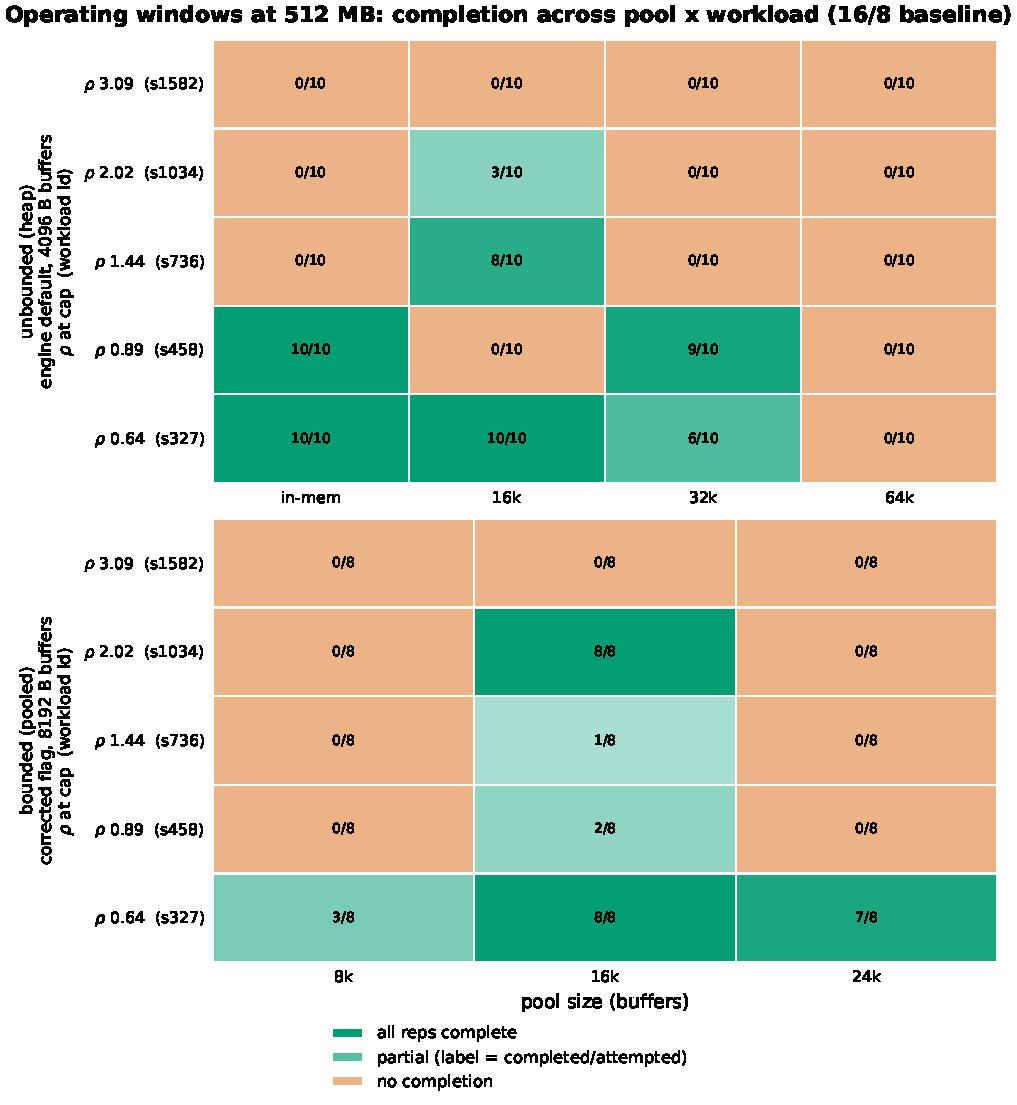
\includegraphics[width=0.72\textwidth]{img/fig_heatmap_512.pdf}
\caption[Operating windows at 512\,MB]{Operating windows at the 512\,MB cap
over pool $\times$ workload, 16/8 baseline only. State pressure $\rho$ (steady
footprint $\div$ cap; $\rho > 1$ = beyond memory) appears in parentheses; each
cell reports completed over attempted runs. Top panel: heap configuration
(engine-default, all window state outside the pool) with its capped in-memory
baseline; bottom panel: pooled configuration.
Figure~\ref{fig:geometry-law-512} breaks the failing bounded cells down by
failure reason; Figure~\ref{fig:tipping-point} isolates the heap configuration's s327 pool
sweep.\methodsnote}
\label{fig:heatmap-512}
\end{figure}

% [7.2.3d] 1024 MB: the two allocation types first differ in pattern.
At the mid-cap level (Figure~\ref{fig:heatmap-1024}), the two allocation types differ in pattern.
The completion of the bounded configuration increases with pool size in almost every row (s736: 0/8, 4/8, 8/8; s1582: 0/8, 0/8, 8/8).
The heap configuration has no such column order; s458 completes 10 of 10 at 32k, but 2 of 10 at 16k, and s1034 completes only at the largest pool.

One row, b1374, completes under neither allocation type at any pool.
Its state pressure ($\rho \approx 1.34$) is lower than s1582's ($\rho \approx 1.54$), which completes 8 of 8, so b1374 drives less total state than a workload that completes.
b1374 fails because of its pool demand rather than its total footprint.
Every bounded failure in this row is a pool-exhaustion abort, including at the largest pool tested; its concurrently live state requires a 96k-buffer pool ($\approx 786$\, MB), and a pool of that size cannot fit under a 1024\, MB cap alongside the state outside the pool.

\begin{figure}[htbp]
\centering
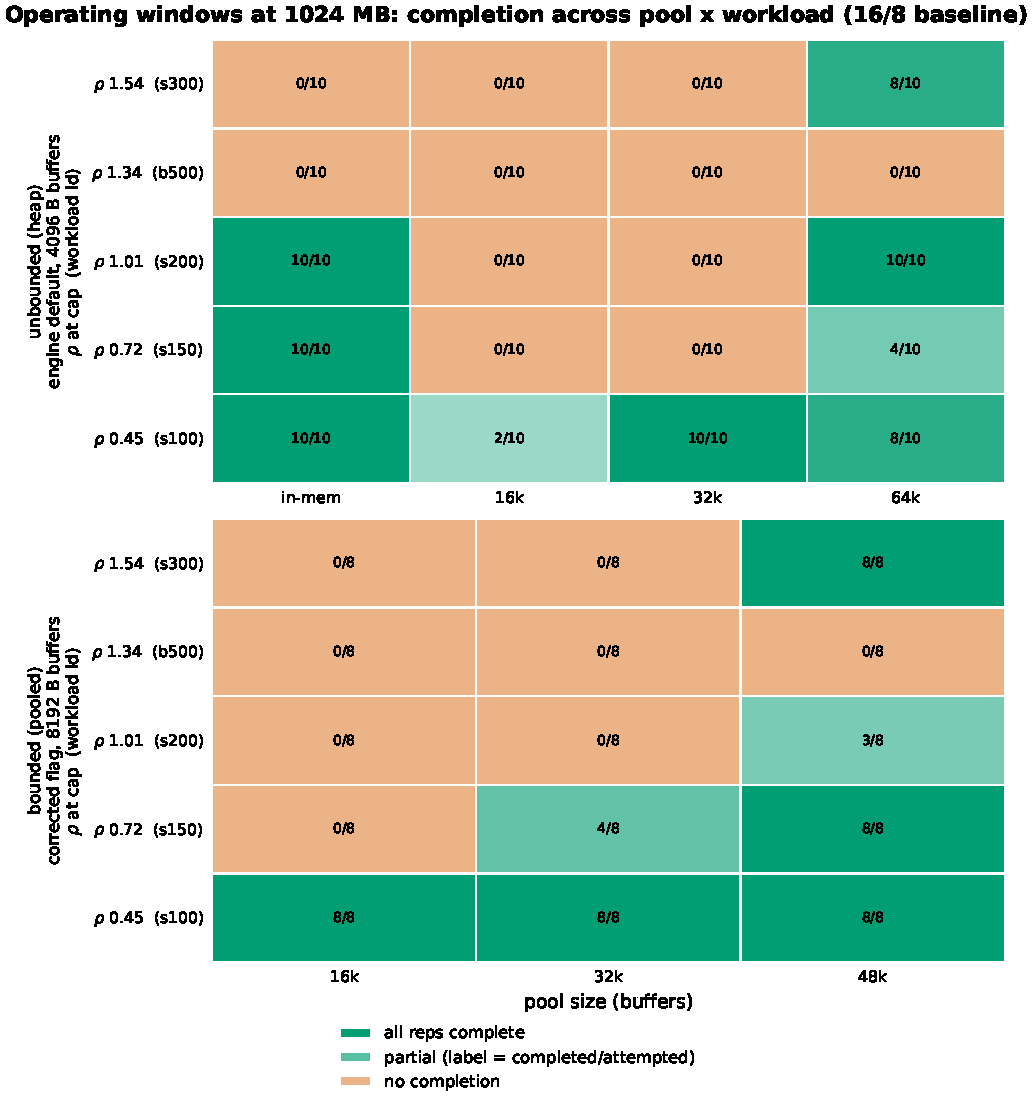
\includegraphics[width=0.72\textwidth]{img/fig_heatmap_1024.pdf}
\caption[Operating windows at 1024\,MB]{Operating windows at the 1024\,MB cap,
same layout as Figure~\ref{fig:heatmap-512}.\methodsnote}
\label{fig:heatmap-1024}
\end{figure}

% [7.2.3e] 2048 MB: bounded completes at the large-pool edge, heap in shifting bands.
At the largest cap (Figure~\ref{fig:heatmap-2048}) the bounded pattern continues.
Completion occurs only at the largest pools (s1034 from 64k, the rest at 96k), and no smaller pool completes anything.
b2078 ($\rho \approx 1.01$) completes nowhere, and every one of its bounded failures is a pool-exhaustion abort even at 96k, so the tested pools never reach its abort edge; whether a still larger pool would complete it under this cap is untested.

The heap configuration shows no single-column completion.
Each workload completes in its own narrow pool band (b1676 at 16k--32k, b1374 at 32k--64k, s1034 at 64k--128k), and the band shifts toward smaller pools as the workload's heap-resident state grows, because the pool is a fixed up-front reservation that competes with that state for the cap (Section~\ref{sec:rq1-geometry} isolates this mechanism).
No single heap pool column completes more than two of the five workloads, where the bounded 96k column completes four.
The exception to the band pattern is s1582, which completes nowhere on the heap although workloads with larger footprints do.
Section~\ref{sec:rq1-race} explains this exception through the ingest-drain race.

\begin{figure}[htbp]
\centering
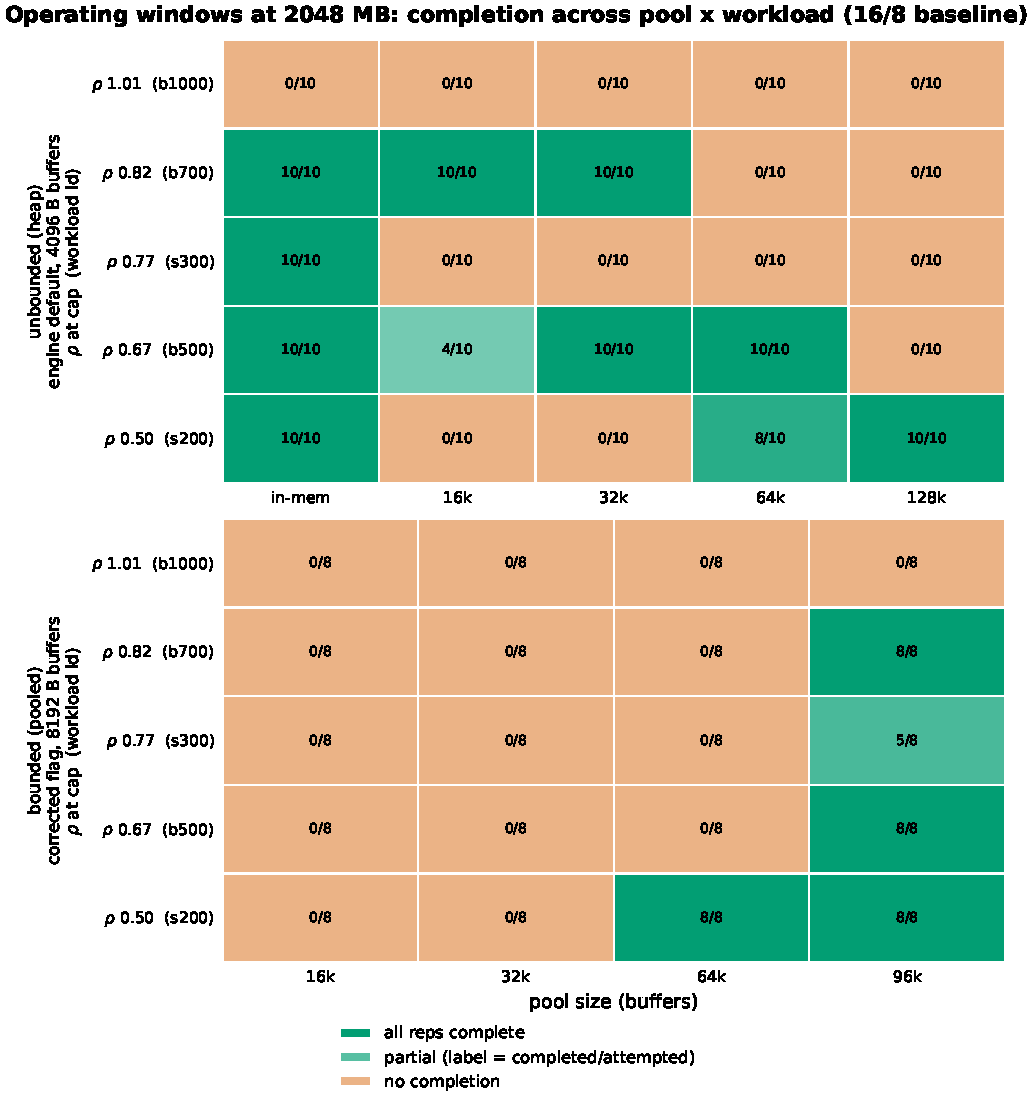
\includegraphics[width=0.72\textwidth]{img/fig_heatmap_2048.pdf}
\caption[Operating windows at 2048\,MB]{Operating windows at the 2048\,MB cap,
same layout as Figure~\ref{fig:heatmap-512}.\methodsnote}
\label{fig:heatmap-2048}
\end{figure}

\FloatBarrier
\subsection{The Two-Sided Geometry of the Bounded Window\label{sec:rq1-geometry}}

% [7.2.4] Two-sided geometry law; the per-cell failure breakdown is in sec:geometry-valley.
The pooled configuration's window depends on the pool geometry rather than on $\rho$.
The geometry has two bounds.
The lower bound is that the pool must hold the hot band of slices, the roughly $N_w$ windows that are concurrently open at any moment.
When the pool cannot supply this hot band, a worker's buffer request finds the pool empty, and NebulaStream aborts that allocation (Section~\ref{sec:backpressure}), thereby ending the run.
The upper bound is that the pool plus the overhead it induces must fit under the cap.
Every resident slice carries directory bytes outside the pool, so memory incurs a fixed per-slice cost decided at slice creation rather than one that scales with the pool's own size, and once the total exceeds the cap, the run is OOM-killed.
The two bounds therefore separate the two failure modes: a pool below the lower bound aborts, and a pool above the upper bound is OOM-killed.
Section~\ref{sec:geometry-valley} reads the failing cells of all three caps against these two bounds, failure mode by failure mode.


% [7.2.4b] The heap configuration's pool sensitivity, isolated at one cell.
The heap configuration is sensitive to the same knob.
The pool is a fixed slab that the engine reserves at process start, regardless of whether hash-map pages live in it (Section~\ref{sec:bg-nes}); growing it increases that up-front reservation and leaves less of the cap for the heap-resident window state, whose pages never enter the pool.
At 512\, MB, s327, the pool is the only variable, and completion falls from 10 of 10 at a 16k-buffer pool through 6 of 10 at 32k to 0 of 10 at 64k; every failure is an OOM kill.
Figure~\ref{fig:tipping-point} visualizes this sensitivity to pool size.

\begin{figure}[htbp]
\centering
\widefig{img/fig_tipping_point.pdf}
\caption[Pool-size sensitivity of the heap configuration]{Pool-size
sensitivity of the heap configuration at the 512\, MB cap, workload s327
($\rho \approx 0.64$); bars are completed/attempted per pool size, the only
variable tested here.\methodsnote}
\label{fig:tipping-point}
\end{figure}

\FloatBarrier
\subsection{Where Each Allocation Type Completes\label{sec:rq1-division}}

% [7.2.5]
At geometry-correct pools of roughly 40\% of the cap, the pooled configuration covers nearly the full default-configuration window at the larger caps.
It also adds cells that no heap variant completes.
At 2048\,MB, the pooled configuration completes the s1034 through b1676 workloads, with s1582 marginal at 5 of 8; that cell (s1582, 96k pool) is bounded-only, since both heap configurations complete 0 of 8 there.
At 1024\, MB, s736 and s1582 complete 8 of 8.
At 512\, MB, the upper bound sits below the hot band of the beyond-memory workloads, so only fitting and throttled workloads complete.
This small-cap limit is structural rather than a tuning artifact; it follows from the two bounds above.

% [7.2.5b]
The two allocation types divide the operating range.
Only the heap configuration completes at the 512\,MB cap and at cells whose unthrottled demand exceeds the storage-bandwidth ceiling of Section~\ref{sec:rq1-race} (s736 at the 512\,MB cap and 16k pool: heap 8 of 10, pooled 1 of 8), and it reaches higher throughput at the highest tested pressures, where the pooled configuration loses time to allocation stalls on the shared pool (Section~\ref{sec:rq4}).
The pooled configuration provides the footprint guarantee, the bounded-only cells, and graceful degradation.
One workload marks the absolute edge; b2078 at 2048\, MB ($\rho \approx 1.01$) fails under every configuration tested.

Table~\ref{tab:windows} summarizes the operating windows.

\begin{table}[ht]
\centering
\small
\begin{tabular}{|p{1.5cm}|>{\raggedright\arraybackslash}p{5.1cm}|>{\raggedright\arraybackslash}p{5.1cm}|}
\hline
\textbf{Cap} & \textbf{Heap (unbounded allocation)} & \textbf{Pooled (bounded allocation)} \\
\hline
512\,MB  & $\rho \approx 1.2$--$2.2$ \newline (s736: 8/10 vs 0/10, $p=3.6\times10^{-4}$) & fits + throttled $\rho\approx2$ \newline (s1034: 8/8 vs 0/10, $p=2.3\times10^{-5}$) \\
\hline
1024\,MB & up to $\rho = 1.54$, largest tested \newline (s1582: 8/10 vs 0/10, $p=3.6\times10^{-4}$) & s736 and s1582, 8/8 each \newline (48k-buffer pool) \\
\hline
2048\,MB & below $\rho \approx 1$ \newline (b1374/b1676 10/10; no spill) & s1034--b1676 at the 96k pool \newline (s1582 5/8, pooled-only; heap 0/8) \\
\hline
\end{tabular}
\caption[Operating windows by cap and allocation type]{Demonstrated operating windows per cap and allocation type, with the
headline evidence in parentheses. Heap columns are the engine-default
configuration (4096-byte buffers; all window state on the heap,
Section~\ref{sec:integration}); pooled columns are the 8192-byte configuration
that engages pooling. Beyond the memory boundary at 2048\,MB nothing is
demonstrated: b2078 ($\rho \approx 1.01$) fails under every configuration.}
\label{tab:windows}
\end{table}

% [7.2.6c] Multi-cap completion headline (generalizes the 512\,MB flagship).
Figure~\ref{fig:effectiveness} shows the table's headline in two panels.
Panel (a) isolates the baseline; no capped in-memory cell completes once state clearly exceeds memory.
One baseline cell, s1034 at 1024\, MB, completes 10 of 10 although its uncapped $\rho$ is 1.01, because the uncapped reference run, under no page reclaim pressure, uses about ten percent more memory than the same workload under the cap; the capped peak is 948\, MB and fits under 1024\, MB.
Panel (a) therefore plots this cell at its realized capped pressure ($\rho \approx 0.93$).
The contrast is b2078 at 2048\, MB, which has the same uncapped $\rho \approx 1.01$ but exceeds its cap in capped execution as well and fails 0 of 10.

Panel (b) compares the two configurations at and beyond the boundary; the lighter workloads, which both configurations complete in full, are omitted there because Figures~\ref{fig:heatmap-512}--\ref{fig:heatmap-2048} show the full grids.
At 512 and 1024\, MB, the best \ac{OOC} operating point, taken over pool sizes and both allocation types, extends completion past the memory boundary.

One cell in panel (b) breaks the left-to-right order of $\rho$.
b1374 at 1024\,MB ($\rho \approx 1.34$) fails on both configurations because its required pool does not fit under the cap (Section~\ref{sec:rq1-windows}), while s1582 immediately to its right ($\rho \approx 1.54$, a larger footprint) completes 8 of 8 \ac{OOC} through a 48k pool that does fit; the figure's tag for this bar (64k, heap) names the largest pool actually tested at this cap.
Completion therefore depends on whether the required pool fits within the cap, and the total footprint is not the determining factor.
At 2048\, MB, the single beyond-memory workload, b2078 at $\rho \approx 1$, fails under every configuration; completion beyond the memory boundary is therefore demonstrated at the 512 and 1024\,MB caps only.

\begin{figure}[htbp]
\centering
\widefig{img/fig_effectiveness.pdf}
\caption[Completion at the memory boundary]{Completion at the memory
boundary. (a) The capped in-memory baseline per cap and workload, labeled
completed/attempted (green = all complete, orange = partial, red = all fail).
(b) The capped baseline against the best \ac{OOC} operating point per cell
($\rho \geq 0.75$); tags name each point's pool size and allocation type
(H = heap, B = bounded); shaded spans mark the beyond-memory
pairs.\methodsnote}
\label{fig:effectiveness}
\end{figure}

\FloatBarrier
\subsection{Completion as a Race\label{sec:rq1-race}}

% [7.2.6]
Completion does not depend on state pressure alone.
Under the heap configuration, a workload at $\rho \approx 0.77$ ingesting 2.8 million tuples per second fails (s1582 at 2048\, MB, the empty row of Figure~\ref{fig:heatmap-2048}).
A heavier workload at $\rho \approx 0.82$ ingesting 1.1 million tuples per second completes 10 of 10 (b1676, the row above it).
The lighter workload fails, and the heavier one completes, so the outcome depends on the ingest rate rather than on the footprint.

% [7.2.6b] C18: the non-monotone completion, both mechanisms + n=8 / CI caveat.
Under the pooled configuration, the same reversal appears within one cap.
At 512\,MB with a 16k-buffer pool, completion is non-monotone as $\rho$ rises, 8/8, then 2/8, then 1/8, then 8/8 (the middle column of Figure~\ref{fig:heatmap-512}, bottom panel).
Two mechanisms produce this shape.

The first mechanism is the fast-ingest valley, and it explains why the heaviest load completes again after the lighter ones fail.
At the lower $\rho$ points, the working set fits, so the pool fills late or not at all, and the sources are not throttled.
The workload runs unthrottled above the storage-bandwidth ceiling of about 2.6 million tuples per second, the spiller falls further behind with every window, and the run fails.
At the heaviest point ($\rho \approx 2$) the per-window state is large enough that the pool is full early in the run.
From then on, every allocation waits for a freed buffer, and buffers are freed at the rate the spiller writes to the device, so ingest is forced down to the storage-bandwidth rate; the run finishes slowly instead of failing fast.
More state pressure, therefore, restores completion because it engages this throttling from the start, while middle workloads run unthrottled past the ceiling.
The measured rates confirm this; the completing run ingests about 1.98 million tuples per second, where the fast failures run unthrottled at about 3.33 million.

The second mechanism is small-sample variance.
Each cell rests on only eight repetitions, so an exact fraction carries a wide confidence interval; 8/8 spans a 95\% Wilson interval of 68 to 100 percent, and 2/8 spans 7 to 59 percent.
The same cell rerun under the 32/32 backend configuration of \hyperref[app:rb32]{Appendix~E.6} completes 6 of 8 rather than 2 of 8, inside that interval.
The mechanism is robust, while the exact fractions carry wide intervals (Section~\ref{sec:threats}).

% [7.2.6c] The three valley figures: the curve, the mechanism, the run-time view.
Figures~\ref{fig:valley}, \ref{fig:pacing-loop}, and \ref{fig:throttle-trace} show this at the 512\,MB cap and 16k pool.
Figure~\ref{fig:valley} plots the completion valley against the naive expectation that completion tapers with size, and marks each failing cell by its cause.
The valley also shows both failure types of the sizing law (Section~\ref{sec:rq1-geometry}).
The lighter middle workloads abort because the fixed pool cannot hold their concurrently live band, while the heaviest workload is OOM killed because its resident state leaves no headroom under the cap for the rest of the engine.
Pacing recovers completion only within the band between these two edges; a pool too small to hold the live band aborts, and state too large to leave headroom is OOM-killed, however slowly the sources are fed.

\begin{figure}[htbp]
\centering
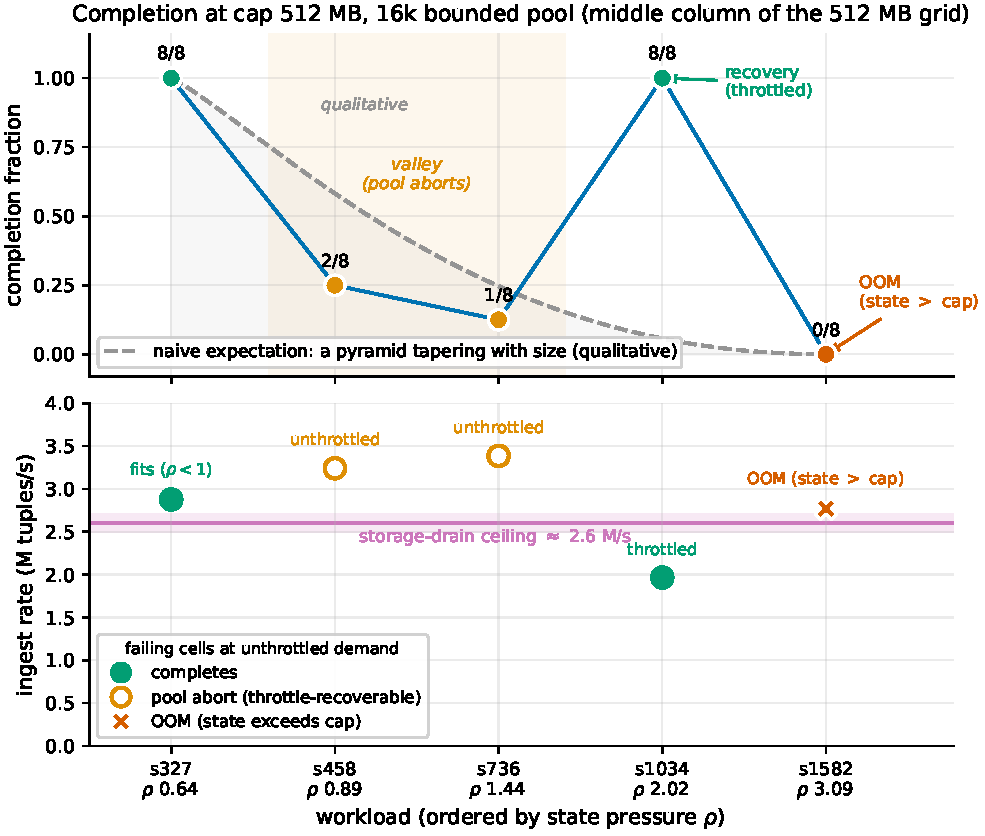
\includegraphics[width=0.82\textwidth]{img/fig_valley.pdf}
\caption[The completion valley at 512\,MB]{The completion valley at the
512\, MB cap and 16k bounded pool: completion fraction (top) against the naive
tapering expectation (dashed, qualitative rather than a fitted model), and ingest
rate (bottom) against the storage-drain ceiling, both ordered by state
pressure $\rho$. Failing cells are plotted at their unthrottled demand, since
a failed run has no realized rate of its own.\methodsnote}
\label{fig:valley}
\end{figure}

The throttle behind this recovery is the engine's bounded admission queue (Figure~\ref{fig:pacing-loop}).
The queue mechanism exists verifiably in the engine.
Work is admitted through a bounded queue (default 1000 tasks, \texttt{admission\_queue\allowbreak\_size}), and a source that finds the queue full blocks in \texttt{addAdmission\allowbreak Task\allowbreak Blocking}, retrying in timed intervals, so its thread sleeps until a slot frees.
Buffers return only as fast as the spiller writes to the device, task consumption slows, the queue fills, the sources sleep, and ingest is forced down to the storage-bandwidth rate.
How much each stage of this chain contributes to the observed slowdown remains a hypothesis, because the probes record no per-thread scheduling; measuring the chain end-to-end requires scheduler-level instrumentation, which is left as future work.


\begin{figure}[htbp]
\centering
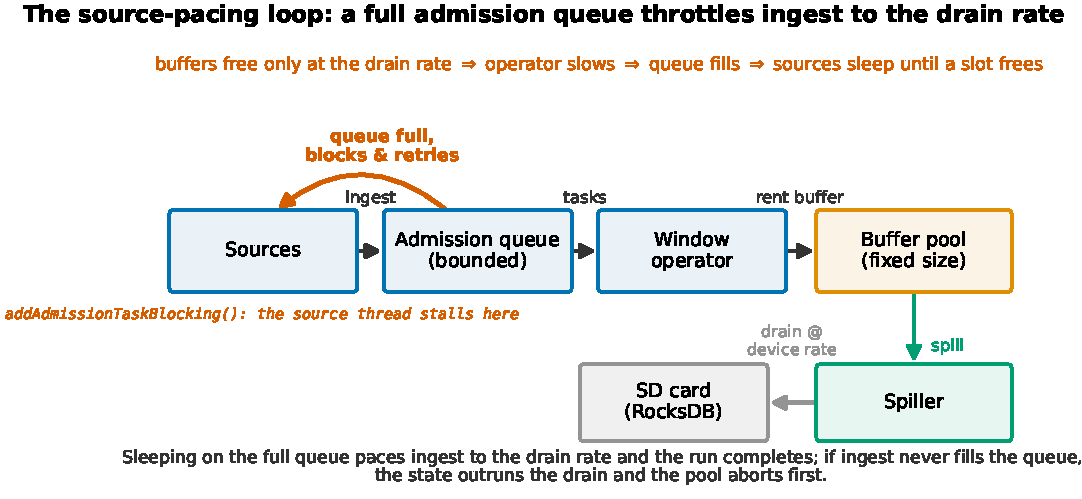
\includegraphics[width=0.85\textwidth]{img/fig_backpressure_loop.pdf}
\caption[The source-pacing loop]{The pacing loop behind the valley (conceptual
diagram, no measured data). The diagram shows the engine's intrinsic queue
pacing rather than the allocation-backpressure lever of
Section~\ref{sec:backpressure}, which was tested separately and refuted.}
\label{fig:pacing-loop}
\end{figure}

Figure~\ref{fig:throttle-trace} shows the same runs over their lifetimes; the paced heaviest workload maintains a bounded working set throughout the run, while the lighter loads abort early.
The trace also separates the two memory quantities the outcome depends on.
The total accounted memory, including the page cache, remains at the cap in every spilling run and causes no failures; this is the page-reclaim-held plateau introduced in Section~\ref{sec:bg-metrics}.
The OOM kill is triggered by the anonymous set alone when it grows beyond what the kernel can reclaim.
In the figure, the dashed totals plateau at 511 or 512\, MB because samples round to either side of the byte-precise cap; true usage never exceeds the cap by more than a fraction of a megabyte (Section~\ref{sec:bg-metrics}).

\begin{figure}[htbp]
\centering
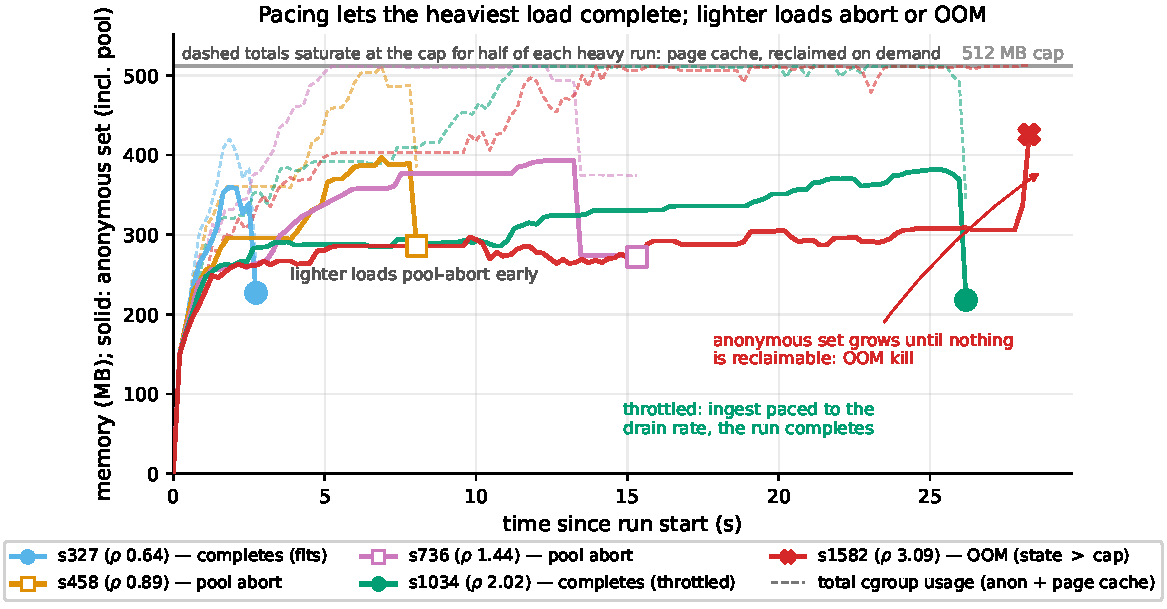
\includegraphics[width=0.95\textwidth]{img/fig_throttle_trace.pdf}
\caption[The throttle over one run's lifetime]{The valley mechanism in time.
Solid lines show the anonymous working set (pool reservation, unpooled window
state, and engine overhead); thin dashed lines show total accounted cgroup
memory (anonymous set plus page cache). One run per workload at the 512\, MB
cap and 16k pool; end markers and the legend give each run's
outcome.\methodsnote}
\label{fig:throttle-trace}
\end{figure}

% [7.2.7]
Completion is therefore a race between the ingest rate and the rate at which the spiller drains state to disk.
Figure~\ref{fig:race} plots this race, one point per spilling cell, ingest rate against state pressure.
A completing cell is plotted at its realized ingest rate; a failing cell is plotted at the workload's unthrottled demand, the rate it reaches unconstrained, because a failed run has no realized rate of its own.
The $\rho = 1$ boundary in the figure is exact by definition.
The storage-bandwidth ceiling near 2.6 million tuples per second is empirical; it is the highest throughput any completing spilling cell realizes, and no $\rho > 1$ cell whose demand exceeds about 2.7 million tuples per second completes (25 of 25 fail).
Above the boundary and to the right of the ceiling, the ingest exceeds the drain rate, and the run fails.
The rest of the chapter builds on this framing.

\begin{figure}[htbp]
\centering
\widefig[1.0]{img/fig_race.pdf}
\caption[Completion as a race between ingest and drain]{Completion as a race
between ingest and drain, one point per cell of both grids. Color and shape
give the outcome (green circle = completes, orange square = pool-exhaustion
abort, red cross = OOM kill); fill gives the allocation type (filled = heap,
hollow = bounded). The horizontal line marks the $\rho = 1$ memory boundary,
the vertical line the storage-bandwidth ceiling near
2.6\,M tuples/s.\methodsnote}
\label{fig:race}
\end{figure}

% [7.2.7b] The two rho<1 failure groups, compressed: both recover at the
% geometry-correct pool, so both are pool-geometry effects.
Below $\rho = 1$ the workload fits in memory, and the capped in-memory baseline completes every such cell.
The out-of-core backend fails 33 of these fitting cells, 24 by pool-exhaustion abort and 9 by OOM kill, because the tested pool was mis-sized; the plain in-memory engine has no pool and therefore no such failures.
These failures fall within the two bounds of Section~\ref{sec:rq1-geometry}, and all of them recover in the geometry-correct pool, so none of them are due to insufficient memory.
The one partial recovery is s1582 at 2048\, MB, whose unthrottled demand of about 2.8 million tuples per second exceeds the storage-bandwidth ceiling and which recovers only 5 of 8 at the best pool.
Above $\rho = 1$ the race sets the opposite edge; no cell whose demand exceeds the storage-bandwidth ceiling completes, because ingest exceeds the drain rate.

\FloatBarrier
\FloatBarrier
\subsection{Transfer to a Realistic Workload\label{sec:nexmark}}

% [7.2.8]
The synthetic grid is the primary evidence.
A Nexmark-style auction bid stream provides supporting evidence.
The stream uses the canonical bid schema, hot-skewed auction popularity, and in-order event time.
The configuration matrix mirrors the synthetic grid.

Two queries run. Both are pure tumbling-window aggregations, the operator whose state this backend spills.
\texttt{q3} computes the sum of bid prices per auction within each tumbling window; \texttt{q7}, Nexmark's \emph{Highest Bid}, computes the maximum bid per auction within each window.
They are chosen because aggregation is exactly the mechanism under test, and because the two differ only in the aggregate function, sum versus maximum.
Any difference between them, therefore, isolates the aggregate rather than the state machinery, so a matching result across both shows that the finding does not depend on any particular reduction.
Nexmark's join queries (for example q8) fall outside the tumbling-window scope of this thesis and are not run.

\paragraph{Methods note\label{sec:methods-nexmark}}
Every Nexmark figure in this chapter includes a short pointer back to this note rather than repeating the full setup under each plot.

\nexmarknotefull

Each query runs across three state scenarios, A, B, and C, that grow the per-window state by widening the window; A is the smallest, C the largest.
Each memory cap pairs one scenario the in-memory engine can hold with one that stresses it, A and B under the 512\, MB cap and B and C under the 1024\, MB cap.
Only the largest scenario at the larger cap, C at 1024\, MB, drives the window state past what the in-memory engine can fit; that single cell is the beyond-memory point, the coordinate where only \ac{OOC} processing completes the workload.
Each cell runs three configurations at eight repetitions: the capped in-memory engine, the bounded pooled backend (B2: 15\% pool reserve, paced restore, soft and hard thresholds at one-tenth and one-fifth of the cap), and the heap \ac{OOC} backend (U8).

The purpose is external validity.
The synthetic grid is a single stream shape, generated with out-of-order jitter; a canonical benchmark with a different schema, hot-skewed auction popularity, and an in-order event stream tests whether the result holds beyond the conditions under which it was measured.
The bounded backend completes this workload where the capped in-memory engine cannot, 8 of 8 and 7 of 8 versus 0 of 8 ($p = 7.8 \times 10^{-5}$ and $7.0 \times 10^{-4}$).
The runs performed verified \ac{OOC} work, 610\, MB spilled and 234\, MB restored from the device.
Figure~\ref{fig:nexmark-sweep} places this result in context across scenarios and caps; the capped in-memory engine fits the small and medium scenarios and fails only at the beyond-memory point at 1024\, MB, which is where the bounded backend completes.

\begin{figure}[htbp]
\centering
\widefig[0.9]{img/fig_nexmark_sweep.pdf}
\caption[Nexmark completion across scenarios and caps]{Nexmark completion
across scenarios and caps for queries q3 and q7. Bars are completion fraction
(completed over attempted, labeled) for the capped in-memory engine, the
bounded \ac{OOC} backend, and the heap \ac{OOC} backend.\nexmarknote}
\label{fig:nexmark-sweep}
\end{figure}

% [7.2.8b] The fits-cell failure under the fixed threshold; q3-vs-q7 compressed.
The same figure shows both \ac{OOC} configurations failing at a cell the in-memory engine completes.
In scenario B, under the 512\,MB cap for q7, the capped in-memory engine completes 8 of 8, while both \ac{OOC} configurations complete 0 of 8, even though the state fits within 512\,MB.
The cause is the fixed cap-derived spill threshold, set to 1/10 of the cap.
It fires on the cap alone, without measuring how much of the cap the state occupies, so it spills here, even though nothing needs to spill.
The one-tenth fraction is not independently tuned; the cap-derived rule outperformed the pool-derived rule at a single cell, 512\,MB cap and 16k pool with s1034 (Section~\ref{sec:rq3}), and the exact fraction was not swept further.
At the tight 512\, MB cap, this over-spilling produces a different failure in each configuration; the pooled configuration's small pool, about 125\, MB at this cap, exhausts and aborts (exit code 141), while the heap configuration's unpooled buffers exceed the cap and are OOM killed (exit code 137).

On q3, the same cell retains a few repetitions (bounded: 5 of 8, heap: 1 of 8); this single q3-versus-q7 discrepancy is boundary sensitivity at a cell where both queries barely pass or already fail, since both aggregates keep one accumulator per key and carry identical state.
The headline coordinate, C at 1024\, MB, is unaffected; there the in-memory engine cannot fit the state (0 of 8) and the bounded backend completes (q7 7 of 8, q3 8 of 8).

% [7.2.8c] The two OOC configurations are not interchangeable; the trade-off reverses across the sweep.
The two \ac{OOC} configurations are not interchangeable, and the trade-off between them reverses across the sweep.
On the fitting cells that over-spill but keep memory headroom under the cap (scenario A at 512\, MB and scenario B at 1024\, MB), the heap configuration completes every run (8 of 8 on all four query--cell combinations), because the unnecessary spilling costs it throughput but no memory.
The bounded configuration is limited by its own fixed pool (125\, MB at the 512\, MB cap, 375\, MB at 1024\, MB); the spill-and-restore churn saturates the pool and completion falls to between 2 and 6 of 8, lowest at q3 scenario B under 1024\, MB (2 of 8 against the heap configuration's 8 of 8).
On these cells, the fixed pool is the binding constraint, and heap allocation completes more runs.
At the one tight-fitting cell, scenario B at 512\, MB, the same over-spilling fails both configurations through their respective failure modes, the pool abort and the OOM kill, as above.

The ordering reverses at the one-beyond-memory coordinate, C at 1024\,MB, where the in-memory engine cannot fit the state (0 of 8), and spilling is required.
There, the bounded configuration's pool-bound and paced restore keeps total memory under the cap and completes most reliably (q3 8 of 8, q7 7 of 8), while the heap configuration's unbounded restore intermittently exceeds the cap and is OOM-killed, completing 6 of 8 and 3 of 8.
This coordinate is the deployment case that motivates the backend, and only the pooled configuration completes it reliably.

% [7.2.9]
The same runs test the failure model on data it was not built from; both of its components, the geometry law (Section~\ref{sec:rq1-geometry}) and the slice-cache corruption (Section~\ref{sec:rq3}), were derived on the synthetic grid alone.
The corruption mechanism requires late writes, and the in-order stream has none, so the model predicts zero corruption events; zero occur in the 210 Nexmark runs.
Every bounded failure occurs at the pool size the geometry law predicts.


% [7.2.11] --- answer to RQ1
In answer to RQ1, the backend prevents the OOM failure the capped in-memory engine suffers, within a characterized window rather than unconditionally; the two-sided pool geometry and the ingest-drain race bound that window, and Table~\ref{tab:windows} states it per cap and allocation type.
The result transfers beyond the synthetic grid; on a realistic Nexmark bid stream at its one beyond-memory coordinate (scenario C at 1024\,MB), the bounded backend completes where the capped in-memory engine cannot (q3 8 of 8 and q7 7 of 8 versus 0 of 8; Figure~\ref{fig:nexmark-sweep}).
The next section investigates why the remaining failures happen and which mechanism this completion is attributed to.

\section{Memory Behavior and Stability (RQ3)\label{sec:rq3}}

RQ3 asks how memory behaves as state grows past the cap, and why the remaining failures happen.
This section reports the allocation finding (C4) and the failure taxonomy (C5), the investigation whose products, the two-sided geometry and the ingest-drain race, the previous section used to map the operating windows.
The steps appear in the order the experiments were run because the sequence of refuted hypotheses constitutes the evidence for the final explanation; every hypothesis was pre-registered before its run.

% [7.6a]
The two constraints of Section~\ref{sec:rq1-geometry} form a feasibility corridor per cap and workload, and the corridor is narrow; at the s327 cell of Figure~\ref{fig:tipping-point}, pools of 16k and 32k buffers complete while the 64k pool fails.

% [7.6b]
Where the backend completes, it uses 14--22\% less anonymous memory than the in-memory engine on identical workloads.
The reason is that pooled pages return to the pool on spill and are reused.
The advantage grows as the pool shrinks.

% [7.6c]
The four pool-pressure levers (Section~\ref{sec:levers}) executed their spills as designed but converted no failing cell.
The initial conclusion was that the resident memory is a minimum and cannot be spilled.

% [7.6d]
This conclusion was wrong, because the levers never acted on window state.
The engine's 4096-byte default buffer size (Section~\ref{sec:integration}) kept every map page out of the pool in every prior experiment, so the pool contained no window state.
The conclusion was retracted.

% [7.6e]
One flag (buffer size 8192) engages the intended memory configuration; Figure~\ref{fig:ladder} shows the resulting completion counts.

The baseline completes 0 of 10.
(A further configuration, matched buffer size without pooling, recovers 3 of 8; it appears as the second rung of Figure~\ref{fig:ladder}, and its effect is separated from the allocation type below.)
Levers without pooling complete 0 of 16.
Pooling without levers completes 0 of 8.
Pooling with the reserve lever (Lever 1a) completes 5 of 8.
Pooling with the reserve lever and paced restore (Lever 1c) completes 7 of 8; within pooling, the levers carry the cell from 0 of 8 to 7 of 8 ($p = 7.0 \times 10^{-4}$).
Taken together, the pooled lever configurations complete 12 of 16, whereas levers without pooling complete 0 of 16 ($p = 8.1 \times 10^{-6}$).

\begin{figure}[htbp]
\centering
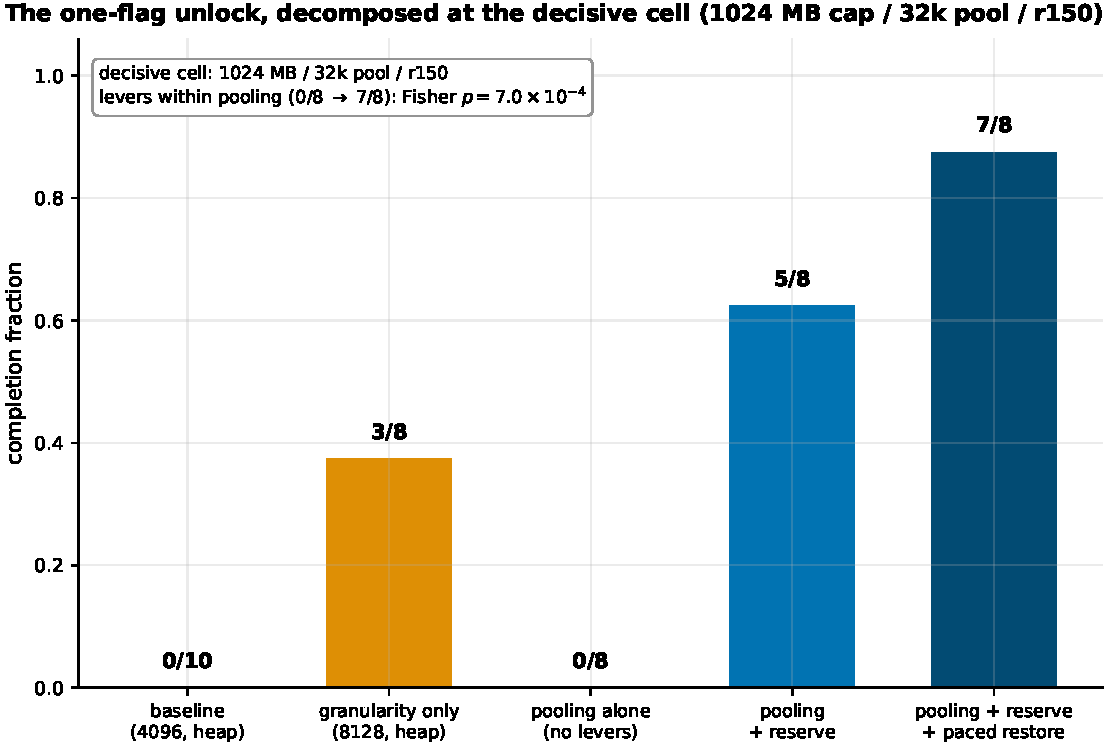
\includegraphics[width=0.85\textwidth]{img/fig_ladder.pdf}
\caption[The attribution ladder]{The attribution ladder at the cell
1024\,MB / 32k pool / s736. Bars show completed/attempted per
configuration, each changing exactly one factor from the baseline. The
buffer-size-alone configuration uses 8128-byte buffers, just under the
8192-byte page, so map pages stay on the heap
(Section~\ref{sec:disambiguation}).\methodsnote}
\label{fig:ladder}
\end{figure}

% [7.6f]
At the 1024\,MB cap with a 32k pool and s736, under pooling with reserve and paced restore, the backend reaches 98\% of the in-memory engine's throughput (3.38 versus 3.44 million tuples per second).
It uses 25\% less anonymous memory, 517 versus 685\, MB.
Its 99th-percentile latency is 2.2 times higher.

% [7.6h]
Pooling changes the sizing rules.
Because the up-front pool reservation sets the minimum anonymous memory of a run (Section~\ref{sec:rq1-geometry}), a smaller pool reduces the footprint and, at the same time, increases completion, as long as it still holds the hot band; choosing the pool size no longer forces a choice between footprint and completion.

% [7.6i]
Three alternative explanations for the remaining failures were pre-registered and refuted.
Deriving the soft threshold from the pool rather than the cap results in 0 of 8 everywhere.
Bounding source admission changes nothing.
Bounding the task queue changes nothing; the queue throttles ingest and does not free memory.

% [7.6j]
Allocation backpressure (Section~\ref{sec:backpressure}) also converted nothing.
Its instrumentation provided the diagnosis instead.
In 118 of 138 stalls, no buffer returned anywhere in the pool for two full seconds.

% [7.6k]
The residual failure is an allocation deadlock (Figure~\ref{fig:gridlock}).
Emitted but unprocessed window state holds the pool's buffers.
Draining that state back out requires worker threads.
Every worker thread is itself blocked waiting to allocate.
The pool has no separation between fill-side and drain-side allocations, so fill-side allocations consume the buffers the drain side needs.

\begin{figure}[htbp]
\centering
\widefig{img/fig_gridlock.pdf}
\caption[The allocation deadlock]{The allocation
deadlock at a failing allocation-backpressure cell (1024\, MB / 32k pool /
s1034, all eight repetitions fail by allocation abort). (a) The 0.2-second
memory sampler of one repetition; the working set rises until no worker can
allocate. (b) Pool occupancy at its peak and at process death across all
repetitions; the pre-allocated pool is 250\,MB.\methodsnote}
\label{fig:gridlock}
\end{figure}

% [7.6l]
The results compose into a three-regime feasibility law (Figure~\ref{fig:regimes}), which joins the pool geometry of Section~\ref{sec:rq1-geometry} to the race of Section~\ref{sec:rq1-race}.
In regime one, the demand fits the pool, and the run completes at full speed.
In regime two, the demand exceeds the pool, but the memory cap throttles ingest, and the run completes at reduced speed.
In regime three, the demand exceeds the pool, ingest is unconstrained, and the run deadlocks.
The evidence for the two boundaries lies in the preceding results: the pool geometry separates regime one from the rest (Section~\ref{sec:rq1-geometry}), and the valley column contrasts regimes two and three at a single cap, pool, and configuration (Section~\ref{sec:rq1-race}).
One workload appears on both sides of the second boundary: s1034 completes throttled at the 512\,MB cap and 16k pool, paced to the drain rate, and deadlocks at the 1024\,MB cap and 32k pool (Figure~\ref{fig:gridlock}).
The two cells differ in cap, pool, and lever configuration, so this pair illustrates the regimes rather than isolating what separates them.
Regime two's throttling is the admission-queue pacing of Section~\ref{sec:rq1-race}.

\begin{figure}[htbp]
\centering
\widefig{img/fig_regimes.pdf}
\caption[The three-regime feasibility law]{The three-regime feasibility law.
Starred points mark the same-workload contrast pair discussed in the text
(s1034 at the 512\, MB cap versus the 1024\, MB cap).\methodsnote}
\label{fig:regimes}
\end{figure}

% [7.6m]
The recommended operating configuration is pooling with reserve and paced restore, allocation backpressure off.
The allocation-backpressure lever reduces throughput by 10\% near the small-pool edge of the operating window and converts nothing.

% [7.6n]
The full-grid confirmation run answers three open questions.
The soft threshold must stay cap-derived; at the 512\,MB cap with a 16k pool and s1034, the pool-derived rule completes 3 of 8 against the cap-derived rule's 8 of 8 (Fisher's exact test, $p = 0.026$), confirming in direction the falsification arm above.
A memory-corruption crash cluster appears at high-churn cells (root-caused in Section~\ref{sec:geometry-valley}).
The two allocation types' windows are complementary, and the allocation deadlock is the demonstrated reason the pooled window cannot widen; a pool that reserves buffers for the drain side that the fill side cannot consume is the only mechanism that would merge the two windows.

\FloatBarrier
% [7.6o–q] The flag's two effects, separated (dissolved subsection).
One check remains before the failure analysis.
The one-flag change behind Figure~\ref{fig:ladder} alters two things at once, the allocation type and the I/O buffer size, so every result above could in principle be a buffer-size effect; a dedicated control configuration separates the two.\label{sec:disambiguation}
Its buffer size of 8128 bytes is 99.2\% of the page size but still below it; because a page is pooled only when it fits inside the buffer (Section~\ref{sec:integration}), maps stay on the heap at the matched buffer size, so any remaining difference against the pooled configuration is due to the allocation type alone.

Two results confirm the allocation type as the cause.
The $\rho \approx 2$ completion at 512\,MB (s1034, 16k pool) disappears without pooling; pooled completes 8 of 8 (the bottom panel of Figure~\ref{fig:heatmap-512}) and the matched-buffer-size heap 0 of 8 (Fisher's exact test, $p = 7.8 \times 10^{-5}$).
The lever effect also stands unchanged at fixed buffer size (0 of 8 to 7 of 8, $p = 7.0 \times 10^{-4}$; the third and fifth rungs of Figure~\ref{fig:ladder}), so it is not a buffer-size artifact.
Pooling is not uniformly ahead; at one 512\,MB cell (s736 at the 16k pool, $\rho \approx 1.44$), the matched-buffer-size heap completes 7 of 8 and pooled 1 of 8 (the same panel), and at the highest tested pressures only heap allocation completes (Figures~\ref{fig:heatmap-512}--\ref{fig:heatmap-2048}).

The buffer size's own effect cannot be fully separated at the 1024\,MB cap with a 32k pool and s736.
There, the buffer size alone recovers 3 of 8 from 0 of 10 ($p = 0.069$; the first two rungs of Figure~\ref{fig:ladder}), and the pooled-lever configurations (11 of 16 in the confirmation runs) sit directionally above the matched-buffer-size heap's 3 of 8 without being separable at this sample size ($p = 0.15$).
With the two effects separated, the remaining question is why the failing cells fail; the next subsection reads them against the two bounds.

\FloatBarrier
\subsection{Geometry, the Valley, and the Crash Cluster\label{sec:geometry-valley}}

% [7.6r-intro] Subsection opening: what it establishes, in order.
This subsection accounts for every remaining failure in the grids.
It shows that the bounded failures follow the two bounds of Section~\ref{sec:rq1-geometry} at every cap, that the fast-ingest valley recurs wherever the bounds permit completion, and that the crash cluster, the one failure class that is not a memory failure, is a slice-cache defect confined to cells that already fail.

% [7.6r]
The first bounded campaign at the 2048\,MB cap completed nothing; every tested pool size produced an all-zero column.
This was due to the pool geometry rather than the deadlock; the tested pool sizes lay on both sides of the working range and missed it.
A pool at 39\% of the cap, initially untested, completes s1034 through b1676 (the 96k column of Figure~\ref{fig:heatmap-2048}).

% [7.6s]
The geometry rule carries over across caps until the base footprint no longer fits beside the pool.
At 1024\,MB, the corresponding 48k pool ($\approx$39\% of the cap) completes two workloads that no smaller pool fully completes there, s736 and s1582 (8 of 8 each; Figure~\ref{fig:geometry-law-1024}).
At 512\,MB, the corresponding 24k pool ($\approx$39\% of the cap) is OOM-killed on every workload above s327 (Figure~\ref{fig:geometry-law-512}), because the directory overhead the pool induces exceeds the cap.
Figures~\ref{fig:geometry-law-512}--\ref{fig:geometry-law-2048} read the full grids against the two bounds, cap by cap.

Each cell in Figures~\ref{fig:geometry-law-512}--\ref{fig:geometry-law-2048} reports how many runs completed and how the rest failed.
Pool exhaustion aborts (exit code 141) occur at the small pool edge, where the pool cannot hold the hot slice band.
Memory-pressure failures (exit code 137 OOM kill, or exit code 134 allocator abort under the cap, counted together) occur at the large-pool edge, where the pool plus the unpooled directory bytes of each resident slice exceeds the cap.
The corruption segfaults root-caused below are counted separately as ``crash'' and appear only inside cells that fail regardless; cells whose repetitions mix failure modes are hatched and colored by the dominant mode, and the split is written on the cell.
The three caps show the two bounds in complementary partial views.

At 512\, MB both edges of the law are visible (Figure~\ref{fig:geometry-law-512}).
At the small pool (8k) the lighter workloads abort; s327 completes 3 of 8, while s458 and s736 abort in full.
The two heaviest rows are already past the OOM edge at this pool size, with s1034 and s1582 failing 0 of 8 due to OOM.
The middle pool (16k) holds every full completion, the fitting s327 and the throttled s1034, both 8 of 8.
At the large pool (24k) every workload above s327 is OOM killed; the one mixed cell is s1582 at 24k (6 OOM, 1 timeout, 1 crash).

\begin{figure}[htbp]
\centering
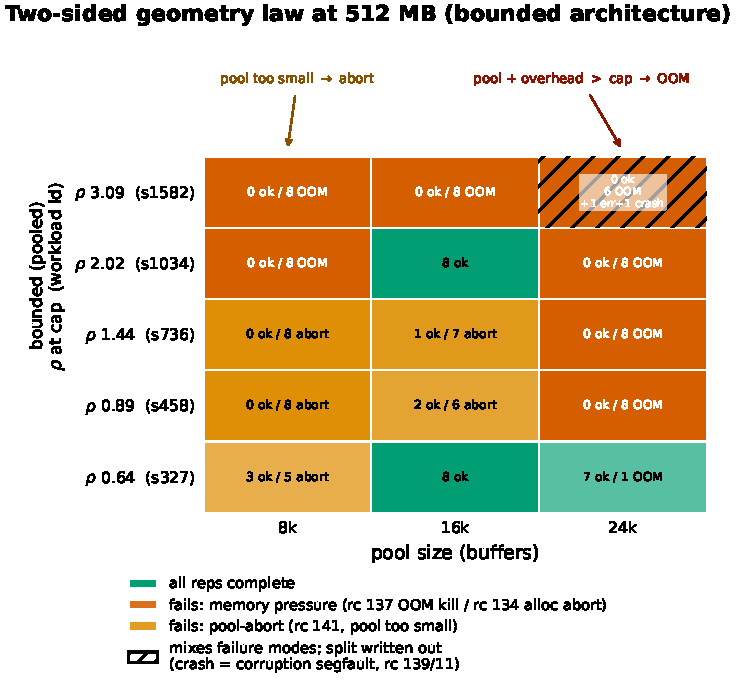
\includegraphics[width=0.85\textwidth]{img/fig_geometry_law_512.pdf}
\caption[The two-sided geometry law at 512\,MB]{The two-sided geometry law
at 512\,MB. Format: ``N ok / failure split'', e.g. ``0 ok / 8 abort''.\methodsnote}
\label{fig:geometry-law-512}
\end{figure}

At 1024\, MB, only the abort edge is reached because the tested pools never reach the OOM edge (Figure~\ref{fig:geometry-law-1024}).
Every plain failing cell is a pool abort, and a single OOM repetition sits inside s1582's mixed 16k cell.
Even at the largest pool tested (48k), the most pool-demanding workload, b1374, still aborts in full at 0 of 8.
The middle pool (32k) is transitional, with full completion at s458, half at s736 (4 of 8), and nothing above.

\begin{figure}[htbp]
\centering
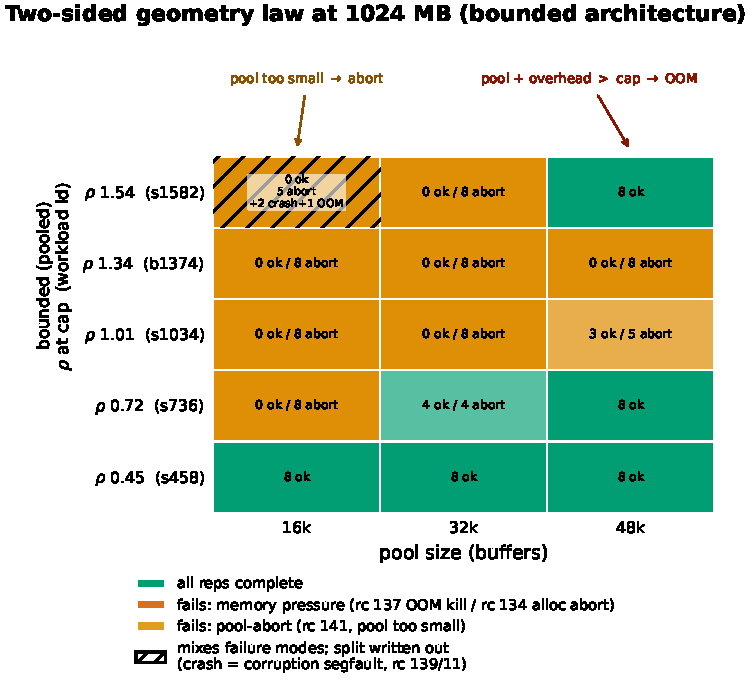
\includegraphics[width=0.85\textwidth]{img/fig_geometry_law_1024.pdf}
\caption[The two-sided geometry law at 1024\,MB]{The two-sided geometry
law at 1024\,MB. Same format as Figure~\ref{fig:geometry-law-512}.}
\label{fig:geometry-law-1024}
\end{figure}

At 2048\, MB, the abort edge determines the outcome for the heavier workloads tested, s1034 to b2078 against s327 to s1582 at 512\, MB (Figure~\ref{fig:geometry-law-2048}).
Only the largest pool (96k) or the lightest workload at 64k completes, and every plain-failing cell is a pool abort.
The OOM edge is never reached at this cap; a single OOM repetition sits inside s1582's mixed 16k cell, and the tested pool sizes fall short of the abort-to-OOM transition rather than crossing it.

\begin{figure}[htbp]
\centering
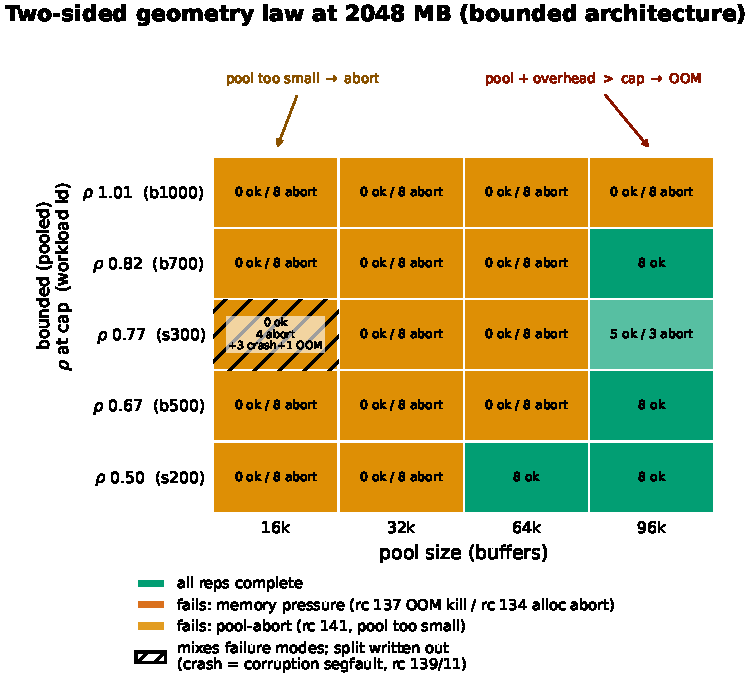
\includegraphics[width=0.85\textwidth]{img/fig_geometry_law_2048.pdf}
\caption[The two-sided geometry law at 2048\,MB]{The two-sided geometry
law at 2048\,MB. Same format as Figure~\ref{fig:geometry-law-512}.}
\label{fig:geometry-law-2048}
\end{figure}

% [7.6t]
The fast-ingest valley of Section~\ref{sec:rq1-race} recurs at every cap and pool; the pattern, completing runs ingesting below roughly 2.5 million tuples per second and failing runs whose demand exceeds roughly 2.7 million, appears 9 times across three caps and both allocation types.

% [7.6u]
The crash cluster is root-caused with sanitizer instrumentation.
Both custom allocators are invisible to \ac{ASAN}, so the pages were poisoned manually.
The cause is the per-worker slice cache, an engine default.
The cache passes raw map pointers to compiled code, and these accesses bypass the spill checks.
A stale cached pointer races a legitimate restore into the same map.
The diagnosis is tested in both directions and holds: with the cache on, 3 of 3 runs crash, and with the cache off, 4 of 4 complete cleanly.

% [7.6v]
Disabling the cache is no mitigation, for a structural reason.
With the cache off, every late write pins its slice until emission.
With jitter equal to the retention lag, the entire band is pinned, and no slice can spill; 0 of 8 complete at every cell, including cells that completed before, with zero slices spilled.
The two defects mask each other.
The headline data is unaffected, because the corruption manifests only in cells that fail regardless.

% [7.6v-bis — separate the corruption crash from a benign pressure abort]
The crash cluster must be separated from a second, benign process death.
Under a memory cap, the allocator can fail, aborting the process.
This abort has the same memory signature as an OOM kill; the run ends early, with memory at the cap, before completion.
It is therefore counted with the pressure failures rather than as corruption.
The corruption is a segmentation fault, root-caused above, and is counted separately.

The distinction matters for the marginal cells, those whose repetitions split between completion and failure.
A few pressure aborts fall in such cells, whereas every segmentation fault falls in a cell that never completes.
Counting a pressure abort as corruption would therefore place corruption inside partially completing cells; counting only the segmentation fault as corruption confines the crash cluster to cells that fail in every repetition.

% [7.6w]
The architectural conclusion is general.
Unmediated pointers into evictable state require an invalidation protocol.
Flink's backend mediates every state access; NebulaStream's slice cache does not.
The precise upstream fix is an epoch-stamped cache entry that is invalidated on spill and adds one comparison per cache hit.

\FloatBarrier
\subsection{The Growth Signal and Page Release in Operation\label{sec:growth-release-results}}

% [7.6x-intro] Subsection opening: the two remaining mechanisms in operation.
This subsection puts the two remaining mechanisms of Chapter~\ref{cha:solution} into operation: the growth signal, which turns out to be blinded by the same slice cache that causes the crash cluster, and page release, which reduces the resident floor but cannot reclaim a live slice.

% [7.6x]
The slice cache that causes the crash cluster also hides state growth from the growth signal.
The growth signal in Section~\ref{sec:growth-release} is designed to detect when a single slice exceeds a memory threshold, and its check runs inside the slice store.
Compiled query code reads and writes map state through the cache and never passes through the store, so the check never runs.
Placed inside the store, the signal records zero threshold crossings on a high-churn workload; placed on the per-record lookup path, which the cache cannot bypass, it records eight hundred.
The cache defect therefore has two consequences with a single root cause: restore-path corruption and undetected state growth.

% [7.6y]
With the signal restored, the remaining question is whether a single growing slice can break a run that the creation-time check would pass.
On a high-cardinality workload, one window's slice ranges from 127 to 157\,MB and crosses the hard threshold midway through the window, while the matched low-cardinality workload keeps every slice to 4\,MB.
The existing check runs only when a slice is created at a window boundary, so it never observes this growth; the growth signal does.

% [7.6z]
Evicting the growing slice when the signal fires holds it below the threshold and keeps the pool from filling, but converts no failing run.
The failure changes form instead of disappearing: either to an OOM kill, where resident memory is the limit, or to an allocation stall caused by the synchronous eviction itself, which blocks the ingesting thread.
A softer variant that only wakes the background spiller performs worse, because it removes the throttling the synchronous eviction provided, and the pool fills at full ingest speed.
The signal is necessary to observe intra-slice growth and insufficient to survive it; the binding limits remain the un-spillable hot slice and the minimum resident memory.

% [7.6aa]
Page release addresses the minimum resident memory.
On a draining workload, it cuts steady anonymous memory by 55 percent and peak by 38 percent, at a 6-to-8 percent throughput cost, completing every repetition.
Its effect is specific: on the single-hot-slice workload, it reclaims the cold band but cannot reclaim the live, growing slice, and that run still fails.
This result also clarifies the 14--22\% anonymous-memory advantage of pooling reported at the start of this section.
Recycling bounds the pool to what is concurrently live, and reuses freed buffers instead of growing the pool.
Page release returns freed pages to the operating system, so anonymous memory falls back to its working set instead of remaining at its peak.

% [7.6-answer] --- answer to RQ3
In response to RQ3, beyond the cap, memory follows the two-sided feasibility law: the pool must hold the hot band, or the run aborts; the pool plus its overhead plus the base footprint must stay under the cap, or the run is OOM-killed; and once the pool is sized right, completion depends on the ingest-drain race.
The remaining failures are therefore of three kinds: OOM kills where the footprint exceeds the cap, pool-exhaustion aborts where the pool is too small for the hot band, and a rare restore-path crash confined to cells already failing for a memory reason (Table~\ref{tab:outcomes}).
The pooled configuration keeps the footprint within this corridor by recycling pages through the pool.
The next section measures what this completion costs.

\section{Cost (RQ2)\label{sec:rq2}}

RQ2 asks what the backend costs are in terms of throughput and tail latency, and what spilling and restoring state cost on their own.
At a matched buffer size, the answer is a throughput cost of 11 to 16 percent, a 99th-percentile latency of 1.1 to 1.6 times that of the in-memory engine, and a resident footprint up to 33 percent smaller under the pooled configuration.
All headline comparisons use a matched \ac{IO} buffer size, about 8{,}000 bytes in every variant including the in-memory reference, so that each contrast measures the allocation choice rather than the buffer size; the buffer-size finding below justifies the choice.

% [7.3.1] + [7.3.2] --- throughput cost
Throughput is the first cost (Figure~\ref{fig:cost}(a)).
At a matched buffer size, \ac{OOC} processing costs 11--16\% of throughput when both variants complete, under either allocation type; the penalty grows with state size and shrinks with memory headroom.

% [7.3.4] + [7.3.3] + [7.3.7] --- tail-latency cost, confound separated
Tail latency is the second cost (Figure~\ref{fig:cost}(b)), and a naive comparison overstates it.
Comparisons at unmatched buffer sizes (the default-configuration row of Table~\ref{tab:cost}) show a 2--5$\times$ gap; per-task latency scales with buffer size across all variants, including the in-memory engine.
With the buffer size matched, the \ac{OOC} 99th percentile is 1.1 to 1.6 times the in-memory engine.
The remaining gap comes from the spill-restore round trip, and it appears in the tail.

Under unbounded allocation, tail latency grows into the millisecond range at ten-million-entry working sets; matching the buffer size reduces it, so that at the heaviest workload the 99th-percentile latency falls from 2509 to 899 microseconds while throughput rises by 36\%.
Spill and restore latencies are distributions rather than single numbers; their effect appears in the latency tail rather than in mean throughput, which is why the tables report both quantities.

% [7.3.5] --- buffer size as an engine-wide finding
Controlling for the buffer size produces a finding of its own.
The buffer size is an engine-wide performance factor, independent of \ac{OOC} processing; the same per-task latency scaling noted above also appears in throughput.
Increasing the default 4096-byte buffers to about 8{,}000 bytes increases throughput across all tested cells, and the in-memory engine alone gains up to 13\%.

% [7.3.6]
The pooled configuration's footprint advantage (Section~\ref{sec:rq3}) is confirmed at matched buffer size (Figure~\ref{fig:cost}(c)).
At the cell 2048/s1034, it uses 33\% less anonymous memory than the in-memory engine (924 versus 1388\, MB) and 27\% less than heap-allocated \ac{OOC}.
This 33\% is the widest among several footprint margins, rather than a single global figure; the narrower margins are those of Section~\ref{sec:rq3}, and the advantage grows as the pool shrinks.

\begin{figure}[htbp]
\centering
\widefig[0.95]{img/fig_cost.pdf}
\caption[The cost of out-of-core processing]{The cost of \ac{OOC} processing
at matched I/O buffer size ($\sim$8\,K buffers in every variant, same pool per
coordinate; means over completing repetitions), in three panels: (a) throughput,
(b) tail latency, (c) resident footprint, each relative to the in-memory
reference. In panel (a), the heap $-28\%$ at 512/s327 is excluded from the band;
its runs last only 2.5--4\,s, so the fixed startup phase dominates the measured
rate (Section~\ref{sec:rq4}).\methodsnote}
\label{fig:cost}
\end{figure}

% [7.3.8]
The cost depends on the configuration point, so Table~\ref{tab:cost} reports it as
bands across comparisons rather than a single figure.

\begin{table}[ht]
\centering
\small
\begin{tabular}{|>{\raggedright\arraybackslash}p{4.4cm}|>{\raggedright\arraybackslash}p{2.9cm}|>{\raggedright\arraybackslash}p{3.0cm}|>{\raggedright\arraybackslash}p{2.3cm}|}
\hline
\textbf{Comparison} & \textbf{Throughput} & \textbf{p99} & \textbf{Coverage} \\
\hline
Matched buffer size ($\sim$8\,K all variants) & $-11$ to $-16\%$ & 1.1--1.6$\times$ & 3 coordinates \\
\hline
Default configuration (own 4096 baselines) & $-3$ to $-22\%$ & $\mu$s $\to$ ms at $10^7$ keys & 6 coordinates \\
\hline
Bounded vs in-memory, anonymous-memory footprint & $-33\%$ (924 vs 1388\,MB) & $\approx$1.17$\times$ & 2048/s1034 \\
\hline
Nexmark transfer (in-order, supporting) & $-50$ to $-63\%$ & 1.1--1.2$\times$ & Nexmark C@1024 \\
\hline
\end{tabular}
\caption[Cost bands per comparison class]{Cost bands per comparison class. The Nexmark row compares against the
uncapped reference, because the capped engine fails this cell (0 of 8) and has
no baseline of its own.}
\label{tab:cost}
\end{table}

% [7.2.10]
The Nexmark transfer of Section~\ref{sec:nexmark} has a measurable cost, summarized in the last row of Table~\ref{tab:cost}.
In-order streams incur the full spill-and-restore round trip; on the synthetic grid this cost was not visible, because the out-of-order jitter kept the hot slices from spilling.
With the pre-committed cap-derived threshold, fitting workloads overspill and lose 42--61\% throughput for no benefit.
The completing beyond-memory cell loses 50--63\% against the unlimited reference.

The two configurations differ in the cost of their spilling.
On the repetitions they complete, the heap configuration is cheaper at six of the seven cells where both produce a measurement, by 2 to 12 percentage points, because it does not carry the pool bookkeeping, the queue pacing, and the paced restore of the bounded configuration; the bounded configuration is cheaper only at q3 scenario B under 1024\, MB.
The mechanisms that make the bounded configuration slower, the pool bookkeeping, the queue pacing, and the paced restore, are the same mechanisms that hold its memory under the cap at the beyond-memory point.
At that point, the heap configuration's lower cost is partly due to survivor bias, because it is measured only over the 6 and 3 heap repetitions that finished, compared with the bounded configuration's 8 and 7.
A state-aware spill threshold would remove overspilling; it is documented as future work and was deliberately not tuned on the evaluation workloads.
At the beyond-memory point, the backend retains roughly half the throughput of an engine with unlimited memory while spilling to a consumer SD card; on the same workload, the capped in-memory engine cannot finish at all.
Figure~\ref{fig:nexmark-cost} quantifies the cost; every \ac{OOC} point runs below the uncapped reference, with the lowest values in the fitting scenarios that over-spill under the fixed threshold.

\begin{figure}[htbp]
\centering
\widefig{img/fig_nexmark_cost.pdf}
\caption[Nexmark throughput cost]{Nexmark throughput cost: median throughput of
each \ac{OOC} configuration (bounded B2, heap U8) relative to the uncapped reference
for the same scenario, per query. In-order streams incur the full spill-and-restore
round trip, and the fixed cap-derived spill threshold over-spills the fitting
scenarios for no benefit; the completing beyond-memory cell (C at 1024\,MB) loses
50--63\% against the unlimited reference.\nexmarknote}
\label{fig:nexmark-cost}
\end{figure}

% [7.3.9] --- answer to RQ2
In answer to RQ2, at matched buffer size, the backend costs 11--16\% throughput where both allocation types complete, at a 99th-percentile task latency 1.1 to 1.6 times the in-memory engine.
Spilling and restoring state cost little in mean throughput; their cost appears in the latency tail, where the round trip raises the unbounded default into milliseconds at ten-million-entry sets.
An SD card is orders of magnitude slower than DRAM, yet the measured cost is 11--16\%; Section~\ref{sec:eval-summary} explains this gap from the mechanisms that the next two sections measure.

\section{Processor and Disk Utilization (RQ4)\label{sec:rq4}}

RQ4 asks how processor utilization and disk traffic evolve as the working set grows past the memory budget.
The answer is that utilization falls from near-full to disk-bound once spilling reaches the device, and that two separate mechanisms produce the idle time: disk waits and pool allocation stalls.

% [7.4.1] --- measurement basis and the in-memory baseline
All utilization figures here are the mean over the whole run.
The entire run includes the one-off query compilation phase at startup, which is single-threaded and takes a fixed amount of time regardless of the workload.
On short in-memory runs (two to fifteen seconds), the fixed cost lowers mean utilization, so the in-memory engine runs at 84--97\%, lowest on the shortest cells; on long runs, it amortizes away, and utilization reaches about 99.6\%.
The in-memory engine has zero disk traffic.

% [7.4.1b] --- disk reads split at the memory boundary
Below the memory boundary, restores are served from the operating system's page cache, and device reads are at or near zero in 22 of the 24 spilling cells.
Above the boundary, the spilled state exceeds the page cache, and every spilling cell reads from the device (57 to 511\, MB per run); the cells that complete there run at 62--87\% with write-dominated traffic.

% [7.4.1c] --- two mechanisms lower utilization
The lower figures in Figure~\ref{fig:cpu-io}(a) are idle time rather than the compilation cost, and two mechanisms produce them.
The first is disk wait.
The bottom of the range is the throttled regime, in which demand exceeds the pool but the cap throttles ingest instead of the run deadlocking (regime two of the three-regime feasibility law, Section~\ref{sec:rq3}); there the workload is disk-bound at 62\% utilization with heavy traffic in both directions (278\, MB read, 525\, MB written).
The second is pool-allocation stalling in the bounded configuration.
The largest probed pool at each cap produces the lowest utilization of its panel, 31\% for s327 at 512\, MB (24k buffers), 64\% for s458 at 1024\, MB (48k), and 54\% for b1676 at 2048\, MB (96k), with near-zero device reads and runtimes up to three times longer than at smaller pools on the same workload.
The cause is the up-front pool reservation, which reduces the memory available for ingest (the mechanism of Section~\ref{sec:rq1-windows}).

% [7.4.2]
Disk read and write volumes scale with the spilled state volume (Figure~\ref{fig:cpu-io}(b)).
The SD card's write bandwidth bounds the drain rate in the race from Section~\ref{sec:rq1}.

% [7.4.3] --- transition; the section's opening paragraph carries the answer.
The next section turns from the traffic itself to how efficiently the spilled and resident bytes are used.

\begin{figure}[htbp]
\centering
\widefig{img/fig_cpu_io.pdf}
\caption[Average processor and disk behavior across state pressure]{Average
processor and disk behavior across state pressure (completing cells of the grids;
cgroup CPU and I/O accounting, medians per cell). (a) CPU utilization; the
plot itself annotates the one-off compilation-phase effect on short runs. (b)
Disk read/write volume for spilling cells.\methodsnote}
\label{fig:cpu-io}
\end{figure}

\section{Storage Efficiency (RQ5)\label{sec:rq5}}

% [7.5.0] Opening frame: how this section answers RQ5.
RQ5 asks how efficiently storage is used along the two dimensions it names: the composition of the memory footprint and the write amplification of spilling.
The answer is a write amplification of 1.0 to 1.8 at device level and a footprint of 51\% headers, 34\% payload, and 14\% bucket directory, of which roughly 17 to 20 percent is structurally recoverable but left unimplemented.

% [7.5.1] Footprint composition.
Entry headers dominate the state footprint.
The per-map gauge, decomposing the state at 26 million entries, attributes 51\% to headers, 34\% to payload, 14\% to the bucket directory, and below 1\% to page slack (Figure~\ref{fig:composition}(a)).
The bucket directory is the map's control block that indexes its entries.
It spills with the entries and is reconstructed byte-for-byte on restore because the serializer writes the exact map layout, including the directory, so a restore is a plain byte copy.

% [7.5.2] Reducible overhead: the unused header pointer.
Two parts of that footprint are structural overhead a refactor could remove, and both are quantified but left unimplemented.
The first is in the header.
Eight bytes of every 24-byte header is a pointer for virtual dispatch that is never used, one third of each header.
Removing it would recover about 20\% of an entry's 40-byte header-plus-payload record, roughly 17\% of total state once the bucket directory is included (the $\approx$20\% marked on the bar of Figure~\ref{fig:composition}(a)).
The removal requires an entry-inheritance refactor; it is documented and not implemented.

% [7.5.3] Reducible overhead: the oversized bucket directory.
The second is the bucket directory, which is larger than the workload needs.
A one-line fix changed the bucket count at only one of the three sites that assign it, the slice-creation path, and left the per-worker build and the unspill/merge path unchanged, so two-thirds of the maps kept their original directory size.
Completion was unaffected.

% [7.5.4] Write amplification.
Spilling writes 1.0 to 1.8 device bytes per byte of spill-directory volume with lz4 compression, including compaction; this is the write amplification measured at device level.
It is a device-level proxy rather than RocksDB's internal counter, which was not captured uniformly.

% [7.5.4b] On-disk spill volume (panel b).
The on-disk spill volume depends solely on the workload and its compression.
Where both allocation types complete the same cell, their spill directories are the same size, so the heap and bounded markers coincide in Figure~\ref{fig:composition}(b).
Heap contributes fewer points there because the bounded campaign probed more pool and cap coordinates, and heap fails the high-pressure cells due to the completion race in Section~\ref{sec:rq1-race}.

% [7.5.5]
A pool-sizing rule combines the two bounds of the geometry law (Section~\ref{sec:rq1-geometry}) with a designed safety margin.
The rule is to size the pool so that it holds the hot band and, together with its unpooled overhead and the base footprint, stays below 90\% of the cap.
The base footprint is the resident memory outside the pool and the unpooled directories, the engine and runtime baseline, plus the working set that the gauges do not attribute, and the RocksDB set included (decomposed in Figure~\ref{fig:rb32-compartments}, \hyperref[app:rb32]{Appendix~E.6}).
The data does not itemize the soft budget, the emission pipeline, or the I/O path on their own, and the 90\% margin is chosen to leave headroom for them rather than measured from them.

% [7.5.6] Answer to RQ5.
In answer to RQ5, the shipped layout spills at a device-level write amplification of 1.0 to 1.8 and carries no measured waste beyond page slack; the unrealized headroom of roughly 17 to 20 percent, the unused header pointer and the oversized bucket directory, is documented rather than implemented.
The next section collects the verdicts for all research questions.

\begin{figure}[htbp]
\centering
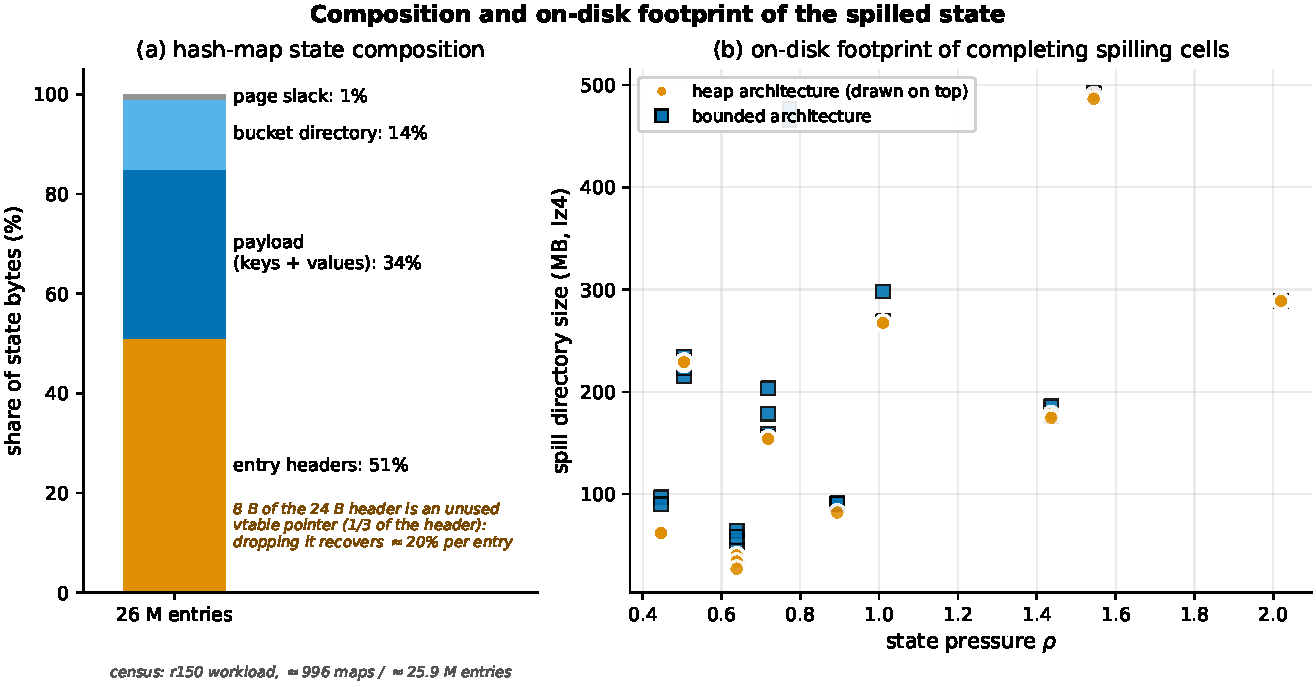
\includegraphics[width=0.8\textwidth]{img/fig_composition.pdf}
\caption[Composition of the state footprint]{Composition of the state
footprint. (a) Stacked decomposition of hash-map state bytes from the per-map
gauge census (s736 workload, $\approx$996 destructed maps, $\approx$25.9 million
entries) into entry headers, payload, bucket directory, and page slack; the
marked $\approx$20\% of each header-plus-payload record is the unused 8-byte
vtable pointer in each header. (b) On-disk spill-directory size (lz4) of
completing spilling cells against state pressure $\rho$, one marker per cell:
squares for the pooled configuration, circles for heap.\methodsnote}
\label{fig:composition}
\end{figure}

\section{Summary of Results\label{sec:eval-summary}}

% [7.7.1] Lead + verdict table; each verdict was developed in its section.
Every research question is answered, and Table~\ref{tab:verdicts} condenses the verdicts into a single row per question.
RQ0, the integration question, is answered by construction; the spillable slice store sits behind the unchanged store interface and ran through about 3{,}100 measured runs without changes to the query-compilation pipeline (Chapter~\ref{cha:solution}).

\begin{table}[ht]
\centering
\small
\begin{tabular}{|p{1.4cm}|p{5.2cm}|p{6.2cm}|}
\hline
\textbf{RQ} & \textbf{Verdict} & \textbf{Strongest single number} \\
\hline
RQ0 & Met by construction and operation & $\sim$3{,}100 runs executed through the unchanged store interface \\
\hline
RQ1 & Met inside a characterized window & 14/24 vs 0/18 at 512\,MB, $p = 4.1 \times 10^{-5}$, checksums match while spilling \\
\hline
RQ2 & Met & $-11$ to $-16\%$ throughput at matched buffer size; p99 1.1--1.6$\times$ \\
\hline
RQ3 & Met & attribution ladder 0/10 $\to$ 7/8; pooled vs.\ unpooled levers 12/16 vs 0/16, $p = 8.1 \times 10^{-6}$; deadlock shown in 118/138 stalls \\
\hline
RQ4 & Met & throttled regime at 62\% CPU, I/O-bound \\
\hline
RQ5 & Met with a stated proxy & headers 51\% of state; write amplification 1.0--1.8 (device level) \\
\hline
\end{tabular}
\caption[Verdict per research question]{Verdict per research question.}
\label{tab:verdicts}
\end{table}

% [7.7.2] Headline significance across the chapter, collected in one figure.
% Placed here so every row refers backward to a contrast already developed.
Figure~\ref{fig:pvalues} presents the chapter's headline completion contrasts in a single view, each a two-configuration comparison of completed versus attempted runs, with its Fisher's exact $p$-value.
The rows are, from top to bottom, the primary finding (Section~\ref{sec:rq1-headline}), the lever effect within pooling and the same levers without pooling (Section~\ref{sec:rq3}), and the allocation-type contrast (Section~\ref{sec:disambiguation}); each was developed in the section named, and here they stand side by side.
Every headline contrast has $p < 10^{-3}$.

% [7.7.3] Resolve the apparent tension between the primary-finding and allocation rows.
Two of these rows involve the heap configuration, and read side by side they appear to conflict; at the same workload and cap, the heap completes the primary-finding contrast yet fails the allocation-type contrast.
The two rows measure different things.
The primary-finding row sets the heap configuration against the capped in-memory engine, which cannot spill at all, so its axis is spilling versus its absence, and the heap completes out-of-core (14/24 versus 0/18).
The allocation-type row sets two configurations that both spill and holds the I/O buffer size fixed so that only the allocation type differs; its heap side is therefore the matched-buffer-size control of Section~\ref{sec:disambiguation} rather than the engine-default heap of the primary finding.
At s1034 and 512\, MB, the control's unbounded per-slice growth raises resident memory to 496 of 512\, MB, and it is OOM-killed 0 of 8.
The bounded pool holds the same working set at 390\, MB and completes 8 of 8.
The primary finding's default heap, with its smaller buffers, fits at 411\, MB and completes 8 of 8.
The heap configuration thus completes more than not-spilling and less than bounded-spilling at the tightest cell; the rows differ in baseline and configuration and do not contradict each other.

% [7.7.4] Interpreting the cost: a factor where the device gap suggests an order of magnitude.
DRAM and a consumer SD card differ by orders of magnitude in bandwidth and access latency, so a backend that moves window state between them could be expected to lose an order-of-magnitude drop in throughput.
The measured loss is 11 to 16 percent where both allocation types complete, and 50 to 63 percent at the beyond-memory Nexmark point.

Four measured mechanisms close this gap.
First, the operator reduces before it stores; an aggregation keeps one accumulator per key, so most tuples update bytes already resident, and only the compacted state reaches the device, resulting in device-level write amplification of 1.0 to 1.8 (Section~\ref{sec:rq5}).
Second, the hot band remains resident because the Zipfian skew concentrates most updates on a few keys (Section~\ref{sec:setup}), and on the out-of-order grid, the hot slices never spill at all (Section~\ref{sec:nexmark}).
Third, restores below the memory boundary are served from the page cache, with near-zero device reads in 22 of 24 spilling cells (Section~\ref{sec:rq4}).
Fourth, the spiller writes in the background, so the device's latency overlaps with computation and only its bandwidth limits the run, which is the race of Section~\ref{sec:rq1-race}.
How much each mechanism contributes individually was not isolated; the list states the measured effects without assigning each mechanism its share.

The moderate cost therefore holds only while reduction, skew, and caching keep the byte stream to the device below the drain bandwidth.
Where a condition falls away, the cost grows, as the in-order Nexmark stream shows, and a slower storage device narrows the margin in proportion (Section~\ref{sec:threats}).

\begin{figure}[htbp]
\centering
\widefig{img/fig_pvalues.pdf}
\caption[Headline completion contrasts and their significance]{Headline
completion contrasts and their significance, one row per contrast (labeled on
the plot, with its underlying completion counts annotated beside each point).
(a) Effect size: the completion-difference point estimate with its 95\%
confidence interval (Newcombe's method \cite{newcombe1998}, built from Wilson score intervals on
each configuration's completion proportion). (b) Significance: Fisher's exact $p$-value on a log
scale, with a dashed reference at $p = 0.05$. Every contrast lies below that line
by orders of magnitude; each row is developed in the section named in the
text.\methodsnote}
\label{fig:pvalues}
\end{figure}

\section{Threats to Validity\label{sec:threats}}

% [8.1]
Nine limits bound these results.
First, the hardware setup emulates an edge device's resource envelope and is not one.
All experiments were run on a single desktop host with a single SD card, under a cgroup memory cap, a pinned two-core budget, and SD-card spill storage (Section~\ref{sec:reproducibility}); this reproduces the resource limits of a constrained edge node rather than its hardware.
A real device with a different processor, memory subsystem, or flash controller may behave differently, so the absolute figures here, throughput, latency, and the exact position of the failure boundaries, describe the backend's behavior under a controlled budget rather than predicting any specific device.
The direction of the contrasts between configurations is expected to transfer, and the research questions ask about this direction; the absolute magnitudes are not claimed to transfer.

Second, the primary workloads are synthetic; this is in scope by design, and the Nexmark-style stream provides the transfer test.
Third, between measurement sessions throughput drifts 4--17\%, so all key contrasts are within-session.
Fourth, $\rho$ for the largest workloads is derived from in-memory footprints at 2048\, MB.
Fifth, checksum coverage is partial, with two workload points per allocation type.
Sixth, the allocation-type versus buffer-size confound existed in early comparisons; the dedicated disambiguation configuration resolved it (Section~\ref{sec:disambiguation}).
Seventh, roughly a dozen corrupted cells are confined to already-failing regions and are root-caused (Section~\ref{sec:geometry-valley}).

Eighth, the evaluation covers a fixed subset of the configuration space; every parameter except the memory cap, the workload state, the pool size, and the allocation type is held at the single value of Section~\ref{sec:setup}, and the RocksDB backend is pinned at 16/8 (Section~\ref{sec:rocksdb-config}).
The findings are conditional on these choices, and other window lengths, lateness bounds, page sizes, compression codecs, or backend sizes may shift the reported boundaries.
The evaluation demonstrates that the backend completes state larger than memory by spilling to and restoring from storage under this tested subset; behavior elsewhere in the design space is not established.
Ninth, each cell carries only 8 to 10 repetitions, so per-cell completion fractions carry wide 95\% confidence intervals (8 of 8 spans 68 to 100 percent) and must be read as estimates rather than fixed values; the chapter's claims rest on the headline contrasts, which have $p < 10^{-3}$, rather than on individual cells.

% [8.2]
The pinning rule in Section~\ref{sec:setup} stems from a single incident.
An early sweep produced a fake optimum because one binary default, the page size, differed from the baseline.

The next chapter relates these findings to existing systems and studies.

    \chapter{Related Work\label{cha:related}}
% Drafted per POINT-SEQUENCE.md Ch.6 (points 3.1–3.7).

This chapter situates the thesis alongside existing systems and studies.
It covers the reference integration of RocksDB in stream processing, work on larger-than-memory window state, the tuning literature, and the methodology this thesis follows.

\section{RocksDB as a State Backend in Stream Processing\label{sec:rel-flink}}

% [3.1]
Apache Flink is a widely used stream processing system.
Flink ships RocksDB as its production out-of-core state backend~\cite{flink2021}.
This integration is the reference point for state that exceeds memory in stream processing.

% [3.2]
Flink's runtime differs from NebulaStream's in two ways that block direct transfer of its results.
Flink organizes its state access around checkpoints, which are periodic snapshots for fault tolerance.
Its data exchange is pull-based at the boundaries that Marcu and Bouvry analyze~\cite{marcu2022}.
NebulaStream pushes data through pipelines and shares one global buffer pool across all operators (Section~\ref{sec:bg-nes}).
Results from Flink therefore do not transfer directly to NebulaStream.

% [3.5]
A separate line of work studies RocksDB's parameters.
Jin et al.\ show that large-scale parameter tuning improves performance but leaves substantial write amplification even after optimization~\cite{jin2022}.
Ad\~ao et al.\ co-design the storage hierarchy below the \ac{KV} store and show that data placement across devices, not tuning alone, governs its I/O performance~\cite{adao2025}.
Wei et al.\ analyze the write amplification of RocksDB's compaction policies and show that even the best policy retains substantial write amplification~\cite{wei2025}.
Together, these studies show that configuration mitigates but does not remove the write and I/O costs.
This thesis therefore fixes a single research-informed configuration rather than searching over configurations (Section~\ref{sec:bg-rocksdb}).

\section{Larger-than-Memory Window State\label{sec:rel-windows}}

% [3.3]
WindFlow demonstrates larger-than-memory windowed processing in a single-node engine~\cite{frassinelli2025}.
Larger-than-memory window state is therefore addressed beyond Flink.

% [3.4]
AION keeps window state across memory and persistent storage so that late
events can still update windows that have already closed~\cite{esteves2020}.
It bounds storage growth with proactive caching and predictive cleanup.
Like this thesis, it pushes window state out of memory onto a storage device
(Section~\ref{sec:bg-windows}), though for late-event handling rather than a hard memory cap.

Neither WindFlow nor AION evaluates a push-based engine with one shared global buffer pool under hard memory caps.

\section{Evaluation Methodology\label{sec:rel-method}}

% [3.6]
Fragkoulis et al.\ survey the evolution of stream processing systems, including their state management~\cite{fragkoulis2024}.
The thesis pre-registers its hypotheses and reports negative results in full.
Chapter~\ref{cha:evaluation} applies this discipline throughout.

\section{Positioning\label{sec:rel-positioning}}

% [3.7]
To the best of the author's knowledge, no published work evaluates an out-of-core window-state backend within a push-based engine with a single shared global buffer pool under hard memory caps.
This thesis provides this evaluation.
Its contribution is evaluation-first; the backend exists to enable measurement.

The next chapter summarizes what the evaluation establishes and what remains open.

    \chapter{Conclusion\label{cha:conclusion}}
% Drafted per POINT-SEQUENCE.md Ch.7 (WP 9.1–9.3 + 8.3–8.4).

This chapter concludes the thesis. It summarizes the contributions, states their limitations, and closes with practical guidance, lessons learned, and future work.

\section{Summary\label{sec:summary}}

This thesis asks whether NebulaStream can process window state larger than memory on edge-class devices.
Within the evaluated scope, the answer is yes.
Under hard memory caps, the spillable backend completes workloads whose state exceeds the memory budget and which the unmodified engine cannot finish, with matching output checksums and at a bounded throughput cost.
The thesis builds this backend as a spillable slice store with RocksDB as the storage engine, evaluates it under hard memory caps across roughly 3{,}100 measured runs, and investigates every failure until its cause is known.

% [9.1 — one conclusion per contribution]
The seven contributions hold as follows.
C1: the backend integrates behind the unchanged store interface and operates across the full evaluation without changes to the compilation pipeline.
C2: the harness reproduces every result from a single binary, with pre-registered hypotheses and six memory probes; the evaluation data and analysis documents are versioned alongside the code.
C3: the backend prevents OOM failures inside characterized operating windows per memory budget (Table~\ref{tab:windows}), and completion depends on the race between ingest and drain rather than on a state-size threshold.
C4: a single engine default kept all window state outside the buffer pool in every configuration.
The one-flag pooled configuration with pool-pressure levers reaches, at one measured cell (1024\,MB cap, 32k pool, s736), 98\% of the in-memory engine's throughput at 25\% less anonymous memory (517 versus 685\, MB, Section~\ref{sec:rq3}).
The same allocation distinction determines how to size the RocksDB backend (\hyperref[app:rb32]{Appendix~E.6}).

C5: the failures follow a three-regime feasibility law, and the residual failure is an allocation deadlock in which emitted state pins the buffer pool while the workers that would drain it are all blocked on allocation, as demonstrated by direct instrumentation (Figure~\ref{fig:gridlock}).
C6: all mechanisms ship configuration-gated in an open branch; with gates closed, the engine is byte-identical to the baseline.
C7: the growth signal makes intra-slice growth visible on the production path once the slice cache is bypassed, and the page-release extension cuts steady anonymous memory on draining workloads by 55\% below what pooling alone retains after a drain; neither resolves the residual deadlock, which remains bound by the un-spillable hot slice and the minimum resident memory.

% [negative IoT finding — advisor note 2]
The evaluation also yields one negative finding: once the storage device's write bandwidth is the bottleneck, no engine-side mechanism can remove that limit.
In the \ac{IoT}, the ingestion rate and the storage device are not fixed.
A deployment must assume that both vary widely across nodes.
The ingestion rate is set by the sensors and the network rather than by the engine.
The storage device is the SD card the node carries, and SD card write bandwidth varies by an order of magnitude across cards.

This matters because completion depends on the race between ingest and drain (C3).
The spiller can only drain state to disk as fast as the card accepts writes.
The SD card's write bandwidth therefore bounds the drain rate (Section~\ref{sec:rq4}).
When the card is slow, the storage-bandwidth ceiling drops, and the band of ingest rates the engine can sustain shrinks with it.
The moderate throughput cost reported for RQ2 depends on the same margin; it is a property of the tested card as much as of the backend, and the mechanisms that keep it moderate (Section~\ref{sec:eval-summary}) assume the device keeps up with the compacted spill stream.

The practical consequence is that once storage is the bottleneck, the I/O path sets the limit, as no engine mechanism can increase the storage device's write bandwidth.
The deployment must instead address the I/O path directly by choosing a faster device, reducing the number of bytes written per window, or throttling ingest to stay under the storage-bandwidth ceiling.
The three-regime law reaches the same conclusion from the other side (Section~\ref{sec:rq3}); in the disk-bound regime, the run survives only by holding ingest below the rate the device can drain.

\section{Limitations and Generalizability\label{sec:generalizability}}

% [8.3] Four kinds of limits: parameter-space scope, statistical certainty, system specificity, the rho metric.
Four kinds of limits bound these conclusions, and each conclusion above should be read in light of them.

The first limit is scope.
The evaluation covers a deliberately fixed subset of the design space; only the memory cap, the workload state, the pool size, and the allocation type were varied, while the window length, lateness bound, page size, compression, RocksDB configuration, partition count, core count, host, storage device, and query shape were each held at a single value (Section~\ref{sec:threats}).
This targeting made the memory question answerable, but the conclusions therefore describe the tested subset rather than the solution space; other parameter choices may shift the operating windows, the cost bands, and the failure boundaries.
The evaluation demonstrates the core capability independently of those choices; the backend processes state larger than memory by spilling to and restoring from storage, with correct output.
The exact boundary positions reported in Chapter~\ref{cha:evaluation} depend on the configuration and should not be carried over to other setups as fixed values.

The second limit is statistical.
Each cell carries only 8 to 10 repetitions, so per-cell completion fractions carry wide confidence intervals and are estimates rather than fixed values.
The claims this thesis relies on are therefore the headline contrasts, which have $p < 10^{-3}$; individual cell fractions, and the between-session absolute magnitudes affected by the 4--17\% throughput drift, carry correspondingly less certainty.

The third limit is system specificity.
The effectiveness claim holds inside the characterized windows rather than universally.
The specific thresholds, the pooling boundary, and the slice cache are NebulaStream-specific.
The three-regime feasibility law and the deadlock pattern are stated in terms of one fixed shared buffer pool.
Any engine with this property is plausibly expected to exhibit the same regimes; verifying this is future work.

The fourth limit is the $\rho$ metric itself.
$\rho$ is defined as the uncapped workload's steady-state anonymous footprint divided by the cap (Section~\ref{sec:bg-metrics}) and is used throughout as if it were a fixed property of the workload, independent of the cap against which it is tested.
It is not fully independent.
At the one cell checked closely, s1034 at 1024\, MB ($\rho \approx 1.01$, Figure~\ref{fig:effectiveness}), the uncapped reference run is measurably a different execution than the same workload run under the real cap, about 14\% slower and correspondingly heavier in peak anonymous memory, with no overlap across repetitions.
The same pattern holds in the two other workloads checked.
s736 runs 16\% slower uncapped than at its 1024\, MB cap (2.90 versus 3.43\, M tuples/s, no overlap across repetitions), and s1582 runs 10\% slower uncapped than at its 2048\, MB cap (2.48 versus 2.77\, M tuples/s, likewise no overlap); lower throughput and higher peak memory move together in both, well away from the boundary cell that motivated the check.

The likely mechanism is memory-allocator behavior.
An allocator under no pressure to reuse freed memory allows a process's live data to spread across more pages, increasing memory usage and reducing locality, whereas a hard cap forces tighter reuse.
This account fits the data but is not independently confirmed; no allocator- or engine-level instrumentation was collected to isolate the exact mechanism, so it stands as the best-supported explanation rather than a demonstrated one.
The consequence is that $\rho$, computed from the uncapped reference, mildly overstates true pressure at a given cap.
The qualitative boundary this thesis reports (workloads clearly below $\rho = 1$ complete, workloads clearly above fail) is unaffected, but near that boundary $\rho$ should be read as approximate rather than exact, because the state actually resident differs between the uncapped and the capped execution modes the metric compares.

\section{Practical Guidance\label{sec:guidance}}

% [8.4]
For an edge deployment of NebulaStream, the evaluation supports one recipe, within the scope stated above.
Enable page pooling by raising the operator buffer size to the page size.
Size the pool according to the rule in Section~\ref{sec:rq5} so that it holds the hot band and, together with its overhead and the base footprint, remains below 90\% of the cap.
Derive the soft threshold from the memory cap rather than from the pool (Section~\ref{sec:rq3}).
Enable the reserve lever at 15\% and paced restore.
Leave allocation backpressure off.

\section{Lessons Learned\label{sec:lessons}}

Five working rules emerged from the investigation and are recorded here for successors.
Pin every configuration knob explicitly; a single differing binary default produced a false optimum.
Pre-register every hypothesis; refuted explanations are as informative as confirmed ones.
Report negative results in full; three of the six design mechanisms converted nothing, and stating this plainly is part of the contribution.
Verify the allocation assumption behind every experiment; the levers acted on a pool without window state for an entire campaign.
Validate component benchmarks at the system level; the storage backend's component-level byte savings did not hold under the memory cap.

\section{Future Work\label{sec:future}}

% [9.2 — in order of precision]
Figure~\ref{fig:final-status} shows the final status of the subsystem and pins
each improvement below to the component it would modify.
Future work is listed in order of how precisely it is specified.

% Final status of the out-of-core subsystem + future-improvement overlay.
% Use as: % Final status of the out-of-core subsystem + future-improvement overlay.
% Use as: \input{figures/final_status_uml}   (preamble needs tikz, see Template.tex)
%
% LAYOUT — strict raster so no element can overlap another:
%   Column centres : x = 0, 7.4, 14.8   (pitch 7.4 cm, boxes 5.2 cm wide -> 2.2 cm gaps)
%   Row centres    : y = 0, -3, -6, -9, -12, -15   (pitch 3 cm, boxes <= 2.6 cm tall)
%   Future badges  : dashed red circles pinned at box corners, poking into the
%                    column gaps only; the F-numbers resolve in the band below.
%   Edge labels    : white badges (style "lbl"), placed on vertical runs or on
%                    same-row horizontal runs only — no diagonal label can graze a box.

\begin{figure}[H]
\centering
\resizebox{\textwidth}{!}{%
\begin{tikzpicture}[
  font=\sffamily\small,
  every node/.style={align=center},
  box/.style ={rectangle, draw, thick, minimum width=5.2cm, minimum height=1.5cm,
               inner sep=4pt, rounded corners=1pt},
  existing/.style ={box, fill=black!12},
  newcomp/.style  ={box, fill=blue!18},
  storage/.style  ={box, fill=orange!28, double, double distance=1pt},
  hook/.style     ={box, fill=yellow!55},
  flow/.style={-{Latex[length=2.4mm]}, thick},
  impl/.style={-{Triangle[open, length=3.2mm, width=3.2mm]}, thick},
  warn/.style={-{Latex[length=2.4mm]}, thick, dashed, red!60!black},
  lbl/.style={fill=white, draw=black!30, line width=0.2pt, rounded corners=1pt,
              inner sep=2pt, font=\sffamily\footnotesize\itshape, text=black!75},
  fbadge/.style={circle, draw=red!70!black, dashed, thick, text=red!70!black,
                 fill=white, font=\sffamily\bfseries\footnotesize, inner sep=1.6pt},
]

\def\cA{0} \def\cB{7.4} \def\cC{14.8}

% ================= COLUMN A : store path =================
\node[existing] (handler) at (\cA,0)
  {WindowBasedOperatorHandler\\\footnotesize\itshape triggers windows, drives emit};
\node[existing] (iface) at (\cA,-3)
  {WindowSlicesStoreInterface\\\footnotesize\itshape «interface», unchanged\\\footnotesize\itshape (requirement R4 met)};
\node[newcomp, minimum height=2.6cm] (store) at (\cA,-6.2)
  {\textbf{SpillableTimeBasedSliceStore}\\[1pt]
   \footnotesize soft / hard thresholds $\cdot$ spiller (100\,ms)\\
   \footnotesize levers 1a reserve $\cdot$ 1b rescue\\
   \footnotesize 1c paced restore $\cdot$ 1d dir.\ accounting};
\node[newcomp] (bp) at (\cA,-9.6)
  {Allocation backpressure\\\footnotesize\itshape + progress guard (converted\\\footnotesize\itshape nothing); ships as diagnostics};

% ================= COLUMN B : state path =================
\node[newcomp] (cfg) at (\cB,0)
  {SpillConfig «configuration»\\\footnotesize\itshape every mechanism gated; all gates\\\footnotesize\itshape closed $\Rightarrow$ byte-identical baseline};
\node[newcomp] (slice) at (\cB,-6.2)
  {\textbf{SpillableAggregationSlice}\\\footnotesize : HashMapSlice $\cdot$ resident flag\\\footnotesize spill() $\cdot$ unspill()\\\footnotesize\itshape hot $\cdot$ cold $\cdot$ spilled $\cdot$ restored $\cdot$ emitted};
\node[newcomp] (serializer) at (\cB,-9.6)
  {SliceSerializer\\\footnotesize\itshape page-exact layout;\\\footnotesize\itshape restore = plain byte copy};
\node[newcomp] (backend) at (\cB,-12.6)
  {SpillBackend «interface»\\\footnotesize put $\cdot$ get $\cdot$ erase};
\node[storage] (rocks) at (\cB,-15.4)
  {RocksDBSpillBackend\\\footnotesize\itshape lz4 $\cdot$ SD-card spill target};

% ================= COLUMN C : memory side =================
\node[existing] (bufmgr) at (\cC,0)
  {BufferManager\\\footnotesize + \textcolor{blue!50!black}{availability query $\cdot$ pressure}\\\footnotesize \textcolor{blue!50!black}{listeners $\cdot$ recycle counter}};
\node[hook] (chained) at (\cC,-3)
  {ChainedHashMap pooling boundary\\\footnotesize\itshape pooled iff page size $\leq$ buffer size;\\\footnotesize\itshape 8192-flag = pooled configuration};
\node[existing] (cache) at (\cC,-6.2)
  {Per-worker slice cache\\\footnotesize\itshape raw map pointers\\\footnotesize\itshape bypass the spill checks};
\node[newcomp] (gauges) at (\cC,-9.6)
  {Six memory gauges\\\footnotesize cgroup $\cdot$ pool $\cdot$ unpooled\\\footnotesize map $\cdot$ spill $\cdot$ backpressure};

% ================= EDGES =================
\draw[flow] (handler) -- node[lbl]{uses} (iface);
\draw[impl] (store) -- node[lbl]{implements} (iface);
\draw[flow] (store) -- node[lbl, pos=0.5]{manages} (slice);
\draw[flow] (slice) -- node[lbl, pos=0.74]{serialized by} (serializer);
\draw[flow] (serializer) -- node[lbl]{pages as key--value pairs} (backend);
\draw[impl] (rocks) -- node[lbl]{implements} (backend);
% config tunes the store: route through the A--B column gap (x = 3.7)
\draw[flow, rounded corners=6pt] (cfg.west) -| (3.7,-5.6) -- ($(store.east)+(0,0.6)$);
\node[lbl] at (3.7,-2.1) {tunes};
% buffer manager notifies the store (lever 1b): vertical run in the B--C gap
% (x = 11.1), horizontal run at y = -7.9 (clear of the slice row above and the
% serializer row below), then up into the store's south edge.
\draw[flow, rounded corners=6pt] (bufmgr.west) -| (11.1,-7.9) -| ($(store.south)+(0.9,0)$);
\node[lbl] at (11.1,-4.2) {pressure\\listeners\\(lever 1b)};
% slice cache races restores — same-row horizontal, dashed warning
\draw[warn] (cache.west) -- node[lbl, text=red!60!black]{races\\restores} (slice.east);
% buffer manager pages for the hash maps
\draw[flow] (bufmgr) -- node[lbl]{rents pages} (chained);

% ================= FUTURE-IMPROVEMENT BADGES =================
\node[fbadge] at ($(bufmgr.north east)+(-0.05,0.05)$)  {F1};
\node[fbadge] at ($(bufmgr.south east)+(-0.05,-0.05)$) {F2};
\node[fbadge] at ($(chained.north east)+(-0.05,0.05)$) {F3};
\node[fbadge] at ($(slice.north east)+(-0.05,0.05)$)   {F4};
\node[fbadge] at ($(cache.north east)+(-0.05,0.05)$)   {F5};
\node[fbadge] at ($(store.north east)+(-0.05,0.05)$)   {F6};

% ================= FUTURE-WORK BAND =================
\node[draw=red!70!black, dashed, thick, rounded corners, fill=red!4,
      text width=19.6cm, inner sep=8pt, align=left,
      font=\sffamily\footnotesize] (future) at (\cB,-18.6)
  {\textbf{\textcolor{red!70!black}{Potential further improvements (Section~\ref{sec:future}, in order of precision)}}\\[3pt]
   \textbf{F1} role-aware allocation, a drain-side reserve that build-path allocations cannot consume; merges the two allocation types' operating windows\\
   \textbf{F2} closed-loop ingest admission keyed to pool headroom; replaces accidental throttling by the cap with a deliberate mechanism\\
   \textbf{F3} entry-header refactor: remove the unused virtual-dispatch pointer ($-$20\,\% state) and fix directory sizing on all map-creation paths\\
   \textbf{F4} exception-safe restore path in the spillable slice\\
   \textbf{F5} epoch-stamped slice-cache invalidation, the upstream fix for the diagnosed corruption; one comparison per cache hit\\
   \textbf{F6} open-window spilling (build-side partitioning); requires compilation-pipeline changes, out of scope here\\
   \textbf{F7} sliding windows and a fuller Nexmark suite (evaluation scope, no component change)};

% ================= LEGEND =================
\node[draw, thick, rounded corners, inner sep=5pt, align=center,
      font=\sffamily\footnotesize] at (\cB,-21.6)
  {\tikz\node[draw, thick, fill=black!12, minimum width=9mm, minimum height=4mm, inner sep=0pt]{};\,existing NES code\quad
   \tikz\node[draw, thick, fill=blue!18, minimum width=9mm, minimum height=4mm, inner sep=0pt]{};\,built in this thesis\quad
   \tikz\node[draw, thick, fill=yellow!55, minimum width=9mm, minimum height=4mm, inner sep=0pt]{};\,decisive integration point\quad
   \tikz\node[draw, thick, double, double distance=1pt, fill=orange!28, minimum width=9mm, minimum height=4mm, inner sep=0pt]{};\,persistent storage\quad
   \tikz\node[circle, draw=red!70!black, dashed, thick, text=red!70!black, font=\sffamily\bfseries\scriptsize, inner sep=1pt]{F};\,future improvement};

\end{tikzpicture}%
}
\caption[Final architecture status and future improvements]{%
Final status of the out-of-core subsystem with all mechanisms in place, and
where the potential further improvements attach. Grey components are unchanged
NebulaStream code; blue components were built in this thesis; the yellow box is
the one-comparison pooling boundary whose engine default silently disabled the
pooled configuration (Section~\ref{sec:rq3}). Dashed red badges F1--F6 pin the
future-work items of Section~\ref{sec:future} to the component they would
modify; F7 concerns the evaluation scope only. The dashed red edge marks the
diagnosed corruption mechanism. The per-worker slice cache passes compiled code
raw map pointers that bypass the spill checks, and F5 would invalidate them per
epoch.}
\label{fig:final-status}
\end{figure}
   (preamble needs tikz, see Template.tex)
%
% LAYOUT — strict raster so no element can overlap another:
%   Column centres : x = 0, 7.4, 14.8   (pitch 7.4 cm, boxes 5.2 cm wide -> 2.2 cm gaps)
%   Row centres    : y = 0, -3, -6, -9, -12, -15   (pitch 3 cm, boxes <= 2.6 cm tall)
%   Future badges  : dashed red circles pinned at box corners, poking into the
%                    column gaps only; the F-numbers resolve in the band below.
%   Edge labels    : white badges (style "lbl"), placed on vertical runs or on
%                    same-row horizontal runs only — no diagonal label can graze a box.

\begin{figure}[H]
\centering
\resizebox{\textwidth}{!}{%
\begin{tikzpicture}[
  font=\sffamily\small,
  every node/.style={align=center},
  box/.style ={rectangle, draw, thick, minimum width=5.2cm, minimum height=1.5cm,
               inner sep=4pt, rounded corners=1pt},
  existing/.style ={box, fill=black!12},
  newcomp/.style  ={box, fill=blue!18},
  storage/.style  ={box, fill=orange!28, double, double distance=1pt},
  hook/.style     ={box, fill=yellow!55},
  flow/.style={-{Latex[length=2.4mm]}, thick},
  impl/.style={-{Triangle[open, length=3.2mm, width=3.2mm]}, thick},
  warn/.style={-{Latex[length=2.4mm]}, thick, dashed, red!60!black},
  lbl/.style={fill=white, draw=black!30, line width=0.2pt, rounded corners=1pt,
              inner sep=2pt, font=\sffamily\footnotesize\itshape, text=black!75},
  fbadge/.style={circle, draw=red!70!black, dashed, thick, text=red!70!black,
                 fill=white, font=\sffamily\bfseries\footnotesize, inner sep=1.6pt},
]

\def\cA{0} \def\cB{7.4} \def\cC{14.8}

% ================= COLUMN A : store path =================
\node[existing] (handler) at (\cA,0)
  {WindowBasedOperatorHandler\\\footnotesize\itshape triggers windows, drives emit};
\node[existing] (iface) at (\cA,-3)
  {WindowSlicesStoreInterface\\\footnotesize\itshape «interface», unchanged\\\footnotesize\itshape (requirement R4 met)};
\node[newcomp, minimum height=2.6cm] (store) at (\cA,-6.2)
  {\textbf{SpillableTimeBasedSliceStore}\\[1pt]
   \footnotesize soft / hard thresholds $\cdot$ spiller (100\,ms)\\
   \footnotesize levers 1a reserve $\cdot$ 1b rescue\\
   \footnotesize 1c paced restore $\cdot$ 1d dir.\ accounting};
\node[newcomp] (bp) at (\cA,-9.6)
  {Allocation backpressure\\\footnotesize\itshape + progress guard (converted\\\footnotesize\itshape nothing); ships as diagnostics};

% ================= COLUMN B : state path =================
\node[newcomp] (cfg) at (\cB,0)
  {SpillConfig «configuration»\\\footnotesize\itshape every mechanism gated; all gates\\\footnotesize\itshape closed $\Rightarrow$ byte-identical baseline};
\node[newcomp] (slice) at (\cB,-6.2)
  {\textbf{SpillableAggregationSlice}\\\footnotesize : HashMapSlice $\cdot$ resident flag\\\footnotesize spill() $\cdot$ unspill()\\\footnotesize\itshape hot $\cdot$ cold $\cdot$ spilled $\cdot$ restored $\cdot$ emitted};
\node[newcomp] (serializer) at (\cB,-9.6)
  {SliceSerializer\\\footnotesize\itshape page-exact layout;\\\footnotesize\itshape restore = plain byte copy};
\node[newcomp] (backend) at (\cB,-12.6)
  {SpillBackend «interface»\\\footnotesize put $\cdot$ get $\cdot$ erase};
\node[storage] (rocks) at (\cB,-15.4)
  {RocksDBSpillBackend\\\footnotesize\itshape lz4 $\cdot$ SD-card spill target};

% ================= COLUMN C : memory side =================
\node[existing] (bufmgr) at (\cC,0)
  {BufferManager\\\footnotesize + \textcolor{blue!50!black}{availability query $\cdot$ pressure}\\\footnotesize \textcolor{blue!50!black}{listeners $\cdot$ recycle counter}};
\node[hook] (chained) at (\cC,-3)
  {ChainedHashMap pooling boundary\\\footnotesize\itshape pooled iff page size $\leq$ buffer size;\\\footnotesize\itshape 8192-flag = pooled configuration};
\node[existing] (cache) at (\cC,-6.2)
  {Per-worker slice cache\\\footnotesize\itshape raw map pointers\\\footnotesize\itshape bypass the spill checks};
\node[newcomp] (gauges) at (\cC,-9.6)
  {Six memory gauges\\\footnotesize cgroup $\cdot$ pool $\cdot$ unpooled\\\footnotesize map $\cdot$ spill $\cdot$ backpressure};

% ================= EDGES =================
\draw[flow] (handler) -- node[lbl]{uses} (iface);
\draw[impl] (store) -- node[lbl]{implements} (iface);
\draw[flow] (store) -- node[lbl, pos=0.5]{manages} (slice);
\draw[flow] (slice) -- node[lbl, pos=0.74]{serialized by} (serializer);
\draw[flow] (serializer) -- node[lbl]{pages as key--value pairs} (backend);
\draw[impl] (rocks) -- node[lbl]{implements} (backend);
% config tunes the store: route through the A--B column gap (x = 3.7)
\draw[flow, rounded corners=6pt] (cfg.west) -| (3.7,-5.6) -- ($(store.east)+(0,0.6)$);
\node[lbl] at (3.7,-2.1) {tunes};
% buffer manager notifies the store (lever 1b): vertical run in the B--C gap
% (x = 11.1), horizontal run at y = -7.9 (clear of the slice row above and the
% serializer row below), then up into the store's south edge.
\draw[flow, rounded corners=6pt] (bufmgr.west) -| (11.1,-7.9) -| ($(store.south)+(0.9,0)$);
\node[lbl] at (11.1,-4.2) {pressure\\listeners\\(lever 1b)};
% slice cache races restores — same-row horizontal, dashed warning
\draw[warn] (cache.west) -- node[lbl, text=red!60!black]{races\\restores} (slice.east);
% buffer manager pages for the hash maps
\draw[flow] (bufmgr) -- node[lbl]{rents pages} (chained);

% ================= FUTURE-IMPROVEMENT BADGES =================
\node[fbadge] at ($(bufmgr.north east)+(-0.05,0.05)$)  {F1};
\node[fbadge] at ($(bufmgr.south east)+(-0.05,-0.05)$) {F2};
\node[fbadge] at ($(chained.north east)+(-0.05,0.05)$) {F3};
\node[fbadge] at ($(slice.north east)+(-0.05,0.05)$)   {F4};
\node[fbadge] at ($(cache.north east)+(-0.05,0.05)$)   {F5};
\node[fbadge] at ($(store.north east)+(-0.05,0.05)$)   {F6};

% ================= FUTURE-WORK BAND =================
\node[draw=red!70!black, dashed, thick, rounded corners, fill=red!4,
      text width=19.6cm, inner sep=8pt, align=left,
      font=\sffamily\footnotesize] (future) at (\cB,-18.6)
  {\textbf{\textcolor{red!70!black}{Potential further improvements (Section~\ref{sec:future}, in order of precision)}}\\[3pt]
   \textbf{F1} role-aware allocation, a drain-side reserve that build-path allocations cannot consume; merges the two allocation types' operating windows\\
   \textbf{F2} closed-loop ingest admission keyed to pool headroom; replaces accidental throttling by the cap with a deliberate mechanism\\
   \textbf{F3} entry-header refactor: remove the unused virtual-dispatch pointer ($-$20\,\% state) and fix directory sizing on all map-creation paths\\
   \textbf{F4} exception-safe restore path in the spillable slice\\
   \textbf{F5} epoch-stamped slice-cache invalidation, the upstream fix for the diagnosed corruption; one comparison per cache hit\\
   \textbf{F6} open-window spilling (build-side partitioning); requires compilation-pipeline changes, out of scope here\\
   \textbf{F7} sliding windows and a fuller Nexmark suite (evaluation scope, no component change)};

% ================= LEGEND =================
\node[draw, thick, rounded corners, inner sep=5pt, align=center,
      font=\sffamily\footnotesize] at (\cB,-21.6)
  {\tikz\node[draw, thick, fill=black!12, minimum width=9mm, minimum height=4mm, inner sep=0pt]{};\,existing NES code\quad
   \tikz\node[draw, thick, fill=blue!18, minimum width=9mm, minimum height=4mm, inner sep=0pt]{};\,built in this thesis\quad
   \tikz\node[draw, thick, fill=yellow!55, minimum width=9mm, minimum height=4mm, inner sep=0pt]{};\,decisive integration point\quad
   \tikz\node[draw, thick, double, double distance=1pt, fill=orange!28, minimum width=9mm, minimum height=4mm, inner sep=0pt]{};\,persistent storage\quad
   \tikz\node[circle, draw=red!70!black, dashed, thick, text=red!70!black, font=\sffamily\bfseries\scriptsize, inner sep=1pt]{F};\,future improvement};

\end{tikzpicture}%
}
\caption[Final architecture status and future improvements]{%
Final status of the out-of-core subsystem with all mechanisms in place, and
where the potential further improvements attach. Grey components are unchanged
NebulaStream code; blue components were built in this thesis; the yellow box is
the one-comparison pooling boundary whose engine default silently disabled the
pooled configuration (Section~\ref{sec:rq3}). Dashed red badges F1--F6 pin the
future-work items of Section~\ref{sec:future} to the component they would
modify; F7 concerns the evaluation scope only. The dashed red edge marks the
diagnosed corruption mechanism. The per-worker slice cache passes compiled code
raw map pointers that bypass the spill checks, and F5 would invalidate them per
epoch.}
\label{fig:final-status}
\end{figure}

The first item is role-aware allocation, a buffer reserve for the drain side that build-path allocations cannot consume.
The deadlock diagnosis isolates this reserve as the one missing mechanism, and it would merge the two allocation types' operating windows.
The second item is closed-loop ingest admission keyed to pool headroom, which would replace the accidental throttling by the memory cap with a deliberate mechanism.
The third item is the 20\% state reduction from removing the unused virtual-dispatch pointer from map entries.
The fourth item is an exception-safe restore path.
The fifth item is epoch-stamped slice-cache invalidation, the upstream fix for the diagnosed corruption and for the hidden state growth that the signal exposed (Section~\ref{sec:growth-release-results}).
The sixth item is open-window spilling, which requires changes to the compilation pipeline and is out of scope here; it is the one remaining mechanism for the un-spillable hot slice that page release cannot reclaim.
The seventh item is support for sliding windows and a fuller Nexmark suite.

% [future work — advisor notes 3 and 4]
Two device- and resource-sensitivity experiments follow from the limitations above.
The first experiment varies the core count.
Every run in this thesis used a fixed two-core budget (Section~\ref{sec:reproducibility}).
Raising the number of pinned cores beyond two would show how the contention and the allocation deadlock scale with available parallelism.
The deadlock does not distinguish build-path from drain-path allocations (C5), so more cores may shift the point at which the two collide rather than remove it; the experiment would answer this question.

The second experiment studies the storage device directly.
This thesis ran on one SD card and treated its write bandwidth as a fixed bound (Section~\ref{sec:rq4}).
Profiling the SD card's read and write throughput directly, and re-running the best configurations on faster storage such as an \ac{SSD}, would separate the device limit from the engine limit.
It would show how much of the residual failure is attributable to the card and how much to the engine.

% [9.3]
Three recommendations go upstream to NebulaStream independently of out-of-core processing.
Increase the 4096-byte operator buffer default toward the page size; the default is slower on every tested cell, and the in-memory engine alone gains up to 13\%.
Make the pooled-versus-unpooled allocation boundary explicit and observable, rather than relying on an implicit size comparison.
Ship the pool-pressure levers configuration-gated.


% ---------------------------------------------------------------

%Bibliography
\begingroup
\raggedright
\bibliographystyle{splncs03}
%\bibliographystyle{acm}
\bibliography{bibliography}
\endgroup

%appendix
\addchap{Appendix A: Full Result Tables}

The tables below aggregate every measured run, one row per cell.
A cell is one combination of campaign, cap, pool, and workload; reps is the number of runs, OK the completions, rc the modal failure code of the non-completing runs (Section~\ref{sec:bg-metrics}), tps the median throughput of completing runs in million tuples per second, p99 the median 99th-percentile latency, and anon the median peak anonymous memory.
The tables are generated by \texttt{tables/gen\_tables.py} from the per-cell TSVs in the repository; 3{,}136 runs in 460 cells across 46 campaigns.

Each campaign carries a note stating its configuration provenance and validity.
This matters because of the configuration finding of Section~\ref{sec:rq3}: every campaign that ran the engine-default 4096-byte buffers kept all window state outside the buffer pool, so its data describes the unbounded (heap) architecture and carries no evidence about pooling --- regardless of what the campaign was originally designed to test.
Campaigns marked \textbf{DEMOTED} (S as lever evidence, V) are retained here in full for transparency, but no headline claim in Chapter~\ref{cha:evaluation} rests on them under their original interpretation; campaign S is the worked example of how one wrong binary default can silently void a campaign's intended question.
Sanitizer-instrumented campaigns (ASAN) are diagnostic builds and not performance-comparable.

% AUTO-GENERATED by tables/gen_tables.py — do not edit by hand.
% Source: lag-validation/results (3136 runs, 460 cells, 46 campaigns)

\subsection*{Campaign ASAN (1 cells)}
\textit{AddressSanitizer-instrumented build for the corruption root cause; \textbf{not performance-comparable} to release-build campaigns.}\par\smallskip
\begin{longtable}{|l|r|r|r|r|r|r|r|}
\hline
\textbf{Cell} & \textbf{Cap} & \textbf{Reps} & \textbf{OK} & \textbf{rc} & \textbf{tps (M)} & \textbf{p99 ($\mu$s)} & \textbf{anon (MB)} \\
\hline
\endhead
ASAN\_c0\_p8k\_r200 & none & 4 & 0 & 134 & -- & -- & 228 \\
\hline
\end{longtable}

\subsection*{Campaign ASAN2 (1 cells)}
\textit{See ASAN.}\par\smallskip
\begin{longtable}{|l|r|r|r|r|r|r|r|}
\hline
\textbf{Cell} & \textbf{Cap} & \textbf{Reps} & \textbf{OK} & \textbf{rc} & \textbf{tps (M)} & \textbf{p99 ($\mu$s)} & \textbf{anon (MB)} \\
\hline
\endhead
ASAN2\_c0\_p8k\_r200 & none & 3 & 0 & 134 & -- & -- & 1019 \\
\hline
\end{longtable}

\subsection*{Campaign ASAN3 (1 cells)}
\textit{See ASAN.}\par\smallskip
\begin{longtable}{|l|r|r|r|r|r|r|r|}
\hline
\textbf{Cell} & \textbf{Cap} & \textbf{Reps} & \textbf{OK} & \textbf{rc} & \textbf{tps (M)} & \textbf{p99 ($\mu$s)} & \textbf{anon (MB)} \\
\hline
\endhead
ASAN3\_c0\_p8k\_r200 & none & 3 & 0 & 134 & -- & -- & 1027 \\
\hline
\end{longtable}

\subsection*{Campaign ASAN4 (1 cells)}
\textit{See ASAN.}\par\smallskip
\begin{longtable}{|l|r|r|r|r|r|r|r|}
\hline
\textbf{Cell} & \textbf{Cap} & \textbf{Reps} & \textbf{OK} & \textbf{rc} & \textbf{tps (M)} & \textbf{p99 ($\mu$s)} & \textbf{anon (MB)} \\
\hline
\endhead
ASAN4\_c0\_p8k\_r200 & none & 1 & 0 & 1 & -- & -- & 662 \\
\hline
\end{longtable}

\subsection*{Campaign ASAN5nc (1 cells)}
\textit{ASAN build with the slice cache disabled (falsification arm of the twin-defect diagnosis).}\par\smallskip
\begin{longtable}{|l|r|r|r|r|r|r|r|}
\hline
\textbf{Cell} & \textbf{Cap} & \textbf{Reps} & \textbf{OK} & \textbf{rc} & \textbf{tps (M)} & \textbf{p99 ($\mu$s)} & \textbf{anon (MB)} \\
\hline
\endhead
ASAN5nc\_c0\_p8k\_r200 & none & 4 & 0 & 1 & -- & -- & 672 \\
\hline
\end{longtable}

\subsection*{Campaign B3 (10 cells)}
\textit{Allocation-backpressure diagnostics; source of the gridlock evidence (Figure on the allocation deadlock).}\par\smallskip
\begin{longtable}{|l|r|r|r|r|r|r|r|}
\hline
\textbf{Cell} & \textbf{Cap} & \textbf{Reps} & \textbf{OK} & \textbf{rc} & \textbf{tps (M)} & \textbf{p99 ($\mu$s)} & \textbf{anon (MB)} \\
\hline
\endhead
B3\_bp\_c1024\_p32k\_r200 & 1024 & 8 & 0 & 141 & -- & -- & 654 \\
\hline
B3\_bp\_c2048\_p16k\_r200 & 2048 & 8 & 0 & 141 & -- & -- & 391 \\
\hline
B3\_bp\_c2048\_p32k\_r200 & 2048 & 8 & 0 & 141 & -- & -- & 657 \\
\hline
B3\_bp\_c2048\_p64k\_r300 & 2048 & 8 & 0 & 141 & -- & -- & 1149 \\
\hline
B3\_bp\_c512\_p16k\_r150 & 512 & 8 & 0 & 141 & -- & -- & 391 \\
\hline
B3\_g0\_c512\_p16k\_r075 & 512 & 8 & 8 & -- & 2.85 & 465 & 368 \\
\hline
B3\_q64\_c1024\_p32k\_r200 & 1024 & 2 & 0 & 141 & -- & -- & 647 \\
\hline
B3\_q8\_c1024\_p32k\_r200 & 1024 & 2 & 0 & 141 & -- & -- & 653 \\
\hline
B3\_reg\_c1024\_p32k\_r150 & 1024 & 8 & 6 & 141 & 3.02 & 204 & 686 \\
\hline
B3\_smoke\_c1024\_p32k\_r200 & 1024 & 1 & 0 & 141 & -- & -- & 675 \\
\hline
\end{longtable}

\subsection*{Campaign F (10 cells)}
\textit{Failure-probe set of the investigation chain (RQ3).}\par\smallskip
\begin{longtable}{|l|r|r|r|r|r|r|r|}
\hline
\textbf{Cell} & \textbf{Cap} & \textbf{Reps} & \textbf{OK} & \textbf{rc} & \textbf{tps (M)} & \textbf{p99 ($\mu$s)} & \textbf{anon (MB)} \\
\hline
\endhead
F\_B0\_c2048\_p32k\_r200 & 2048 & 4 & 0 & 141 & -- & -- & 630 \\
\hline
F\_B2\_c1024\_p32k\_r200 & 1024 & 8 & 0 & 141 & -- & -- & 668 \\
\hline
F\_B2\_c2048\_p128k\_r300 & 2048 & 8 & 0 & 137 & -- & -- & 2030 \\
\hline
F\_B2\_c2048\_p16k\_r200 & 2048 & 8 & 0 & 141 & -- & -- & 388 \\
\hline
F\_B2\_c2048\_p32k\_r200 & 2048 & 8 & 0 & 141 & -- & -- & 657 \\
\hline
F\_B2\_c2048\_p64k\_r300 & 2048 & 8 & 0 & 141 & -- & -- & 1136 \\
\hline
F\_B2i16\_c512\_p16k\_r150 & 512 & 8 & 0 & 141 & -- & -- & 389 \\
\hline
F\_B2i32\_c512\_p16k\_r150 & 512 & 8 & 0 & 141 & -- & -- & 391 \\
\hline
F\_B2i64\_c512\_p16k\_r150 & 512 & 8 & 0 & 141 & -- & -- & 389 \\
\hline
F\_smoke\_i32\_c512\_p16k\_r075 & 512 & 1 & 1 & -- & 3.09 & 434 & 382 \\
\hline
\end{longtable}

\subsection*{Campaign GA (10 cells)}
\textit{Gridlock alternative-explanation probes (pre-registered, refuted).}\par\smallskip
\begin{longtable}{|l|r|r|r|r|r|r|r|}
\hline
\textbf{Cell} & \textbf{Cap} & \textbf{Reps} & \textbf{OK} & \textbf{rc} & \textbf{tps (M)} & \textbf{p99 ($\mu$s)} & \textbf{anon (MB)} \\
\hline
\endhead
GA\_c1024\_p32k\_r150 & 1024 & 8 & 5 & 141 & 2.29 & 279 & 686 \\
\hline
GA\_c1024\_p48k\_r200 & 1024 & 8 & 1 & 141 & 2.60 & 236 & 881 \\
\hline
GA\_c2048\_p96k\_r300 & 2048 & 8 & 5 & 141 & 2.34 & 317 & 1721 \\
\hline
GA\_c2048\_p96k\_r500 & 2048 & 8 & 8 & -- & 1.70 & 795 & 1661 \\
\hline
GA\_c2048\_p96k\_r700 & 2048 & 8 & 0 & 124 & -- & -- & 1288 \\
\hline
GA\_c512\_p16k\_r075 & 512 & 8 & 8 & -- & 2.92 & 458 & 387 \\
\hline
GA\_c512\_p16k\_r100 & 512 & 8 & 2 & 141 & 1.80 & 476 & 391 \\
\hline
GA\_c512\_p16k\_r150 & 512 & 8 & 0 & 141 & -- & -- & 389 \\
\hline
GA\_c512\_p16k\_r200 & 512 & 8 & 8 & -- & 1.94 & 269 & 384 \\
\hline
GA\_smoke\_c512\_p16k\_r100 & 512 & 1 & 1 & -- & 1.73 & 553 & 419 \\
\hline
\end{longtable}

\subsection*{Campaign GAmb (1 cells)}
\textit{Gridlock probe with maxbuckets variation.}\par\smallskip
\begin{longtable}{|l|r|r|r|r|r|r|r|}
\hline
\textbf{Cell} & \textbf{Cap} & \textbf{Reps} & \textbf{OK} & \textbf{rc} & \textbf{tps (M)} & \textbf{p99 ($\mu$s)} & \textbf{anon (MB)} \\
\hline
\endhead
GAmb\_c512\_p24k\_r150 & 512 & 8 & 8 & -- & 1.57 & 300 & 492 \\
\hline
\end{longtable}

\subsection*{Campaign GC (2 cells)}
\textit{Gridlock probe, control arm.}\par\smallskip
\begin{longtable}{|l|r|r|r|r|r|r|r|}
\hline
\textbf{Cell} & \textbf{Cap} & \textbf{Reps} & \textbf{OK} & \textbf{rc} & \textbf{tps (M)} & \textbf{p99 ($\mu$s)} & \textbf{anon (MB)} \\
\hline
\endhead
GC\_c1024\_p48k\_r200 & 1024 & 4 & 2 & 141 & 2.78 & 234 & 917 \\
\hline
GC\_c512\_p16k\_r100 & 512 & 4 & 2 & 141 & 2.40 & 474 & 403 \\
\hline
\end{longtable}

\subsection*{Campaign I8 (4 cells)}
\textit{In-memory baseline at matched $\sim$8\,K granularity (cost-table reference).}\par\smallskip
\begin{longtable}{|l|r|r|r|r|r|r|r|}
\hline
\textbf{Cell} & \textbf{Cap} & \textbf{Reps} & \textbf{OK} & \textbf{rc} & \textbf{tps (M)} & \textbf{p99 ($\mu$s)} & \textbf{anon (MB)} \\
\hline
\endhead
I8\_c1024\_p32k\_r100 & 1024 & 8 & 8 & -- & 3.56 & 187 & 726 \\
\hline
I8\_c2048\_p64k\_r200 & 2048 & 8 & 8 & -- & 3.62 & 203 & 1701 \\
\hline
I8\_c2048\_r300 & 2048 & 8 & 0 & 137 & -- & -- & 2037 \\
\hline
I8\_c512\_p16k\_r075 & 512 & 8 & 8 & -- & 3.21 & 434 & 402 \\
\hline
\end{longtable}

\subsection*{Campaign L (65 cells)}
\textit{Primary cap$\times$pool matrix under the engine-default configuration (4096-byte buffers): all window state unpooled, heap/unbounded architecture; includes the capped in-memory baselines (\_inm) and uncapped references (\_unc).}\par\smallskip
\begin{longtable}{|l|r|r|r|r|r|r|r|}
\hline
\textbf{Cell} & \textbf{Cap} & \textbf{Reps} & \textbf{OK} & \textbf{rc} & \textbf{tps (M)} & \textbf{p99 ($\mu$s)} & \textbf{anon (MB)} \\
\hline
\endhead
L\_c1024\_inm\_r100 & 1024 & 10 & 10 & -- & 3.15 & 94 & 530 \\
\hline
L\_c1024\_inm\_r150 & 1024 & 10 & 10 & -- & 3.43 & 96 & 731 \\
\hline
L\_c1024\_inm\_r200 & 1024 & 10 & 10 & -- & 3.25 & 111 & 948 \\
\hline
L\_c1024\_inm\_r300 & 1024 & 10 & 0 & 137 & -- & -- & 1005 \\
\hline
L\_c1024\_inm\_r500 & 1024 & 10 & 0 & 137 & -- & -- & 1011 \\
\hline
L\_c1024\_p16000\_ooc\_r100 & 1024 & 10 & 2 & 141 & 2.97 & 106 & 468 \\
\hline
L\_c1024\_p16000\_ooc\_r150 & 1024 & 10 & 0 & 141 & -- & -- & 721 \\
\hline
L\_c1024\_p16000\_ooc\_r200 & 1024 & 10 & 0 & 141 & -- & -- & 963 \\
\hline
L\_c1024\_p16000\_ooc\_r300 & 1024 & 10 & 0 & 137 & -- & -- & 998 \\
\hline
L\_c1024\_p16000\_ooc\_r500 & 1024 & 10 & 0 & 137 & -- & -- & 1016 \\
\hline
L\_c1024\_p32000\_ooc\_r100 & 1024 & 10 & 10 & -- & 2.88 & 119 & 592 \\
\hline
L\_c1024\_p32000\_ooc\_r150 & 1024 & 10 & 0 & 141 & -- & -- & 766 \\
\hline
L\_c1024\_p32000\_ooc\_r200 & 1024 & 10 & 0 & 141 & -- & -- & 979 \\
\hline
L\_c1024\_p32000\_ooc\_r300 & 1024 & 10 & 0 & 141 & -- & -- & 843 \\
\hline
L\_c1024\_p32000\_ooc\_r500 & 1024 & 10 & 0 & 137c & -- & -- & 1011 \\
\hline
L\_c1024\_p64000\_ooc\_r100 & 1024 & 10 & 8 & 137 & 2.88 & 102 & 873 \\
\hline
L\_c1024\_p64000\_ooc\_r150 & 1024 & 10 & 4 & 137 & 2.82 & 107 & 989 \\
\hline
L\_c1024\_p64000\_ooc\_r200 & 1024 & 10 & 10 & -- & 2.59 & 128 & 877 \\
\hline
L\_c1024\_p64000\_ooc\_r300 & 1024 & 10 & 8 & 137 & 2.18 & 164 & 987 \\
\hline
L\_c1024\_p64000\_ooc\_r500 & 1024 & 10 & 0 & 137 & -- & -- & 1013 \\
\hline
L\_c2048\_inm\_r1000 & 2048 & 10 & 0 & 137 & -- & -- & 2030 \\
\hline
L\_c2048\_inm\_r200 & 2048 & 10 & 10 & -- & 3.24 & 109 & 1213 \\
\hline
L\_c2048\_inm\_r300 & 2048 & 10 & 10 & -- & 2.77 & 142 & 1662 \\
\hline
L\_c2048\_inm\_r500 & 2048 & 10 & 10 & -- & 1.58 & 410 & 1626 \\
\hline
L\_c2048\_inm\_r700 & 2048 & 10 & 10 & -- & 1.47 & 458 & 2010 \\
\hline
L\_c2048\_p128000\_ooc\_r200 & 2048 & 10 & 10 & -- & 2.89 & 125 & 1769 \\
\hline
L\_c2048\_p128000\_ooc\_r300 & 2048 & 10 & 0 & 137 & -- & -- & 2026 \\
\hline
L\_c2048\_p16000\_ooc\_r1000 & 2048 & 10 & 0 & 137 & -- & -- & 2039 \\
\hline
L\_c2048\_p16000\_ooc\_r200 & 2048 & 10 & 0 & 141 & -- & -- & 1119 \\
\hline
L\_c2048\_p16000\_ooc\_r300 & 2048 & 10 & 0 & 141 & -- & -- & 1546 \\
\hline
L\_c2048\_p16000\_ooc\_r500 & 2048 & 10 & 4 & 141 & 1.26 & 1965 & 1312 \\
\hline
L\_c2048\_p16000\_ooc\_r700 & 2048 & 10 & 10 & -- & 1.13 & 2491 & 1725 \\
\hline
L\_c2048\_p32000\_ooc\_r1000 & 2048 & 10 & 0 & 137 & -- & -- & 2028 \\
\hline
L\_c2048\_p32000\_ooc\_r200 & 2048 & 10 & 0 & 141 & -- & -- & 1133 \\
\hline
L\_c2048\_p32000\_ooc\_r300 & 2048 & 10 & 0 & 141 & -- & -- & 1540 \\
\hline
L\_c2048\_p32000\_ooc\_r500 & 2048 & 10 & 10 & -- & 1.28 & 1875 & 1441 \\
\hline
L\_c2048\_p32000\_ooc\_r700 & 2048 & 10 & 10 & -- & 1.16 & 2364 & 1857 \\
\hline
L\_c2048\_p64000\_ooc\_r1000 & 2048 & 10 & 0 & 137 & -- & -- & 2031 \\
\hline
L\_c2048\_p64000\_ooc\_r200 & 2048 & 10 & 8 & 141 & 2.91 & 125 & 1268 \\
\hline
L\_c2048\_p64000\_ooc\_r300 & 2048 & 10 & 0 & 141 & -- & -- & 1562 \\
\hline
L\_c2048\_p64000\_ooc\_r500 & 2048 & 10 & 10 & -- & 1.32 & 1714 & 1701 \\
\hline
L\_c2048\_p64000\_ooc\_r700 & 2048 & 10 & 0 & 137 & -- & -- & 2030 \\
\hline
L\_c512\_inm\_r075 & 512 & 10 & 10 & -- & 3.14 & 94 & 307 \\
\hline
L\_c512\_inm\_r100 & 512 & 10 & 10 & -- & 3.24 & 90 & 397 \\
\hline
L\_c512\_inm\_r150 & 512 & 10 & 0 & 137 & -- & -- & 489 \\
\hline
L\_c512\_inm\_r200 & 512 & 10 & 0 & 137 & -- & -- & 499 \\
\hline
L\_c512\_inm\_r300 & 512 & 10 & 0 & 137 & -- & -- & 502 \\
\hline
L\_c512\_p16000\_ooc\_r075 & 512 & 10 & 10 & -- & 2.80 & 116 & 359 \\
\hline
L\_c512\_p16000\_ooc\_r100 & 512 & 10 & 0 & 137 & -- & -- & 481 \\
\hline
L\_c512\_p16000\_ooc\_r150 & 512 & 10 & 8 & 141 & 2.39 & 114 & 392 \\
\hline
L\_c512\_p16000\_ooc\_r200 & 512 & 10 & 3 & 141 & 2.32 & 125 & 415 \\
\hline
L\_c512\_p16000\_ooc\_r300 & 512 & 10 & 0 & 134 & -- & -- & 469 \\
\hline
L\_c512\_p32000\_ooc\_r075 & 512 & 10 & 6 & 137 & 2.61 & 109 & 475 \\
\hline
L\_c512\_p32000\_ooc\_r100 & 512 & 10 & 9 & 137 & 2.10 & 153 & 478 \\
\hline
L\_c512\_p32000\_ooc\_r150 & 512 & 10 & 0 & 137 & -- & -- & 499 \\
\hline
L\_c512\_p32000\_ooc\_r200 & 512 & 10 & 0 & 137 & -- & -- & 496 \\
\hline
L\_c512\_p32000\_ooc\_r300 & 512 & 10 & 0 & 137 & -- & -- & 494 \\
\hline
L\_c512\_p64000\_ooc\_r075 & 512 & 10 & 0 & 137 & -- & -- & 1 \\
\hline
L\_c512\_p64000\_ooc\_r100 & 512 & 10 & 0 & 137 & -- & -- & 1 \\
\hline
L\_c512\_p64000\_ooc\_r150 & 512 & 10 & 0 & 137 & -- & -- & 1 \\
\hline
L\_c512\_p64000\_ooc\_r200 & 512 & 10 & 0 & 137 & -- & -- & 1 \\
\hline
L\_c512\_p64000\_ooc\_r300 & 512 & 10 & 0 & 137 & -- & -- & 1 \\
\hline
L\_unc\_r1000 & none & 10 & 10 & -- & 1.34 & 507 & 2578 \\
\hline
L\_unc\_r500 & none & 10 & 10 & -- & 1.34 & 1697 & 1704 \\
\hline
L\_unc\_r700 & none & 10 & 10 & -- & 1.17 & 2339 & 2119 \\
\hline
\end{longtable}

\subsection*{Campaign N (34 cells)}
\textit{Attribution-ladder arms at the decisive cell: B0 pooling without levers, B1 +reserve, B2 +paced restore (corrected 8192-byte flag).}\par\smallskip
\begin{longtable}{|l|r|r|r|r|r|r|r|}
\hline
\textbf{Cell} & \textbf{Cap} & \textbf{Reps} & \textbf{OK} & \textbf{rc} & \textbf{tps (M)} & \textbf{p99 ($\mu$s)} & \textbf{anon (MB)} \\
\hline
\endhead
N\_B0\_c1024\_p16k\_r150 & 1024 & 8 & 0 & 141 & -- & -- & 368 \\
\hline
N\_B0\_c1024\_p32k\_r150 & 1024 & 8 & 0 & 141 & -- & -- & 611 \\
\hline
N\_B0\_c1024\_p64k\_r150 & 1024 & 8 & 0 & 137 & -- & -- & 1013 \\
\hline
N\_B0\_c1024\_p64k\_r200 & 1024 & 8 & 0 & 137 & -- & -- & 1015 \\
\hline
N\_B0\_c2048\_p128k\_r300 & 2048 & 8 & 0 & 137 & -- & -- & 2034 \\
\hline
N\_B0\_c2048\_p16k\_r200 & 2048 & 8 & 0 & 141 & -- & -- & 220 \\
\hline
N\_B0\_c2048\_p32k\_r200 & 2048 & 8 & 0 & 141 & -- & -- & 620 \\
\hline
N\_B0\_c2048\_p64k\_r300 & 2048 & 8 & 0 & 141 & -- & -- & 1111 \\
\hline
N\_B0\_c512\_p16k\_r075 & 512 & 8 & 8 & -- & 2.28 & 461 & 379 \\
\hline
N\_B0\_c512\_p16k\_r150 & 512 & 8 & 0 & 141 & -- & -- & 385 \\
\hline
N\_B0\_c512\_p16k\_r200 & 512 & 8 & 7 & 141 & 2.75 & 231 & 380 \\
\hline
N\_B1\_c1024\_p16k\_r150 & 1024 & 8 & 0 & 141 & -- & -- & 404 \\
\hline
N\_B1\_c1024\_p32k\_r150 & 1024 & 8 & 5 & 141 & 3.43 & 210 & 682 \\
\hline
N\_B1\_c1024\_p64k\_r150 & 1024 & 8 & 0 & 137 & -- & -- & 1013 \\
\hline
N\_B1\_c1024\_p64k\_r200 & 1024 & 8 & 0 & 137 & -- & -- & 1013 \\
\hline
N\_B1\_c2048\_p128k\_r300 & 2048 & 8 & 0 & 137 & -- & -- & 2035 \\
\hline
N\_B1\_c2048\_p16k\_r200 & 2048 & 8 & 0 & 141 & -- & -- & 403 \\
\hline
N\_B1\_c2048\_p32k\_r200 & 2048 & 8 & 0 & 141 & -- & -- & 696 \\
\hline
N\_B1\_c2048\_p64k\_r300 & 2048 & 8 & 0 & 141 & -- & -- & 1172 \\
\hline
N\_B1\_c512\_p16k\_r075 & 512 & 8 & 8 & -- & 2.82 & 444 & 381 \\
\hline
N\_B1\_c512\_p16k\_r150 & 512 & 8 & 0 & 141 & -- & -- & 393 \\
\hline
N\_B1\_c512\_p16k\_r200 & 512 & 8 & 8 & -- & 2.52 & 237 & 386 \\
\hline
N\_B2\_c1024\_p16k\_r150 & 1024 & 8 & 0 & 141 & -- & -- & 400 \\
\hline
N\_B2\_c1024\_p32k\_r150 & 1024 & 8 & 7 & 141 & 3.45 & 205 & 687 \\
\hline
N\_B2\_c1024\_p64k\_r150 & 1024 & 8 & 0 & 137 & -- & -- & 1013 \\
\hline
N\_B2\_c1024\_p64k\_r200 & 1024 & 8 & 0 & 137 & -- & -- & 1014 \\
\hline
N\_B2\_c2048\_p128k\_r300 & 2048 & 8 & 0 & 137 & -- & -- & 2031 \\
\hline
N\_B2\_c2048\_p16k\_r200 & 2048 & 8 & 0 & 141 & -- & -- & 403 \\
\hline
N\_B2\_c2048\_p32k\_r200 & 2048 & 8 & 0 & 141 & -- & -- & 695 \\
\hline
N\_B2\_c2048\_p64k\_r300 & 2048 & 8 & 0 & 141 & -- & -- & 1155 \\
\hline
N\_B2\_c512\_p16k\_r075 & 512 & 8 & 8 & -- & 2.95 & 454 & 382 \\
\hline
N\_B2\_c512\_p16k\_r150 & 512 & 8 & 0 & 141 & -- & -- & 391 \\
\hline
N\_B2\_c512\_p16k\_r200 & 512 & 8 & 8 & -- & 2.49 & 239 & 391 \\
\hline
N\_smoke\_c512\_p16k\_r075 & 512 & 1 & 1 & -- & 3.03 & 298 & 394 \\
\hline
\end{longtable}

\subsection*{Campaign NX (30 cells)}
\textit{Nexmark-style transfer workload (bounded architecture).}\par\smallskip
\begin{longtable}{|l|r|r|r|r|r|r|r|}
\hline
\textbf{Cell} & \textbf{Cap} & \textbf{Reps} & \textbf{OK} & \textbf{rc} & \textbf{tps (M)} & \textbf{p99 ($\mu$s)} & \textbf{anon (MB)} \\
\hline
\endhead
NX\_q3\_A\_c512\_B2 & 512 & 8 & 6 & 137 & 0.92 & 325 & 481 \\
\hline
NX\_q3\_A\_c512\_U8 & 512 & 8 & 8 & -- & 0.99 & 256 & 409 \\
\hline
NX\_q3\_A\_c512\_inm & 512 & 8 & 8 & -- & 2.34 & 131 & 345 \\
\hline
NX\_q3\_A\_cnone\_unc & none & 3 & 3 & -- & 2.30 & 134 & 723 \\
\hline
NX\_q3\_B\_c1024\_B2 & 1024 & 8 & 2 & 137 & 1.38 & 162 & 993 \\
\hline
NX\_q3\_B\_c1024\_U8 & 1024 & 8 & 8 & -- & 1.30 & 147 & 911 \\
\hline
NX\_q3\_B\_c1024\_inm & 1024 & 8 & 8 & -- & 2.46 & 119 & 846 \\
\hline
NX\_q3\_B\_c512\_B2 & 512 & 8 & 5 & 141 & 0.92 & 204 & 432 \\
\hline
NX\_q3\_B\_c512\_U8 & 512 & 8 & 1 & 137 & 1.20 & 138 & 471 \\
\hline
NX\_q3\_B\_c512\_inm & 512 & 8 & 7 & 141 & 2.45 & 118 & 468 \\
\hline
NX\_q3\_B\_cnone\_unc & none & 3 & 3 & -- & 2.38 & 137 & 842 \\
\hline
NX\_q3\_C\_c1024\_B2 & 1024 & 8 & 8 & -- & 1.17 & 131 & 972 \\
\hline
NX\_q3\_C\_c1024\_U8 & 1024 & 8 & 6 & 137 & 1.25 & 145 & 928 \\
\hline
NX\_q3\_C\_c1024\_inm & 1024 & 8 & 0 & 137 & -- & -- & 1014 \\
\hline
NX\_q3\_C\_cnone\_unc & none & 3 & 3 & -- & 2.52 & 115 & 1047 \\
\hline
NX\_q7\_A\_c512\_B2 & 512 & 8 & 5 & 137 & 0.95 & 358 & 475 \\
\hline
NX\_q7\_A\_c512\_U8 & 512 & 8 & 8 & -- & 1.05 & 270 & 432 \\
\hline
NX\_q7\_A\_c512\_inm & 512 & 8 & 8 & -- & 2.31 & 139 & 342 \\
\hline
NX\_q7\_A\_cnone\_unc & none & 3 & 3 & -- & 2.22 & 154 & 729 \\
\hline
NX\_q7\_B\_c1024\_B2 & 1024 & 8 & 4 & 137 & 1.20 & 154 & 996 \\
\hline
NX\_q7\_B\_c1024\_U8 & 1024 & 8 & 8 & -- & 1.26 & 160 & 916 \\
\hline
NX\_q7\_B\_c1024\_inm & 1024 & 8 & 8 & -- & 2.42 & 118 & 850 \\
\hline
NX\_q7\_B\_c512\_B2 & 512 & 8 & 0 & 141 & -- & -- & 442 \\
\hline
NX\_q7\_B\_c512\_U8 & 512 & 8 & 0 & 137 & -- & -- & 486 \\
\hline
NX\_q7\_B\_c512\_inm & 512 & 8 & 8 & -- & 2.47 & 122 & 462 \\
\hline
NX\_q7\_B\_cnone\_unc & none & 3 & 3 & -- & 2.45 & 118 & 857 \\
\hline
NX\_q7\_C\_c1024\_B2 & 1024 & 8 & 7 & 137 & 0.95 & 137 & 987 \\
\hline
NX\_q7\_C\_c1024\_U8 & 1024 & 8 & 3 & 137 & 1.23 & 133 & 989 \\
\hline
NX\_q7\_C\_c1024\_inm & 1024 & 8 & 0 & 137 & -- & -- & 1014 \\
\hline
NX\_q7\_C\_cnone\_unc & none & 3 & 3 & -- & 2.56 & 118 & 1049 \\
\hline
\end{longtable}

\subsection*{Campaign NXSMOKE (1 cells)}
\begin{longtable}{|l|r|r|r|r|r|r|r|}
\hline
\textbf{Cell} & \textbf{Cap} & \textbf{Reps} & \textbf{OK} & \textbf{rc} & \textbf{tps (M)} & \textbf{p99 ($\mu$s)} & \textbf{anon (MB)} \\
\hline
\endhead
NXSMOKE\_q7\_unc & none & 1 & 0 & 124 & -- & -- & 403 \\
\hline
\end{longtable}

\subsection*{Campaign NXSMOKE2 (1 cells)}
\begin{longtable}{|l|r|r|r|r|r|r|r|}
\hline
\textbf{Cell} & \textbf{Cap} & \textbf{Reps} & \textbf{OK} & \textbf{rc} & \textbf{tps (M)} & \textbf{p99 ($\mu$s)} & \textbf{anon (MB)} \\
\hline
\endhead
NXSMOKE2\_q7\_unc & none & 1 & 1 & -- & 1.92 & 82 & 475 \\
\hline
\end{longtable}

\subsection*{Campaign P (9 cells)}
\textit{Pool-geometry probes under the engine-default configuration (4096-byte buffers): all window state unpooled, heap/unbounded architecture.}\par\smallskip
\begin{longtable}{|l|r|r|r|r|r|r|r|}
\hline
\textbf{Cell} & \textbf{Cap} & \textbf{Reps} & \textbf{OK} & \textbf{rc} & \textbf{tps (M)} & \textbf{p99 ($\mu$s)} & \textbf{anon (MB)} \\
\hline
\endhead
P\_U8\_c1024\_p8k\_r150 & 1024 & 8 & 0 & 141 & -- & -- & 721 \\
\hline
P\_U8\_c2048\_p64k\_r300 & 2048 & 8 & 0 & 137 & -- & -- & 2025 \\
\hline
P\_U8\_c512\_p8k\_r200 & 512 & 8 & 7 & 137 & 1.97 & 239 & 392 \\
\hline
P\_W\_c2048\_p112k\_r1000 & 2048 & 8 & 0 & 141 & -- & -- & 1562 \\
\hline
P\_W\_emit\_c1024\_p48k\_r200 & 1024 & 7 & 0 & 134 & -- & -- & 652 \\
\hline
P\_W\_emit\_c2048\_p96k\_r300 & 2048 & 8 & 8 & -- & 1.62 & 286 & 1801 \\
\hline
P\_W\_emit\_c512\_p16k\_r100 & 512 & 8 & 0 & 134 & -- & -- & 241 \\
\hline
P\_W\_emit\_c512\_p16k\_r150 & 512 & 8 & 0 & 137 & -- & -- & 260 \\
\hline
P\_W\_mb4k\_c512\_p24k\_r150 & 512 & 8 & 8 & -- & 1.44 & 305 & 492 \\
\hline
\end{longtable}

\subsection*{Campaign S (27 cells)}
\textit{\textbf{DEMOTED as lever evidence.} The entire campaign ran the engine-default configuration (4096-byte buffers): all window state unpooled, heap/unbounded architecture, so the pool the levers defended contained no window state; the original lever conclusions from this data were retracted and the campaign is retained as an architecture-ablation arm only. An example of how one wrong binary default can void a whole campaign's intended question.}\par\smallskip
\begin{longtable}{|l|r|r|r|r|r|r|r|}
\hline
\textbf{Cell} & \textbf{Cap} & \textbf{Reps} & \textbf{OK} & \textbf{rc} & \textbf{tps (M)} & \textbf{p99 ($\mu$s)} & \textbf{anon (MB)} \\
\hline
\endhead
S\_A0reg\_c1024\_p64k\_r150 & 1024 & 4 & 3 & 137 & 2.72 & 106 & 971 \\
\hline
S\_A0reg\_c512\_p16k\_r075 & 512 & 4 & 4 & -- & 2.55 & 114 & 345 \\
\hline
S\_A0reg\_c512\_p16k\_r150 & 512 & 4 & 4 & -- & 2.04 & 118 & 394 \\
\hline
S\_A1\_c1024\_p16k\_r150 & 1024 & 8 & 0 & 141 & -- & -- & 707 \\
\hline
S\_A1\_c1024\_p32k\_r150 & 1024 & 8 & 0 & 141 & -- & -- & 801 \\
\hline
S\_A1\_c1024\_p64k\_r150 & 1024 & 8 & 1 & 137 & 2.66 & 107 & 1001 \\
\hline
S\_A1\_c1024\_p64k\_r200 & 1024 & 8 & 8 & -- & 2.44 & 125 & 892 \\
\hline
S\_A1\_c2048\_p128k\_r300 & 2048 & 8 & 0 & 137 & -- & -- & 2032 \\
\hline
S\_A1\_c2048\_p16k\_r200 & 2048 & 8 & 0 & 141 & -- & -- & 994 \\
\hline
S\_A1\_c2048\_p32k\_r200 & 2048 & 8 & 0 & 141 & -- & -- & 1063 \\
\hline
S\_A1\_c2048\_p64k\_r300 & 2048 & 8 & 0 & 141 & -- & -- & 1578 \\
\hline
S\_A1\_c512\_p16k\_r150 & 512 & 8 & 7 & 141 & 2.29 & 109 & 392 \\
\hline
S\_A1\_c512\_p16k\_r200 & 512 & 8 & 6 & 141 & 2.34 & 129 & 405 \\
\hline
S\_A2\_c1024\_p16k\_r150 & 1024 & 8 & 0 & 141 & -- & -- & 704 \\
\hline
S\_A2\_c1024\_p32k\_r150 & 1024 & 8 & 0 & 141 & -- & -- & 831 \\
\hline
S\_A2\_c1024\_p64k\_r150 & 1024 & 8 & 2 & 137 & 2.40 & 116 & 994 \\
\hline
S\_A2\_c1024\_p64k\_r200 & 1024 & 8 & 8 & -- & 2.31 & 124 & 917 \\
\hline
S\_A2\_c2048\_p128k\_r300 & 2048 & 8 & 0 & 137 & -- & -- & 2029 \\
\hline
S\_A2\_c2048\_p16k\_r200 & 2048 & 8 & 0 & 141 & -- & -- & 983 \\
\hline
S\_A2\_c2048\_p32k\_r200 & 2048 & 8 & 0 & 141 & -- & -- & 1053 \\
\hline
S\_A2\_c2048\_p64k\_r300 & 2048 & 8 & 0 & 141 & -- & -- & 1565 \\
\hline
S\_A2\_c512\_p16k\_r150 & 512 & 8 & 7 & 141 & 2.33 & 116 & 390 \\
\hline
S\_A2\_c512\_p16k\_r200 & 512 & 8 & 5 & 141 & 2.26 & 126 & 412 \\
\hline
S\_A3r30\_c1024\_p32k\_r150 & 1024 & 4 & 0 & 141 & -- & -- & 838 \\
\hline
S\_A3r30\_c2048\_p64k\_r300 & 2048 & 4 & 0 & 141 & -- & -- & 1560 \\
\hline
S\_A3r5\_c1024\_p32k\_r150 & 1024 & 4 & 0 & 141 & -- & -- & 787 \\
\hline
S\_A3r5\_c2048\_p64k\_r300 & 2048 & 4 & 0 & 141 & -- & -- & 1568 \\
\hline
\end{longtable}

\subsection*{Campaign U (15 cells)}
\textit{Matched-granularity heap control (8128-byte buffers: granularity corrected, allocation still heap) --- the disambiguation arm.}\par\smallskip
\begin{longtable}{|l|r|r|r|r|r|r|r|}
\hline
\textbf{Cell} & \textbf{Cap} & \textbf{Reps} & \textbf{OK} & \textbf{rc} & \textbf{tps (M)} & \textbf{p99 ($\mu$s)} & \textbf{anon (MB)} \\
\hline
\endhead
U\_c1024\_p32k\_r100 & 1024 & 8 & 8 & -- & 3.21 & 351 & 722 \\
\hline
U\_c1024\_p32k\_r150 & 1024 & 8 & 3 & 137 & 3.42 & 221 & 983 \\
\hline
U\_c1024\_p32k\_r200 & 1024 & 8 & 6 & 137 & 2.38 & 236 & 914 \\
\hline
U\_c1024\_p32k\_r300 & 1024 & 8 & 8 & -- & 1.92 & 319 & 916 \\
\hline
U\_c2048\_p16k\_r1000 & 2048 & 8 & 0 & 137 & -- & -- & 2032 \\
\hline
U\_c2048\_p16k\_r300 & 2048 & 8 & 0 & 141 & -- & -- & 1578 \\
\hline
U\_c2048\_p16k\_r500 & 2048 & 8 & 8 & -- & 1.68 & 802 & 1337 \\
\hline
U\_c2048\_p16k\_r700 & 2048 & 8 & 8 & -- & 1.55 & 902 & 1717 \\
\hline
U\_c2048\_p64k\_r200 & 2048 & 8 & 8 & -- & 3.30 & 232 & 1655 \\
\hline
U\_c512\_p16k\_r075 & 512 & 8 & 8 & -- & 2.52 & 437 & 433 \\
\hline
U\_c512\_p16k\_r100 & 512 & 8 & 7 & 137 & 1.65 & 336 & 495 \\
\hline
U\_c512\_p16k\_r150 & 512 & 8 & 7 & 137 & 1.87 & 256 & 491 \\
\hline
U\_c512\_p16k\_r200 & 512 & 8 & 0 & 137 & -- & -- & 496 \\
\hline
U\_c512\_p16k\_r300 & 512 & 8 & 0 & 137 & -- & -- & 486 \\
\hline
U\_smoke\_c512\_p16k\_r075 & 512 & 1 & 1 & -- & 1.99 & 455 & 421 \\
\hline
\end{longtable}

\subsection*{Campaign V (36 cells)}
\textit{\textbf{DEMOTED.} Soft threshold derived from the pool (pool/3) understates memory pressure; retained as the threshold-sensitivity arm only.}\par\smallskip
\begin{longtable}{|l|r|r|r|r|r|r|r|}
\hline
\textbf{Cell} & \textbf{Cap} & \textbf{Reps} & \textbf{OK} & \textbf{rc} & \textbf{tps (M)} & \textbf{p99 ($\mu$s)} & \textbf{anon (MB)} \\
\hline
\endhead
V\_c1024\_p16k\_r100 & 1024 & 8 & 7 & 141 & 3.28 & 405 & 388 \\
\hline
V\_c1024\_p16k\_r150 & 1024 & 8 & 0 & 141 & -- & -- & 387 \\
\hline
V\_c1024\_p16k\_r200 & 1024 & 8 & 0 & 141 & -- & -- & 397 \\
\hline
V\_c1024\_p16k\_r300 & 1024 & 8 & 0 & 141 & -- & -- & 379 \\
\hline
V\_c1024\_p16k\_r500 & 1024 & 8 & 0 & 141 & -- & -- & 240 \\
\hline
V\_c1024\_p32k\_r100 & 1024 & 8 & 8 & -- & 3.31 & 319 & 609 \\
\hline
V\_c1024\_p32k\_r150 & 1024 & 8 & 5 & 141 & 2.86 & 216 & 679 \\
\hline
V\_c1024\_p32k\_r200 & 1024 & 8 & 0 & 141 & -- & -- & 664 \\
\hline
V\_c1024\_p32k\_r300 & 1024 & 8 & 0 & 141 & -- & -- & 658 \\
\hline
V\_c1024\_p32k\_r500 & 1024 & 8 & 0 & 141 & -- & -- & 453 \\
\hline
V\_c2048\_p16k\_r1000 & 2048 & 8 & 0 & 141 & -- & -- & 237 \\
\hline
V\_c2048\_p16k\_r200 & 2048 & 8 & 0 & 141 & -- & -- & 393 \\
\hline
V\_c2048\_p16k\_r300 & 2048 & 8 & 0 & 141 & -- & -- & 387 \\
\hline
V\_c2048\_p16k\_r500 & 2048 & 8 & 0 & 141 & -- & -- & 240 \\
\hline
V\_c2048\_p16k\_r700 & 2048 & 8 & 0 & 141 & -- & -- & 238 \\
\hline
V\_c2048\_p32k\_r1000 & 2048 & 8 & 0 & 141 & -- & -- & 438 \\
\hline
V\_c2048\_p32k\_r200 & 2048 & 8 & 0 & 141 & -- & -- & 658 \\
\hline
V\_c2048\_p32k\_r300 & 2048 & 8 & 0 & 141 & -- & -- & 662 \\
\hline
V\_c2048\_p32k\_r500 & 2048 & 8 & 0 & 141 & -- & -- & 452 \\
\hline
V\_c2048\_p32k\_r700 & 2048 & 8 & 0 & 141 & -- & -- & 443 \\
\hline
V\_c2048\_p64k\_r1000 & 2048 & 8 & 0 & 141 & -- & -- & 855 \\
\hline
V\_c2048\_p64k\_r200 & 2048 & 8 & 8 & -- & 3.29 & 232 & 1229 \\
\hline
V\_c2048\_p64k\_r300 & 2048 & 8 & 0 & 141 & -- & -- & 1154 \\
\hline
V\_c2048\_p64k\_r500 & 2048 & 8 & 0 & 141 & -- & -- & 962 \\
\hline
V\_c2048\_p64k\_r700 & 2048 & 8 & 0 & 141 & -- & -- & 885 \\
\hline
V\_c512\_p16k\_r075 & 512 & 8 & 8 & -- & 2.95 & 411 & 380 \\
\hline
V\_c512\_p16k\_r100 & 512 & 8 & 2 & 141 & 3.14 & 361 & 389 \\
\hline
V\_c512\_p16k\_r150 & 512 & 8 & 0 & 141 & -- & -- & 388 \\
\hline
V\_c512\_p16k\_r200 & 512 & 8 & 3 & 134 & 2.31 & 251 & 376 \\
\hline
V\_c512\_p16k\_r300 & 512 & 8 & 1 & 137 & 2.08 & 329 & 450 \\
\hline
V\_c512\_p8k\_r075 & 512 & 8 & 4 & 141 & 2.94 & 398 & 256 \\
\hline
V\_c512\_p8k\_r100 & 512 & 8 & 0 & 141 & -- & -- & 236 \\
\hline
V\_c512\_p8k\_r150 & 512 & 8 & 0 & 141 & -- & -- & 241 \\
\hline
V\_c512\_p8k\_r200 & 512 & 8 & 0 & 134 & -- & -- & 241 \\
\hline
V\_c512\_p8k\_r300 & 512 & 8 & 0 & 137 & -- & -- & 477 \\
\hline
V\_chk\_c512\_p16k\_r150 & 512 & 2 & 0 & 141 & -- & -- & 391 \\
\hline
\end{longtable}

\subsection*{Campaign V2 (3 cells)}
\textit{Follow-up to the demoted V arm; threshold-sensitivity probes.}\par\smallskip
\begin{longtable}{|l|r|r|r|r|r|r|r|}
\hline
\textbf{Cell} & \textbf{Cap} & \textbf{Reps} & \textbf{OK} & \textbf{rc} & \textbf{tps (M)} & \textbf{p99 ($\mu$s)} & \textbf{anon (MB)} \\
\hline
\endhead
V2\_c512\_p16k\_r200\_s51 & 512 & 8 & 8 & -- & 2.01 & 250 & 390 \\
\hline
V2\_chk\_c2048\_p64k\_r200 & 2048 & 2 & 0 & 141 & -- & -- & 1217 \\
\hline
V2\_chk\_c512\_p16k\_r075 & 512 & 2 & 0 & 141 & -- & -- & 415 \\
\hline
\end{longtable}

\subsection*{Campaign W (48 cells)}
\textit{Bounded final grid: corrected configuration (8192-byte flag engages pooling) with reserve and paced-restore levers.}\par\smallskip
\begin{longtable}{|l|r|r|r|r|r|r|r|}
\hline
\textbf{Cell} & \textbf{Cap} & \textbf{Reps} & \textbf{OK} & \textbf{rc} & \textbf{tps (M)} & \textbf{p99 ($\mu$s)} & \textbf{anon (MB)} \\
\hline
\endhead
W\_c1024\_p16k\_r100 & 1024 & 8 & 8 & -- & 3.20 & 343 & 403 \\
\hline
W\_c1024\_p16k\_r150 & 1024 & 8 & 0 & 141 & -- & -- & 402 \\
\hline
W\_c1024\_p16k\_r200 & 1024 & 8 & 0 & 141 & -- & -- & 403 \\
\hline
W\_c1024\_p16k\_r300 & 1024 & 8 & 0 & 141 & -- & -- & 392 \\
\hline
W\_c1024\_p16k\_r500 & 1024 & 8 & 0 & 141 & -- & -- & 240 \\
\hline
W\_c1024\_p32k\_r100 & 1024 & 8 & 8 & -- & 3.32 & 368 & 607 \\
\hline
W\_c1024\_p32k\_r150 & 1024 & 8 & 4 & 141 & 3.28 & 216 & 663 \\
\hline
W\_c1024\_p32k\_r200 & 1024 & 8 & 0 & 141 & -- & -- & 662 \\
\hline
W\_c1024\_p32k\_r300 & 1024 & 8 & 0 & 141 & -- & -- & 672 \\
\hline
W\_c1024\_p32k\_r500 & 1024 & 8 & 0 & 141 & -- & -- & 454 \\
\hline
W\_c1024\_p48k\_r150 & 1024 & 8 & 8 & -- & 2.57 & 216 & 894 \\
\hline
W\_c1024\_p48k\_r200 & 1024 & 8 & 3 & 141 & 2.89 & 241 & 876 \\
\hline
W\_c1024\_p48k\_r300 & 1024 & 8 & 8 & -- & 2.34 & 313 & 949 \\
\hline
W\_c2048\_p16k\_r1000 & 2048 & 8 & 0 & 141 & -- & -- & 237 \\
\hline
W\_c2048\_p16k\_r200 & 2048 & 8 & 0 & 141 & -- & -- & 409 \\
\hline
W\_c2048\_p16k\_r300 & 2048 & 8 & 0 & 141 & -- & -- & 390 \\
\hline
W\_c2048\_p16k\_r500 & 2048 & 8 & 0 & 141 & -- & -- & 240 \\
\hline
W\_c2048\_p16k\_r700 & 2048 & 8 & 0 & 141 & -- & -- & 238 \\
\hline
W\_c2048\_p32k\_r1000 & 2048 & 8 & 0 & 141 & -- & -- & 438 \\
\hline
W\_c2048\_p32k\_r200 & 2048 & 8 & 0 & 141 & -- & -- & 689 \\
\hline
W\_c2048\_p32k\_r300 & 2048 & 8 & 0 & 141 & -- & -- & 679 \\
\hline
W\_c2048\_p32k\_r500 & 2048 & 8 & 0 & 141 & -- & -- & 453 \\
\hline
W\_c2048\_p32k\_r700 & 2048 & 8 & 0 & 141 & -- & -- & 443 \\
\hline
W\_c2048\_p64k\_r1000 & 2048 & 8 & 0 & 141 & -- & -- & 855 \\
\hline
W\_c2048\_p64k\_r200 & 2048 & 8 & 8 & -- & 3.02 & 235 & 1203 \\
\hline
W\_c2048\_p64k\_r300 & 2048 & 8 & 0 & 141 & -- & -- & 1158 \\
\hline
W\_c2048\_p64k\_r500 & 2048 & 8 & 0 & 141 & -- & -- & 963 \\
\hline
W\_c2048\_p64k\_r700 & 2048 & 8 & 0 & 141 & -- & -- & 884 \\
\hline
W\_c2048\_p96k\_r1000 & 2048 & 8 & 0 & 141 & -- & -- & 1306 \\
\hline
W\_c2048\_p96k\_r200 & 2048 & 8 & 8 & -- & 2.76 & 243 & 1589 \\
\hline
W\_c2048\_p96k\_r300 & 2048 & 8 & 5 & 141 & 2.47 & 311 & 1745 \\
\hline
W\_c2048\_p96k\_r500 & 2048 & 8 & 8 & -- & 1.70 & 793 & 1657 \\
\hline
W\_c2048\_p96k\_r700 & 2048 & 8 & 8 & -- & 0.85 & 773 & 1666 \\
\hline
W\_c512\_p16k\_r075 & 512 & 8 & 8 & -- & 2.88 & 489 & 369 \\
\hline
W\_c512\_p16k\_r100 & 512 & 8 & 2 & 141 & 3.33 & 339 & 393 \\
\hline
W\_c512\_p16k\_r150 & 512 & 8 & 1 & 141 & 1.65 & 225 & 390 \\
\hline
W\_c512\_p16k\_r200 & 512 & 8 & 8 & -- & 1.97 & 248 & 390 \\
\hline
W\_c512\_p16k\_r300 & 512 & 8 & 0 & 137 & -- & -- & 383 \\
\hline
W\_c512\_p24k\_r100 & 512 & 8 & 0 & 137 & -- & -- & 489 \\
\hline
W\_c512\_p24k\_r150 & 512 & 8 & 0 & 137 & -- & -- & 487 \\
\hline
W\_c512\_p24k\_r200 & 512 & 8 & 0 & 137 & -- & -- & 492 \\
\hline
W\_c512\_p8k\_r075 & 512 & 8 & 3 & 141 & 2.47 & 420 & 271 \\
\hline
W\_c512\_p8k\_r100 & 512 & 8 & 0 & 141 & -- & -- & 258 \\
\hline
W\_c512\_p8k\_r150 & 512 & 8 & 0 & 141 & -- & -- & 247 \\
\hline
W\_c512\_p8k\_r200 & 512 & 8 & 0 & 134 & -- & -- & 327 \\
\hline
W\_c512\_p8k\_r300 & 512 & 8 & 0 & 137 & -- & -- & 425 \\
\hline
W\_chk\_c1024\_p32k\_r100 & 1024 & 2 & 0 & 141 & -- & -- & 650 \\
\hline
W\_chkref\_inm\_c1024\_r100 & 1024 & 2 & 0 & 141 & -- & -- & 539 \\
\hline
\end{longtable}

\subsection*{Campaign X (5 cells)}
\textit{Exploratory probes.}\par\smallskip
\begin{longtable}{|l|r|r|r|r|r|r|r|}
\hline
\textbf{Cell} & \textbf{Cap} & \textbf{Reps} & \textbf{OK} & \textbf{rc} & \textbf{tps (M)} & \textbf{p99 ($\mu$s)} & \textbf{anon (MB)} \\
\hline
\endhead
X\_c1024\_p16k\_r300 & 1024 & 8 & 0 & 141 & -- & -- & 217 \\
\hline
X\_c2048\_p16k\_r300 & 2048 & 8 & 0 & 141 & -- & -- & 217 \\
\hline
X\_c512\_p16k\_r300 & 512 & 8 & 0 & 141 & -- & -- & 217 \\
\hline
X\_c512\_p8k\_r200 & 512 & 8 & 0 & 141 & -- & -- & 119 \\
\hline
X\_c512\_p8k\_r300 & 512 & 8 & 0 & 141 & -- & -- & 118 \\
\hline
\end{longtable}

\subsection*{Campaign XO (2 cells)}
\textit{Exploratory probes.}\par\smallskip
\begin{longtable}{|l|r|r|r|r|r|r|r|}
\hline
\textbf{Cell} & \textbf{Cap} & \textbf{Reps} & \textbf{OK} & \textbf{rc} & \textbf{tps (M)} & \textbf{p99 ($\mu$s)} & \textbf{anon (MB)} \\
\hline
\endhead
XO\_c1024\_p32k\_r150 & 1024 & 8 & 0 & 141 & -- & -- & 423 \\
\hline
XO\_c2048\_p64k\_r200 & 2048 & 8 & 0 & 141 & -- & -- & 816 \\
\hline
\end{longtable}

\subsection*{Campaign XP (3 cells)}
\textit{Exploratory probes.}\par\smallskip
\begin{longtable}{|l|r|r|r|r|r|r|r|}
\hline
\textbf{Cell} & \textbf{Cap} & \textbf{Reps} & \textbf{OK} & \textbf{rc} & \textbf{tps (M)} & \textbf{p99 ($\mu$s)} & \textbf{anon (MB)} \\
\hline
\endhead
XP\_c1024\_p48k\_r200 & 1024 & 8 & 0 & 141 & -- & -- & 617 \\
\hline
XP\_c512\_p16k\_r100 & 512 & 8 & 0 & 141 & -- & -- & 230 \\
\hline
XP\_c512\_p16k\_r150 & 512 & 8 & 0 & 141 & -- & -- & 222 \\
\hline
\end{longtable}

\subsection*{Campaign b (17 cells)}
\textit{Flagship 512\,MB three-variant comparison (RQ1 headline), engine-default configuration (4096-byte buffers): all window state unpooled, heap/unbounded architecture.}\par\smallskip
\begin{longtable}{|l|r|r|r|r|r|r|r|}
\hline
\textbf{Cell} & \textbf{Cap} & \textbf{Reps} & \textbf{OK} & \textbf{rc} & \textbf{tps (M)} & \textbf{p99 ($\mu$s)} & \textbf{anon (MB)} \\
\hline
\endhead
b\_inm\_r075 & 512 & 6 & 6 & -- & 2.91 & 104 & 309 \\
\hline
b\_inm\_r100 & 512 & 6 & 6 & -- & 3.30 & 92 & 400 \\
\hline
b\_inm\_r150 & 512 & 6 & 0 & 137 & -- & -- & 493 \\
\hline
b\_inm\_r200 & 512 & 6 & 0 & 137 & -- & -- & 502 \\
\hline
b\_inm\_r300 & 512 & 6 & 0 & 137 & -- & -- & 498 \\
\hline
b\_ooc\_r075 & 512 & 8 & 8 & -- & 2.72 & 127 & 361 \\
\hline
b\_ooc\_r100 & 512 & 8 & 1 & 141 & 2.86 & 114 & 452 \\
\hline
b\_ooc\_r150 & 512 & 8 & 6 & 137 & 2.81 & 120 & 412 \\
\hline
b\_ooc\_r200 & 512 & 8 & 8 & -- & 2.74 & 122 & 411 \\
\hline
b\_ooc\_r300 & 512 & 8 & 0 & 137 & -- & -- & 403 \\
\hline
b\_ooccs & 512 & 5 & 0 & 141 & -- & -- & 471 \\
\hline
b\_unc\_r075 & none & 8 & 8 & -- & 2.94 & 105 & 308 \\
\hline
b\_unc\_r100 & none & 8 & 8 & -- & 3.27 & 91 & 401 \\
\hline
b\_unc\_r150 & none & 8 & 0 & 141 & -- & -- & 783 \\
\hline
b\_unc\_r200 & none & 8 & 0 & 141 & -- & -- & 1094 \\
\hline
b\_unc\_r300 & none & 8 & 8 & -- & 2.79 & 142 & 1307 \\
\hline
b\_unccs & none & 5 & 0 & 141 & -- & -- & 820 \\
\hline
\end{longtable}

\subsection*{Campaign bt (17 cells)}
\textit{Bucket-tweak variant of the flagship (negative result: directory sizing unchanged on two-thirds of maps); same configuration as b.}\par\smallskip
\begin{longtable}{|l|r|r|r|r|r|r|r|}
\hline
\textbf{Cell} & \textbf{Cap} & \textbf{Reps} & \textbf{OK} & \textbf{rc} & \textbf{tps (M)} & \textbf{p99 ($\mu$s)} & \textbf{anon (MB)} \\
\hline
\endhead
bt\_inm\_r075 & 512 & 6 & 6 & -- & 2.87 & 108 & 295 \\
\hline
bt\_inm\_r100 & 512 & 6 & 6 & -- & 3.23 & 91 & 395 \\
\hline
bt\_inm\_r150 & 512 & 6 & 0 & 137 & -- & -- & 492 \\
\hline
bt\_inm\_r200 & 512 & 6 & 0 & 137 & -- & -- & 501 \\
\hline
bt\_inm\_r300 & 512 & 6 & 0 & 137 & -- & -- & 505 \\
\hline
bt\_ooc\_r075 & 512 & 8 & 8 & -- & 2.62 & 127 & 338 \\
\hline
bt\_ooc\_r100 & 512 & 8 & 0 & 141 & -- & -- & 434 \\
\hline
bt\_ooc\_r150 & 512 & 8 & 3 & 137 & 2.67 & 111 & 453 \\
\hline
bt\_ooc\_r200 & 512 & 8 & 7 & 141 & 2.75 & 125 & 391 \\
\hline
bt\_ooc\_r300 & 512 & 8 & 0 & 137 & -- & -- & 461 \\
\hline
bt\_ooccs & 512 & 5 & 0 & 141 & -- & -- & 413 \\
\hline
bt\_unc\_r075 & none & 8 & 8 & -- & 2.88 & 100 & 296 \\
\hline
bt\_unc\_r100 & none & 8 & 8 & -- & 3.28 & 91 & 393 \\
\hline
bt\_unc\_r150 & none & 8 & 0 & 141 & -- & -- & 768 \\
\hline
bt\_unc\_r200 & none & 8 & 0 & 141 & -- & -- & 1099 \\
\hline
bt\_unc\_r300 & none & 8 & 8 & -- & 2.78 & 143 & 1267 \\
\hline
bt\_unccs & none & 5 & 0 & 141 & -- & -- & 809 \\
\hline
\end{longtable}

\subsection*{Campaign gauge (1 cells)}
\textit{Instrumentation shakedown.}\par\smallskip
\begin{longtable}{|l|r|r|r|r|r|r|r|}
\hline
\textbf{Cell} & \textbf{Cap} & \textbf{Reps} & \textbf{OK} & \textbf{rc} & \textbf{tps (M)} & \textbf{p99 ($\mu$s)} & \textbf{anon (MB)} \\
\hline
\endhead
gauge\_inmem & none & 1 & 1 & -- & 2.81 & 106 & 671 \\
\hline
\end{longtable}

\subsection*{Campaign hmg (1 cells)}
\textit{HMGAUGE shakedown.}\par\smallskip
\begin{longtable}{|l|r|r|r|r|r|r|r|}
\hline
\textbf{Cell} & \textbf{Cap} & \textbf{Reps} & \textbf{OK} & \textbf{rc} & \textbf{tps (M)} & \textbf{p99 ($\mu$s)} & \textbf{anon (MB)} \\
\hline
\endhead
hmg\_inmem & none & 1 & 1 & -- & 2.79 & 105 & 674 \\
\hline
\end{longtable}

\subsection*{Campaign inm (5 cells)}
\textit{Early in-memory smoke runs.}\par\smallskip
\begin{longtable}{|l|r|r|r|r|r|r|r|}
\hline
\textbf{Cell} & \textbf{Cap} & \textbf{Reps} & \textbf{OK} & \textbf{rc} & \textbf{tps (M)} & \textbf{p99 ($\mu$s)} & \textbf{anon (MB)} \\
\hline
\endhead
inm\_r075 & 512 & 6 & 6 & -- & 2.66 & 107 & 354 \\
\hline
inm\_r100 & 512 & 6 & 6 & -- & 2.82 & 107 & 495 \\
\hline
inm\_r150 & 512 & 6 & 0 & 137 & -- & -- & 491 \\
\hline
inm\_r200 & 512 & 6 & 0 & 137 & -- & -- & 500 \\
\hline
inm\_r300 & 512 & 6 & 0 & 137 & -- & -- & 496 \\
\hline
\end{longtable}

\subsection*{Campaign lev (12 cells)}
\textit{Early lever shakedown under the engine-default configuration (4096-byte buffers): all window state unpooled, heap/unbounded architecture --- same caveat as campaign S.}\par\smallskip
\begin{longtable}{|l|r|r|r|r|r|r|r|}
\hline
\textbf{Cell} & \textbf{Cap} & \textbf{Reps} & \textbf{OK} & \textbf{rc} & \textbf{tps (M)} & \textbf{p99 ($\mu$s)} & \textbf{anon (MB)} \\
\hline
\endhead
lev\_A\_base\_cap\_inmem & 512 & 1 & 0 & 137 & -- & -- & 481 \\
\hline
lev\_A\_base\_cap\_ooc & 512 & 3 & 0 & 137 & -- & -- & 498 \\
\hline
lev\_A\_base\_uncap\_inmem & none & 1 & 1 & -- & 2.80 & 108 & 675 \\
\hline
lev\_A\_base\_uncap\_ooc & none & 1 & 1 & -- & 2.52 & 132 & 666 \\
\hline
lev\_B\_pool\_cap\_inmem & 512 & 1 & 0 & 137 & -- & -- & 497 \\
\hline
lev\_B\_pool\_cap\_ooc & 512 & 3 & 3 & -- & 2.28 & 133 & 460 \\
\hline
lev\_B\_pool\_uncap\_inmem & none & 1 & 1 & -- & 2.88 & 102 & 602 \\
\hline
lev\_B\_pool\_uncap\_ooc & none & 1 & 0 & 141 & -- & -- & 575 \\
\hline
lev\_C\_poolwin\_cap\_inmem & 512 & 1 & 0 & 137 & -- & -- & 505 \\
\hline
lev\_C\_poolwin\_cap\_ooc & 512 & 3 & 0 & 137 & -- & -- & 504 \\
\hline
lev\_C\_poolwin\_uncap\_inmem & none & 1 & 1 & -- & 3.23 & 104 & 526 \\
\hline
lev\_C\_poolwin\_uncap\_ooc & none & 1 & 1 & -- & 2.81 & 153 & 516 \\
\hline
\end{longtable}

\subsection*{Campaign memtrace (3 cells)}
\textit{Memory-sampler shakedown.}\par\smallskip
\begin{longtable}{|l|r|r|r|r|r|r|r|}
\hline
\textbf{Cell} & \textbf{Cap} & \textbf{Reps} & \textbf{OK} & \textbf{rc} & \textbf{tps (M)} & \textbf{p99 ($\mu$s)} & \textbf{anon (MB)} \\
\hline
\endhead
memtrace\_inmem & none & 1 & 0 & 141 & -- & -- & 237 \\
\hline
memtrace\_ooc & none & 1 & 1 & -- & 2.87 & 134 & 683 \\
\hline
memtrace\_ooc2 & none & 1 & 1 & -- & 2.89 & 127 & 686 \\
\hline
\end{longtable}

\subsection*{Campaign ooc (5 cells)}
\textit{Early out-of-core smoke runs.}\par\smallskip
\begin{longtable}{|l|r|r|r|r|r|r|r|}
\hline
\textbf{Cell} & \textbf{Cap} & \textbf{Reps} & \textbf{OK} & \textbf{rc} & \textbf{tps (M)} & \textbf{p99 ($\mu$s)} & \textbf{anon (MB)} \\
\hline
\endhead
ooc\_r075 & 512 & 8 & 4 & 137 & 2.22 & 144 & 497 \\
\hline
ooc\_r100 & 512 & 8 & 0 & 137 & -- & -- & 498 \\
\hline
ooc\_r150 & 512 & 8 & 6 & 137 & 2.36 & 127 & 484 \\
\hline
ooc\_r200 & 512 & 8 & 7 & 137 & 2.49 & 150 & 471 \\
\hline
ooc\_r300 & 512 & 8 & 0 & 137 & -- & -- & 469 \\
\hline
\end{longtable}

\subsection*{Campaign ooccs (1 cells)}
\textit{Early checksum-verification runs.}\par\smallskip
\begin{longtable}{|l|r|r|r|r|r|r|r|}
\hline
\textbf{Cell} & \textbf{Cap} & \textbf{Reps} & \textbf{OK} & \textbf{rc} & \textbf{tps (M)} & \textbf{p99 ($\mu$s)} & \textbf{anon (MB)} \\
\hline
\endhead
ooccs & 512 & 5 & 0 & 137 & -- & -- & 481 \\
\hline
\end{longtable}

\subsection*{Campaign p32 (1 cells)}
\begin{longtable}{|l|r|r|r|r|r|r|r|}
\hline
\textbf{Cell} & \textbf{Cap} & \textbf{Reps} & \textbf{OK} & \textbf{rc} & \textbf{tps (M)} & \textbf{p99 ($\mu$s)} & \textbf{anon (MB)} \\
\hline
\endhead
p32\_ooc\_r100 & 512 & 8 & 0 & 141 & -- & -- & 288 \\
\hline
\end{longtable}

\subsection*{Campaign p8k (16 cells)}
\textit{Spill-threshold sweep under the engine-default configuration (4096-byte buffers): all window state unpooled, heap/unbounded architecture.}\par\smallskip
\begin{longtable}{|l|r|r|r|r|r|r|r|}
\hline
\textbf{Cell} & \textbf{Cap} & \textbf{Reps} & \textbf{OK} & \textbf{rc} & \textbf{tps (M)} & \textbf{p99 ($\mu$s)} & \textbf{anon (MB)} \\
\hline
\endhead
p8k\_s100\_ooc\_r100 & 512 & 4 & 2 & 141 & 2.82 & 88 & 454 \\
\hline
p8k\_s100\_ooc\_r150 & 512 & 4 & 3 & 137 & 2.44 & 115 & 465 \\
\hline
p8k\_s10\_ooc\_r100 & 512 & 4 & 0 & 137 & -- & -- & 403 \\
\hline
p8k\_s10\_ooc\_r150 & 512 & 4 & 0 & 134 & -- & -- & 256 \\
\hline
p8k\_s1\_ooc\_r100 & 512 & 4 & 0 & 134 & -- & -- & 230 \\
\hline
p8k\_s1\_ooc\_r150 & 512 & 4 & 0 & 137 & -- & -- & 335 \\
\hline
p8k\_s1h2\_ooc\_r100 & 512 & 1 & 0 & 137 & -- & -- & 497 \\
\hline
p8k\_s1h2\_ooc\_r150 & 512 & 1 & 0 & 137 & -- & -- & 498 \\
\hline
p8k\_s200\_ooc\_r100 & 512 & 4 & 4 & -- & 3.19 & 90 & 396 \\
\hline
p8k\_s200\_ooc\_r150 & 512 & 4 & 0 & 137 & -- & -- & 497 \\
\hline
p8k\_s25\_ooc\_r100 & 512 & 4 & 0 & 141 & -- & -- & 406 \\
\hline
p8k\_s25\_ooc\_r150 & 512 & 4 & 0 & 137 & -- & -- & 485 \\
\hline
p8k\_s50\_ooc\_r100 & 512 & 4 & 0 & 141 & -- & -- & 477 \\
\hline
p8k\_s50\_ooc\_r150 & 512 & 4 & 3 & 137 & 2.47 & 116 & 391 \\
\hline
p8k\_s5\_ooc\_r100 & 512 & 4 & 0 & 134 & -- & -- & 333 \\
\hline
p8k\_s5\_ooc\_r150 & 512 & 4 & 0 & 137 & -- & -- & 493 \\
\hline
\end{longtable}

\subsection*{Campaign psweep (20 cells)}
\textit{Pool-size sweep under the engine-default configuration (4096-byte buffers): all window state unpooled, heap/unbounded architecture.}\par\smallskip
\begin{longtable}{|l|r|r|r|r|r|r|r|}
\hline
\textbf{Cell} & \textbf{Cap} & \textbf{Reps} & \textbf{OK} & \textbf{rc} & \textbf{tps (M)} & \textbf{p99 ($\mu$s)} & \textbf{anon (MB)} \\
\hline
\endhead
psweep\_inmem\_p1000 & 512 & 3 & 0 & 137 & -- & -- & 481 \\
\hline
psweep\_inmem\_p16000 & 512 & 3 & 0 & 137 & -- & -- & 501 \\
\hline
psweep\_inmem\_p2000 & 512 & 3 & 0 & 137 & -- & -- & 490 \\
\hline
psweep\_inmem\_p250 & 512 & 3 & 0 & 141 & -- & -- & 391 \\
\hline
psweep\_inmem\_p26000 & 512 & 3 & 0 & 137 & -- & -- & 489 \\
\hline
psweep\_inmem\_p4000 & 512 & 3 & 0 & 137 & -- & -- & 507 \\
\hline
psweep\_inmem\_p40000 & 512 & 3 & 0 & 137 & -- & -- & 504 \\
\hline
psweep\_inmem\_p500 & 512 & 3 & 0 & 141 & -- & -- & 406 \\
\hline
psweep\_inmem\_p64000 & 512 & 3 & 0 & 137 & -- & -- & 1 \\
\hline
psweep\_inmem\_p8000 & 512 & 3 & 0 & 137 & -- & -- & 506 \\
\hline
psweep\_ooc\_p1000 & 512 & 3 & 0 & 137 & -- & -- & 487 \\
\hline
psweep\_ooc\_p16000 & 512 & 3 & 2 & 137 & 2.36 & 146 & 471 \\
\hline
psweep\_ooc\_p2000 & 512 & 3 & 0 & 137 & -- & -- & 472 \\
\hline
psweep\_ooc\_p250 & 512 & 3 & 0 & 141 & -- & -- & 218 \\
\hline
psweep\_ooc\_p26000 & 512 & 3 & 0 & 137 & -- & -- & 506 \\
\hline
psweep\_ooc\_p4000 & 512 & 3 & 0 & 137 & -- & -- & 486 \\
\hline
psweep\_ooc\_p40000 & 512 & 3 & 0 & 137 & -- & -- & 493 \\
\hline
psweep\_ooc\_p500 & 512 & 3 & 0 & 141 & -- & -- & 223 \\
\hline
psweep\_ooc\_p64000 & 512 & 3 & 0 & 137 & -- & -- & 1 \\
\hline
psweep\_ooc\_p8000 & 512 & 3 & 0 & 137 & -- & -- & 467 \\
\hline
\end{longtable}

\subsection*{Campaign psweepU (20 cells)}
\textit{Pool-size sweep, uncapped variant.}\par\smallskip
\begin{longtable}{|l|r|r|r|r|r|r|r|}
\hline
\textbf{Cell} & \textbf{Cap} & \textbf{Reps} & \textbf{OK} & \textbf{rc} & \textbf{tps (M)} & \textbf{p99 ($\mu$s)} & \textbf{anon (MB)} \\
\hline
\endhead
psweepU\_inmem\_p1000 & none & 3 & 0 & 141 & -- & -- & 760 \\
\hline
psweepU\_inmem\_p16000 & none & 3 & 3 & -- & 2.88 & 99 & 598 \\
\hline
psweepU\_inmem\_p2000 & none & 3 & 0 & 141 & -- & -- & 689 \\
\hline
psweepU\_inmem\_p250 & none & 3 & 0 & 141 & -- & -- & 391 \\
\hline
psweepU\_inmem\_p26000 & none & 3 & 3 & -- & 2.81 & 103 & 677 \\
\hline
psweepU\_inmem\_p4000 & none & 3 & 0 & 141 & -- & -- & 557 \\
\hline
psweepU\_inmem\_p40000 & none & 3 & 3 & -- & 2.79 & 105 & 789 \\
\hline
psweepU\_inmem\_p500 & none & 3 & 0 & 141 & -- & -- & 406 \\
\hline
psweepU\_inmem\_p64000 & none & 3 & 3 & -- & 2.75 & 109 & 988 \\
\hline
psweepU\_inmem\_p8000 & none & 3 & 3 & -- & 2.91 & 103 & 530 \\
\hline
psweepU\_ooc\_p1000 & none & 3 & 0 & 141 & -- & -- & 654 \\
\hline
psweepU\_ooc\_p16000 & none & 3 & 1 & 141 & 2.54 & 121 & 587 \\
\hline
psweepU\_ooc\_p2000 & none & 3 & 0 & 141 & -- & -- & 633 \\
\hline
psweepU\_ooc\_p250 & none & 3 & 0 & 141 & -- & -- & 214 \\
\hline
psweepU\_ooc\_p26000 & none & 3 & 3 & -- & 2.48 & 127 & 664 \\
\hline
psweepU\_ooc\_p4000 & none & 3 & 0 & 141 & -- & -- & 602 \\
\hline
psweepU\_ooc\_p40000 & none & 3 & 3 & -- & 2.50 & 129 & 780 \\
\hline
psweepU\_ooc\_p500 & none & 3 & 0 & 141 & -- & -- & 224 \\
\hline
psweepU\_ooc\_p64000 & none & 3 & 3 & -- & 2.51 & 118 & 983 \\
\hline
psweepU\_ooc\_p8000 & none & 3 & 0 & 141 & -- & -- & 567 \\
\hline
\end{longtable}

\subsection*{Campaign s1 (2 cells)}
\begin{longtable}{|l|r|r|r|r|r|r|r|}
\hline
\textbf{Cell} & \textbf{Cap} & \textbf{Reps} & \textbf{OK} & \textbf{rc} & \textbf{tps (M)} & \textbf{p99 ($\mu$s)} & \textbf{anon (MB)} \\
\hline
\endhead
s1\_ooc\_r100 & 512 & 8 & 0 & 134 & -- & -- & 199 \\
\hline
s1\_ooc\_r150 & 512 & 4 & 0 & 137 & -- & -- & 490 \\
\hline
\end{longtable}

\subsection*{Campaign ss10 (2 cells)}
\begin{longtable}{|l|r|r|r|r|r|r|r|}
\hline
\textbf{Cell} & \textbf{Cap} & \textbf{Reps} & \textbf{OK} & \textbf{rc} & \textbf{tps (M)} & \textbf{p99 ($\mu$s)} & \textbf{anon (MB)} \\
\hline
\endhead
ss10\_ooc\_r100 & 512 & 4 & 0 & 137 & -- & -- & 491 \\
\hline
ss10\_ooc\_r150 & 512 & 4 & 0 & 137 & -- & -- & 490 \\
\hline
\end{longtable}

\subsection*{Campaign ss100 (2 cells)}
\begin{longtable}{|l|r|r|r|r|r|r|r|}
\hline
\textbf{Cell} & \textbf{Cap} & \textbf{Reps} & \textbf{OK} & \textbf{rc} & \textbf{tps (M)} & \textbf{p99 ($\mu$s)} & \textbf{anon (MB)} \\
\hline
\endhead
ss100\_ooc\_r100 & 512 & 4 & 0 & 141 & -- & -- & 155 \\
\hline
ss100\_ooc\_r150 & 512 & 4 & 0 & 141 & -- & -- & 154 \\
\hline
\end{longtable}

\subsection*{Campaign ss200 (3 cells)}
\begin{longtable}{|l|r|r|r|r|r|r|r|}
\hline
\textbf{Cell} & \textbf{Cap} & \textbf{Reps} & \textbf{OK} & \textbf{rc} & \textbf{tps (M)} & \textbf{p99 ($\mu$s)} & \textbf{anon (MB)} \\
\hline
\endhead
ss200\_ooc\_r100 & 512 & 4 & 0 & 141 & -- & -- & 155 \\
\hline
ss200\_ooc\_r150 & 512 & 4 & 0 & 141 & -- & -- & 154 \\
\hline
ss200\_ooc\_r200 & 512 & 2 & 0 & 141 & -- & -- & 154 \\
\hline
\end{longtable}

\subsection*{Campaign ss25 (2 cells)}
\begin{longtable}{|l|r|r|r|r|r|r|r|}
\hline
\textbf{Cell} & \textbf{Cap} & \textbf{Reps} & \textbf{OK} & \textbf{rc} & \textbf{tps (M)} & \textbf{p99 ($\mu$s)} & \textbf{anon (MB)} \\
\hline
\endhead
ss25\_ooc\_r100 & 512 & 4 & 0 & 141 & -- & -- & 155 \\
\hline
ss25\_ooc\_r150 & 512 & 4 & 0 & 141 & -- & -- & 154 \\
\hline
\end{longtable}

\subsection*{Campaign ss5 (3 cells)}
\begin{longtable}{|l|r|r|r|r|r|r|r|}
\hline
\textbf{Cell} & \textbf{Cap} & \textbf{Reps} & \textbf{OK} & \textbf{rc} & \textbf{tps (M)} & \textbf{p99 ($\mu$s)} & \textbf{anon (MB)} \\
\hline
\endhead
ss5\_ooc\_r100 & 512 & 4 & 0 & 124 & -- & -- & 299 \\
\hline
ss5\_ooc\_r150 & 512 & 4 & 0 & 137 & -- & -- & 327 \\
\hline
ss5\_ooc\_r200 & 512 & 2 & 0 & 137 & -- & -- & 330 \\
\hline
\end{longtable}

\subsection*{Campaign unc (5 cells)}
\textit{Uncapped footprint-calibration runs; source of the measured state pressures ($\rho$).}\par\smallskip
\begin{longtable}{|l|r|r|r|r|r|r|r|}
\hline
\textbf{Cell} & \textbf{Cap} & \textbf{Reps} & \textbf{OK} & \textbf{rc} & \textbf{tps (M)} & \textbf{p99 ($\mu$s)} & \textbf{anon (MB)} \\
\hline
\endhead
unc\_r075 & none & 8 & 8 & -- & 2.61 & 113 & 355 \\
\hline
unc\_r100 & none & 8 & 8 & -- & 2.85 & 102 & 497 \\
\hline
unc\_r150 & none & 8 & 8 & -- & 2.90 & 108 & 799 \\
\hline
unc\_r200 & none & 8 & 8 & -- & 2.81 & 120 & 1133 \\
\hline
unc\_r300 & none & 8 & 8 & -- & 2.48 & 157 & 1803 \\
\hline
\end{longtable}

\subsection*{Campaign unccs (1 cells)}
\begin{longtable}{|l|r|r|r|r|r|r|r|}
\hline
\textbf{Cell} & \textbf{Cap} & \textbf{Reps} & \textbf{OK} & \textbf{rc} & \textbf{tps (M)} & \textbf{p99 ($\mu$s)} & \textbf{anon (MB)} \\
\hline
\endhead
unccs & none & 5 & 0 & 141 & -- & -- & 805 \\
\hline
\end{longtable}


\addchap{Appendix B: Gauge and Metric Glossary}

\begin{longtable}{|p{2.6cm}|p{5.2cm}|p{2.4cm}|p{3.2cm}|}
\hline
\textbf{Gauge} & \textbf{What it records} & \textbf{Rate} & \textbf{Output} \\
\hline
mem\_trace & cgroup anon / file / shmem of the run & every 0.2\,s & per-cell trace file \\
\hline
POOLGAUGE & pool occupancy at buffer rent & 1 per 4096 rents & engine log line \\
\hline
UPOOLGAUGE & live bytes allocated outside the pool & on change & engine log line \\
\hline
HMGAUGE & exact composition of each hash map (header / payload / directory / slack) & at map destruction & engine log line \\
\hline
SPILLGAUGE & spill controller view (resident bytes, thresholds, queue) & every spiller wake (100\,ms) & engine log line \\
\hline
POOLRESCUE & lever-1b rescue events & per event & engine log line \\
\hline
BPGAUGE & backpressure stalls, rounds, recycle counts, gridlock verdicts & per stall & engine log line \\
\hline
final metrics & tuples, checksum, spill/restore counts and latencies & once at query end & engine log line \\
\hline
cell TSV & 34 columns: outcome, rc, tps, p99, anon peak/steady, io\_r/io\_w, cpu\_usec, \ldots & once per cell & runs table \\
\hline
\end{longtable}

\addchap{Appendix C: Negative-Results Ledger}

Every mechanism or explanation below was tested and did not hold.
Each entry carries its one-line evidence.

\begin{itemize}
  \item \textbf{Bucket-directory shrink (one-liner):} two-thirds of maps size their directory on uncovered paths; no completion effect.
  \item \textbf{Aggressive / lazy spill thresholds:} no conversion of failing cells in the threshold-sensitivity arm.
  \item \textbf{Soft threshold derived from the pool:} 0/8 everywhere; cap-derived rule confirmed (8/8 vs 3/8 at the decisive cell).
  \item \textbf{Source admission bound (max\_inflight 64 $\to$ 16):} no change.
  \item \textbf{Task queue bound (1000 $\to$ 8):} no change.
  \item \textbf{Allocation backpressure as a fix:} converted nothing; 10\% throughput cost near the edge; retained as diagnostics only.
  \item \textbf{Levers without pooling (entire first campaign):} mechanically correct, defended an empty pool; conclusion retracted and re-attributed.
\end{itemize}

\addchap{Appendix D: Configuration Reference}
% Pinned knobs + env-gate table from run-cell.sh; values mirror Section 5.1.

\begin{longtable}{|p{4.2cm}|p{2.6cm}|p{6.4cm}|}
\hline
\textbf{Knob} & \textbf{Value} & \textbf{Meaning} \\
\hline
window length $W$ & 50{,}000 & tuples per tumbling window \\
\hline
emit lag $L$ & 4{,}000{,}000 & retention before emission ($N_w = 80$) \\
\hline
page size & 8192\,B & hash map page size \\
\hline
operator buffer size & 4096 / 8192\,B & engine default / corrected (the pooling flag) \\
\hline
RocksDB compression & lz4 & spill file compression \\
\hline
RocksDB write buffer & 16\,MB & memtable size \\
\hline
RocksDB block cache & 8\,MB & read cache \\
\hline
partitions & 4 & RocksDB column family partitions \\
\hline
CPU & 2 cores, pinned & Docker cpuset \\
\hline
memory cap & 512 / 1024 / 2048\,MB & Docker memory+swap limit \\
\hline
RESERVEPCT & off / 15\% & lever 1a reserve \\
\hline
PACED & off / on & lever 1c paced restore \\
\hline
OPBUFSIZE & 4096 / 8128 / 8192 & granularity and pooling control \\
\hline
MAXINFLIGHT & default / 16 & refuted source admission bound \\
\hline
BACKPRESSMS & off / bounded & iteration-three stall rounds \\
\hline
ADMQ & default / 8 & refuted task queue bound \\
\hline
\end{longtable}

\addchap{Appendix E: AI-Generated Content}
% Per DIMA policy: documentation of AI tool usage with links to the public archive.
% The declaration-of-aids table (front matter) carries the per-phase links; this appendix
% holds the citation block and the pointer to the conversation archive.

Claude (Anthropic) was used during this thesis for implementation assistance on the evaluated mechanisms and instrumentation, for experiment orchestration, for statistical analysis, and for language checking of the author's text.
The models used were Claude Opus 4.6 through 4.8 and Claude Fable 5, accessed via Claude Code and the Claude desktop application; the exact model per conversation is recorded in the archive.
All design decisions, interpretations, and the final text are the author's responsibility.
Every substantive conversation is archived as one Markdown file (verbatim prompt and full transcript) in the public repository folder \url{https://github.com/Oblision/nebulastream-Out-of-Core-Stream-Processing/tree/main/docs/ai-usage}, organized by the eight phases of the declaration of aids.
% TODO (pending): add the link to the initial-draft folder (first 10k-experiment draft) once
% pushed; verify all links resolve publicly before submission (public fork must carry docs/ai-usage).


\end{document}
